\documentclass[twoside]{book}

% Packages required by doxygen
\usepackage{fixltx2e}
\usepackage{calc}
\usepackage{doxygen}
\usepackage[export]{adjustbox} % also loads graphicx
\usepackage{graphicx}
\usepackage[utf8]{inputenc}
\usepackage{makeidx}
\usepackage{multicol}
\usepackage{multirow}
\PassOptionsToPackage{warn}{textcomp}
\usepackage{textcomp}
\usepackage[nointegrals]{wasysym}
\usepackage[table]{xcolor}

% NLS support packages
\usepackage[french]{babel}

% Font selection
\usepackage[T1]{fontenc}
\usepackage[scaled=.90]{helvet}
\usepackage{courier}
\usepackage{amssymb}
\usepackage{sectsty}
\renewcommand{\familydefault}{\sfdefault}
\allsectionsfont{%
  \fontseries{bc}\selectfont%
  \color{darkgray}%
}
\renewcommand{\DoxyLabelFont}{%
  \fontseries{bc}\selectfont%
  \color{darkgray}%
}
\newcommand{\+}{\discretionary{\mbox{\scriptsize$\hookleftarrow$}}{}{}}

% Page & text layout
\usepackage{geometry}
\geometry{%
  a4paper,%
  top=2.5cm,%
  bottom=2.5cm,%
  left=2.5cm,%
  right=2.5cm%
}
\tolerance=750
\hfuzz=15pt
\hbadness=750
\setlength{\emergencystretch}{15pt}
\setlength{\parindent}{0cm}
\setlength{\parskip}{3ex plus 2ex minus 2ex}
\makeatletter
\renewcommand{\paragraph}{%
  \@startsection{paragraph}{4}{0ex}{-1.0ex}{1.0ex}{%
    \normalfont\normalsize\bfseries\SS@parafont%
  }%
}
\renewcommand{\subparagraph}{%
  \@startsection{subparagraph}{5}{0ex}{-1.0ex}{1.0ex}{%
    \normalfont\normalsize\bfseries\SS@subparafont%
  }%
}
\makeatother

% Headers & footers
\usepackage{fancyhdr}
\pagestyle{fancyplain}
\fancyhead[LE]{\fancyplain{}{\bfseries\thepage}}
\fancyhead[CE]{\fancyplain{}{}}
\fancyhead[RE]{\fancyplain{}{\bfseries\leftmark}}
\fancyhead[LO]{\fancyplain{}{\bfseries\rightmark}}
\fancyhead[CO]{\fancyplain{}{}}
\fancyhead[RO]{\fancyplain{}{\bfseries\thepage}}
\fancyfoot[LE]{\fancyplain{}{}}
\fancyfoot[CE]{\fancyplain{}{}}
\fancyfoot[RE]{\fancyplain{}{\bfseries\scriptsize Généré par Doxygen }}
\fancyfoot[LO]{\fancyplain{}{\bfseries\scriptsize Généré par Doxygen }}
\fancyfoot[CO]{\fancyplain{}{}}
\fancyfoot[RO]{\fancyplain{}{}}
\renewcommand{\footrulewidth}{0.4pt}
\renewcommand{\chaptermark}[1]{%
  \markboth{#1}{}%
}
\renewcommand{\sectionmark}[1]{%
  \markright{\thesection\ #1}%
}

% Indices & bibliography
\usepackage{natbib}
\usepackage[titles]{tocloft}
\setcounter{tocdepth}{3}
\setcounter{secnumdepth}{5}
\makeindex

% Hyperlinks (required, but should be loaded last)
\usepackage{ifpdf}
\ifpdf
  \usepackage[pdftex,pagebackref=true]{hyperref}
\else
  \usepackage[ps2pdf,pagebackref=true]{hyperref}
\fi
\hypersetup{%
  colorlinks=true,%
  linkcolor=blue,%
  citecolor=blue,%
  unicode%
}

% Custom commands
\newcommand{\clearemptydoublepage}{%
  \newpage{\pagestyle{empty}\cleardoublepage}%
}

\usepackage{caption}
\captionsetup{labelsep=space,justification=centering,font={bf},singlelinecheck=off,skip=4pt,position=top}

%===== C O N T E N T S =====

\begin{document}

% Titlepage & ToC
\hypersetup{pageanchor=false,
             bookmarksnumbered=true,
             pdfencoding=unicode
            }
\pagenumbering{alph}
\begin{titlepage}
\vspace*{7cm}
\begin{center}%
{\Large Schmup }\\
\vspace*{1cm}
{\large Généré par Doxygen 1.8.14}\\
\end{center}
\end{titlepage}
\clearemptydoublepage
\pagenumbering{roman}
\tableofcontents
\clearemptydoublepage
\pagenumbering{arabic}
\hypersetup{pageanchor=true}

%--- Begin generated contents ---
\chapter{Index hiérarchique}
\section{Hiérarchie des classes}
Cette liste d\textquotesingle{}héritage est classée approximativement par ordre alphabétique \+:\begin{DoxyCompactList}
\item \contentsline{section}{my\+:\+:Alive\+Object}{\pageref{classmy_1_1AliveObject}}{}
\begin{DoxyCompactList}
\item \contentsline{section}{my\+:\+:Bullet}{\pageref{classmy_1_1Bullet}}{}
\item \contentsline{section}{my\+:\+:Enemy}{\pageref{classmy_1_1Enemy}}{}
\item \contentsline{section}{my\+:\+:Player}{\pageref{classmy_1_1Player}}{}
\end{DoxyCompactList}
\item \contentsline{section}{my\+:\+:Animated\+Object}{\pageref{classmy_1_1AnimatedObject}}{}
\begin{DoxyCompactList}
\item \contentsline{section}{my\+:\+:Sprite\+Object}{\pageref{classmy_1_1SpriteObject}}{}
\begin{DoxyCompactList}
\item \contentsline{section}{my\+:\+:Bullet}{\pageref{classmy_1_1Bullet}}{}
\item \contentsline{section}{my\+:\+:Cursor}{\pageref{classmy_1_1Cursor}}{}
\item \contentsline{section}{my\+:\+:Enemy}{\pageref{classmy_1_1Enemy}}{}
\item \contentsline{section}{my\+:\+:Player}{\pageref{classmy_1_1Player}}{}
\item \contentsline{section}{my\+:\+:Sprite\+Button}{\pageref{classmy_1_1SpriteButton}}{}
\end{DoxyCompactList}
\end{DoxyCompactList}
\item \contentsline{section}{my\+:\+:Animated\+Object\+:\+:Animation}{\pageref{structmy_1_1AnimatedObject_1_1Animation}}{}
\item Drawable\begin{DoxyCompactList}
\item \contentsline{section}{my\+:\+:Node}{\pageref{classmy_1_1Node}}{}
\begin{DoxyCompactList}
\item \contentsline{section}{my\+:\+:Border}{\pageref{classmy_1_1Border}}{}
\item \contentsline{section}{my\+:\+:Panel}{\pageref{classmy_1_1Panel}}{}
\item \contentsline{section}{my\+:\+:Sprite\+Object}{\pageref{classmy_1_1SpriteObject}}{}
\item \contentsline{section}{my\+:\+:Text\+Object}{\pageref{classmy_1_1TextObject}}{}
\end{DoxyCompactList}
\item \contentsline{section}{my\+:\+:Scene}{\pageref{classmy_1_1Scene}}{}
\begin{DoxyCompactList}
\item \contentsline{section}{my\+:\+:Main\+Menu}{\pageref{classmy_1_1MainMenu}}{}
\begin{DoxyCompactList}
\item \contentsline{section}{my\+:\+:Schmup\+Scene}{\pageref{classmy_1_1SchmupScene}}{}
\end{DoxyCompactList}
\end{DoxyCompactList}
\end{DoxyCompactList}
\item \contentsline{section}{my\+:\+:Enemies\+Pool}{\pageref{classmy_1_1EnemiesPool}}{}
\item \contentsline{section}{my\+:\+:Game\+Manager}{\pageref{classmy_1_1GameManager}}{}
\item \contentsline{section}{my\+:\+:Messages\+Exception}{\pageref{classmy_1_1MessagesException}}{}
\item \contentsline{section}{my\+:\+:Moovable\+Object}{\pageref{classmy_1_1MoovableObject}}{}
\begin{DoxyCompactList}
\item \contentsline{section}{my\+:\+:Node}{\pageref{classmy_1_1Node}}{}
\end{DoxyCompactList}
\item \contentsline{section}{my\+:\+:Object\+Pool}{\pageref{classmy_1_1ObjectPool}}{}
\item \contentsline{section}{my\+:\+:Operation\+Evaluator$<$ T $>$}{\pageref{classmy_1_1OperationEvaluator}}{}
\item Render\+Window\begin{DoxyCompactList}
\item \contentsline{section}{my\+:\+:Window\+Buffer}{\pageref{structmy_1_1WindowBuffer}}{}
\end{DoxyCompactList}
\item \contentsline{section}{my\+:\+:Resources\+Loader}{\pageref{classmy_1_1ResourcesLoader}}{}
\item \contentsline{section}{my\+:\+:Scene\+Return\+Value}{\pageref{structmy_1_1SceneReturnValue}}{}
\item \contentsline{section}{my\+:\+:Shooter}{\pageref{classmy_1_1Shooter}}{}
\begin{DoxyCompactList}
\item \contentsline{section}{my\+:\+:Enemy}{\pageref{classmy_1_1Enemy}}{}
\item \contentsline{section}{my\+:\+:Player}{\pageref{classmy_1_1Player}}{}
\end{DoxyCompactList}
\item Transformable\begin{DoxyCompactList}
\item \contentsline{section}{my\+:\+:Node}{\pageref{classmy_1_1Node}}{}
\item \contentsline{section}{my\+:\+:Scene}{\pageref{classmy_1_1Scene}}{}
\end{DoxyCompactList}
\item \contentsline{section}{my\+:\+:X\+M\+L\+Node}{\pageref{classmy_1_1XMLNode}}{}
\item \contentsline{section}{my\+:\+:X\+M\+L\+Parser}{\pageref{classmy_1_1XMLParser}}{}
\end{DoxyCompactList}

\chapter{Index des classes}
\section{Liste des classes}
Liste des classes, structures, unions et interfaces avec une brève description \+:\begin{DoxyCompactList}
\item\contentsline{section}{\hyperlink{classmy_1_1AliveObject}{my\+::\+Alive\+Object} \\*Class représentant un object dit \char`\"{}vivant\char`\"{} }{\pageref{classmy_1_1AliveObject}}{}
\item\contentsline{section}{\hyperlink{classmy_1_1AnimatedObject}{my\+::\+Animated\+Object} }{\pageref{classmy_1_1AnimatedObject}}{}
\item\contentsline{section}{\hyperlink{structmy_1_1AnimatedObject_1_1Animation}{my\+::\+Animated\+Object\+::\+Animation} }{\pageref{structmy_1_1AnimatedObject_1_1Animation}}{}
\item\contentsline{section}{\hyperlink{classmy_1_1Border}{my\+::\+Border} }{\pageref{classmy_1_1Border}}{}
\item\contentsline{section}{\hyperlink{classmy_1_1Bullet}{my\+::\+Bullet} }{\pageref{classmy_1_1Bullet}}{}
\item\contentsline{section}{\hyperlink{classmy_1_1Cursor}{my\+::\+Cursor} }{\pageref{classmy_1_1Cursor}}{}
\item\contentsline{section}{\hyperlink{classmy_1_1EnemiesPool}{my\+::\+Enemies\+Pool} }{\pageref{classmy_1_1EnemiesPool}}{}
\item\contentsline{section}{\hyperlink{classmy_1_1Enemy}{my\+::\+Enemy} }{\pageref{classmy_1_1Enemy}}{}
\item\contentsline{section}{\hyperlink{classmy_1_1GameManager}{my\+::\+Game\+Manager} \\*Class principal du jeux }{\pageref{classmy_1_1GameManager}}{}
\item\contentsline{section}{\hyperlink{classmy_1_1MainMenu}{my\+::\+Main\+Menu} }{\pageref{classmy_1_1MainMenu}}{}
\item\contentsline{section}{\hyperlink{classmy_1_1MessagesException}{my\+::\+Messages\+Exception} }{\pageref{classmy_1_1MessagesException}}{}
\item\contentsline{section}{\hyperlink{classmy_1_1MoovableObject}{my\+::\+Moovable\+Object} }{\pageref{classmy_1_1MoovableObject}}{}
\item\contentsline{section}{\hyperlink{classmy_1_1Node}{my\+::\+Node} }{\pageref{classmy_1_1Node}}{}
\item\contentsline{section}{\hyperlink{classmy_1_1ObjectPool}{my\+::\+Object\+Pool} }{\pageref{classmy_1_1ObjectPool}}{}
\item\contentsline{section}{\hyperlink{classmy_1_1OperationEvaluator}{my\+::\+Operation\+Evaluator$<$ T $>$} }{\pageref{classmy_1_1OperationEvaluator}}{}
\item\contentsline{section}{\hyperlink{classmy_1_1Panel}{my\+::\+Panel} }{\pageref{classmy_1_1Panel}}{}
\item\contentsline{section}{\hyperlink{classmy_1_1Player}{my\+::\+Player} }{\pageref{classmy_1_1Player}}{}
\item\contentsline{section}{\hyperlink{classmy_1_1ResourcesLoader}{my\+::\+Resources\+Loader} \\*Class permettant de charger et stoker les ressources du jeu en utilisant un identifiant de type string }{\pageref{classmy_1_1ResourcesLoader}}{}
\item\contentsline{section}{\hyperlink{classmy_1_1Scene}{my\+::\+Scene} \\*Contient des entités dessinable, les mets à jour et peut les dessiner }{\pageref{classmy_1_1Scene}}{}
\item\contentsline{section}{\hyperlink{structmy_1_1SceneReturnValue}{my\+::\+Scene\+Return\+Value} }{\pageref{structmy_1_1SceneReturnValue}}{}
\item\contentsline{section}{\hyperlink{classmy_1_1SchmupScene}{my\+::\+Schmup\+Scene} }{\pageref{classmy_1_1SchmupScene}}{}
\item\contentsline{section}{\hyperlink{classmy_1_1Shooter}{my\+::\+Shooter} }{\pageref{classmy_1_1Shooter}}{}
\item\contentsline{section}{\hyperlink{classmy_1_1SpriteButton}{my\+::\+Sprite\+Button} }{\pageref{classmy_1_1SpriteButton}}{}
\item\contentsline{section}{\hyperlink{classmy_1_1SpriteObject}{my\+::\+Sprite\+Object} }{\pageref{classmy_1_1SpriteObject}}{}
\item\contentsline{section}{\hyperlink{classmy_1_1TextObject}{my\+::\+Text\+Object} }{\pageref{classmy_1_1TextObject}}{}
\item\contentsline{section}{\hyperlink{structmy_1_1WindowBuffer}{my\+::\+Window\+Buffer} \\*Fenêtre de rendu. Contient les différentes scènes du jeu }{\pageref{structmy_1_1WindowBuffer}}{}
\item\contentsline{section}{\hyperlink{classmy_1_1XMLNode}{my\+::\+X\+M\+L\+Node} }{\pageref{classmy_1_1XMLNode}}{}
\item\contentsline{section}{\hyperlink{classmy_1_1XMLParser}{my\+::\+X\+M\+L\+Parser} }{\pageref{classmy_1_1XMLParser}}{}
\end{DoxyCompactList}

\chapter{Documentation des classes}
\hypertarget{classmy_1_1AliveObject}{}\section{Référence de la classe my\+:\+:Alive\+Object}
\label{classmy_1_1AliveObject}\index{my\+::\+Alive\+Object@{my\+::\+Alive\+Object}}


Class représentant un object dit \char`\"{}vivant\char`\"{}.  




{\ttfamily \#include $<$Alive\+Object.\+hpp$>$}

Graphe d\textquotesingle{}héritage de my\+:\+:Alive\+Object\+:\begin{figure}[H]
\begin{center}
\leavevmode
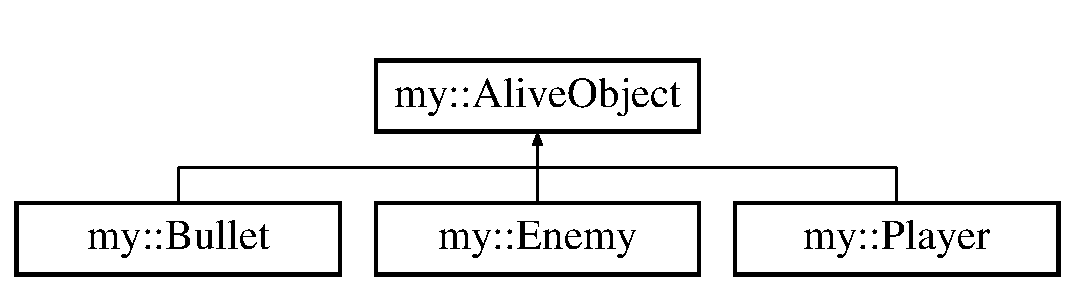
\includegraphics[height=2.000000cm]{classmy_1_1AliveObject}
\end{center}
\end{figure}
\subsection*{Fonctions membres publiques}
\begin{DoxyCompactItemize}
\item 
bool \hyperlink{classmy_1_1AliveObject_ae3d7fb84f66db19cd49e238405590d40}{Is\+Alive} () const noexcept
\begin{DoxyCompactList}\small\item\em Détermine l\textquotesingle{}état de l\textquotesingle{}objet (vivatn ou mort). \end{DoxyCompactList}\item 
unsigned \hyperlink{classmy_1_1AliveObject_ad5c35dbc2ccd74c9edd73fb19b89e6bb}{Get\+Cur\+HP} () const noexcept
\begin{DoxyCompactList}\small\item\em Retourne le nonbre de points de vie courants. \end{DoxyCompactList}\item 
unsigned \hyperlink{classmy_1_1AliveObject_a4537ba5f7d099b5ae2bd59b6db93a76b}{Get\+Max\+HP} () const noexcept
\begin{DoxyCompactList}\small\item\em Retourne le nombre de points de vie maximum. \end{DoxyCompactList}\item 
void \hyperlink{classmy_1_1AliveObject_ae3cf3e26f9fc6b497d8b659621d3ffa8}{Set\+Cur\+HP} (unsigned cur\+HP)  throw (std\+::invalid\+\_\+argument)
\begin{DoxyCompactList}\small\item\em Change le nombre de points de vie courants. \end{DoxyCompactList}\item 
void \hyperlink{classmy_1_1AliveObject_aea104f1424ccb0e2ebca84bd0fba3029}{Set\+Max\+HP} (unsigned max\+HP) noexcept
\begin{DoxyCompactList}\small\item\em Change le nombre de points de vie maximum. \end{DoxyCompactList}\item 
virtual void \hyperlink{classmy_1_1AliveObject_a4c13171af7b862e15bfd1737a75dab75}{Take\+Damage} (unsigned damage) noexcept
\begin{DoxyCompactList}\small\item\em Soustrait aux points de vie courant la valeur passé en argument. \end{DoxyCompactList}\end{DoxyCompactItemize}
\subsection*{Attributs protégés}
\begin{DoxyCompactItemize}
\item 
\mbox{\Hypertarget{classmy_1_1AliveObject_afbeb3d5cebdf6133f3dcace7eea2dff6}\label{classmy_1_1AliveObject_afbeb3d5cebdf6133f3dcace7eea2dff6}} 
bool \hyperlink{classmy_1_1AliveObject_afbeb3d5cebdf6133f3dcace7eea2dff6}{m\+\_\+is\+Alive}
\begin{DoxyCompactList}\small\item\em Booléen déterminant si l\textquotesingle{}objet est \char`\"{}vivant\char`\"{} ou \char`\"{}mort\char`\"{}. \end{DoxyCompactList}\item 
\mbox{\Hypertarget{classmy_1_1AliveObject_a3659debec3ec999e88aa7bdd7ff09fd5}\label{classmy_1_1AliveObject_a3659debec3ec999e88aa7bdd7ff09fd5}} 
unsigned \hyperlink{classmy_1_1AliveObject_a3659debec3ec999e88aa7bdd7ff09fd5}{m\+\_\+\+HP}
\begin{DoxyCompactList}\small\item\em Nombre de points de vie courant. \end{DoxyCompactList}\item 
\mbox{\Hypertarget{classmy_1_1AliveObject_a7c7f74ed8358b08e580462b0d458dd35}\label{classmy_1_1AliveObject_a7c7f74ed8358b08e580462b0d458dd35}} 
unsigned \hyperlink{classmy_1_1AliveObject_a7c7f74ed8358b08e580462b0d458dd35}{m\+\_\+max\+HP}
\begin{DoxyCompactList}\small\item\em Nombre de points de vie maximum. \end{DoxyCompactList}\end{DoxyCompactItemize}
\subsection*{Attributs protégés statiques}
\begin{DoxyCompactItemize}
\item 
\mbox{\Hypertarget{classmy_1_1AliveObject_aa6ebb3bdd0c42782c37f6a42f4744381}\label{classmy_1_1AliveObject_aa6ebb3bdd0c42782c37f6a42f4744381}} 
static const std\+::string \hyperlink{classmy_1_1AliveObject_aa6ebb3bdd0c42782c37f6a42f4744381}{D\+E\+A\+T\+H\+\_\+\+A\+N\+I\+M\+\_\+\+N\+A\+ME} = \char`\"{}death\char`\"{}
\begin{DoxyCompactList}\small\item\em Index de l\textquotesingle{}animation de mort. \end{DoxyCompactList}\end{DoxyCompactItemize}


\subsection{Description détaillée}
Class représentant un object dit \char`\"{}vivant\char`\"{}. 

Un object \char`\"{}vivant\char`\"{} possède un nombre de point de vie maximum et courant, lorsque ces points de vie tombent à 0, l\textquotesingle{}objet est considéré comme \char`\"{}mort\char`\"{} 

\subsection{Documentation des fonctions membres}
\mbox{\Hypertarget{classmy_1_1AliveObject_ad5c35dbc2ccd74c9edd73fb19b89e6bb}\label{classmy_1_1AliveObject_ad5c35dbc2ccd74c9edd73fb19b89e6bb}} 
\index{my\+::\+Alive\+Object@{my\+::\+Alive\+Object}!Get\+Cur\+HP@{Get\+Cur\+HP}}
\index{Get\+Cur\+HP@{Get\+Cur\+HP}!my\+::\+Alive\+Object@{my\+::\+Alive\+Object}}
\subsubsection{\texorpdfstring{Get\+Cur\+H\+P()}{GetCurHP()}}
{\footnotesize\ttfamily unsigned my\+::\+Alive\+Object\+::\+Get\+Cur\+HP (\begin{DoxyParamCaption}{ }\end{DoxyParamCaption}) const\hspace{0.3cm}{\ttfamily [noexcept]}}



Retourne le nonbre de points de vie courants. 

{\bfseries Valeur de retour}~\newline
 Retourne le nombre de points de vie courant dans un entier non-\/signé. \mbox{\Hypertarget{classmy_1_1AliveObject_a4537ba5f7d099b5ae2bd59b6db93a76b}\label{classmy_1_1AliveObject_a4537ba5f7d099b5ae2bd59b6db93a76b}} 
\index{my\+::\+Alive\+Object@{my\+::\+Alive\+Object}!Get\+Max\+HP@{Get\+Max\+HP}}
\index{Get\+Max\+HP@{Get\+Max\+HP}!my\+::\+Alive\+Object@{my\+::\+Alive\+Object}}
\subsubsection{\texorpdfstring{Get\+Max\+H\+P()}{GetMaxHP()}}
{\footnotesize\ttfamily unsigned my\+::\+Alive\+Object\+::\+Get\+Max\+HP (\begin{DoxyParamCaption}{ }\end{DoxyParamCaption}) const\hspace{0.3cm}{\ttfamily [noexcept]}}



Retourne le nombre de points de vie maximum. 

{\bfseries Valeur de retour}~\newline
 Retourne le nombre de points de vie maximum dans un entier non-\/signé. \mbox{\Hypertarget{classmy_1_1AliveObject_ae3d7fb84f66db19cd49e238405590d40}\label{classmy_1_1AliveObject_ae3d7fb84f66db19cd49e238405590d40}} 
\index{my\+::\+Alive\+Object@{my\+::\+Alive\+Object}!Is\+Alive@{Is\+Alive}}
\index{Is\+Alive@{Is\+Alive}!my\+::\+Alive\+Object@{my\+::\+Alive\+Object}}
\subsubsection{\texorpdfstring{Is\+Alive()}{IsAlive()}}
{\footnotesize\ttfamily bool my\+::\+Alive\+Object\+::\+Is\+Alive (\begin{DoxyParamCaption}{ }\end{DoxyParamCaption}) const\hspace{0.3cm}{\ttfamily [noexcept]}}



Détermine l\textquotesingle{}état de l\textquotesingle{}objet (vivatn ou mort). 

{\bfseries Valeur de retour}~\newline
 La fonction retourne {\bfseries vrais} si l\textquotesingle{}objet est vivant, {\bfseries faux} sinon. \mbox{\Hypertarget{classmy_1_1AliveObject_ae3cf3e26f9fc6b497d8b659621d3ffa8}\label{classmy_1_1AliveObject_ae3cf3e26f9fc6b497d8b659621d3ffa8}} 
\index{my\+::\+Alive\+Object@{my\+::\+Alive\+Object}!Set\+Cur\+HP@{Set\+Cur\+HP}}
\index{Set\+Cur\+HP@{Set\+Cur\+HP}!my\+::\+Alive\+Object@{my\+::\+Alive\+Object}}
\subsubsection{\texorpdfstring{Set\+Cur\+H\+P()}{SetCurHP()}}
{\footnotesize\ttfamily void my\+::\+Alive\+Object\+::\+Set\+Cur\+HP (\begin{DoxyParamCaption}\item[{unsigned}]{cur\+HP }\end{DoxyParamCaption}) throw  std\+::invalid\+\_\+argument) }



Change le nombre de points de vie courants. 

{\bfseries Arguments}~\newline
 cur\+HP\+: Le nouveau nombre de points de vie de l\textquotesingle{}objet. ~\newline
~\newline
 {\bfseries Exception}~\newline
 std\+::invalid\+\_\+argument\+: Le nombre de points de vie est supérieur au maximum. \mbox{\Hypertarget{classmy_1_1AliveObject_aea104f1424ccb0e2ebca84bd0fba3029}\label{classmy_1_1AliveObject_aea104f1424ccb0e2ebca84bd0fba3029}} 
\index{my\+::\+Alive\+Object@{my\+::\+Alive\+Object}!Set\+Max\+HP@{Set\+Max\+HP}}
\index{Set\+Max\+HP@{Set\+Max\+HP}!my\+::\+Alive\+Object@{my\+::\+Alive\+Object}}
\subsubsection{\texorpdfstring{Set\+Max\+H\+P()}{SetMaxHP()}}
{\footnotesize\ttfamily void my\+::\+Alive\+Object\+::\+Set\+Max\+HP (\begin{DoxyParamCaption}\item[{unsigned}]{max\+HP }\end{DoxyParamCaption})\hspace{0.3cm}{\ttfamily [noexcept]}}



Change le nombre de points de vie maximum. 

{\bfseries Arguments}~\newline
 max\+HP\+: Le nouveau nombre de points de vie maximum. \mbox{\Hypertarget{classmy_1_1AliveObject_a4c13171af7b862e15bfd1737a75dab75}\label{classmy_1_1AliveObject_a4c13171af7b862e15bfd1737a75dab75}} 
\index{my\+::\+Alive\+Object@{my\+::\+Alive\+Object}!Take\+Damage@{Take\+Damage}}
\index{Take\+Damage@{Take\+Damage}!my\+::\+Alive\+Object@{my\+::\+Alive\+Object}}
\subsubsection{\texorpdfstring{Take\+Damage()}{TakeDamage()}}
{\footnotesize\ttfamily void my\+::\+Alive\+Object\+::\+Take\+Damage (\begin{DoxyParamCaption}\item[{unsigned}]{damage }\end{DoxyParamCaption})\hspace{0.3cm}{\ttfamily [virtual]}, {\ttfamily [noexcept]}}



Soustrait aux points de vie courant la valeur passé en argument. 

{\bfseries Arguments}~\newline
 damage\+: Le nombre de dommage à subir. 

Réimplémentée dans \hyperlink{classmy_1_1Bullet_add56b393dfba4c70de2713d4a3c917c3}{my\+::\+Bullet}, et \hyperlink{classmy_1_1Enemy_a38251585de243212ad04d5bbc2843f50}{my\+::\+Enemy}.



La documentation de cette classe a été générée à partir des fichiers suivants \+:\begin{DoxyCompactItemize}
\item 
includes/my\+\_\+objects\+\_\+lib/Alive\+Object.\+hpp\item 
lib/my\+\_\+objects\+\_\+lib/Alive\+Object.\+cpp\end{DoxyCompactItemize}

\hypertarget{classmy_1_1AnimatedObject}{}\section{Référence de la classe my\+:\+:Animated\+Object}
\label{classmy_1_1AnimatedObject}\index{my\+::\+Animated\+Object@{my\+::\+Animated\+Object}}
Graphe d\textquotesingle{}héritage de my\+:\+:Animated\+Object\+:\begin{figure}[H]
\begin{center}
\leavevmode
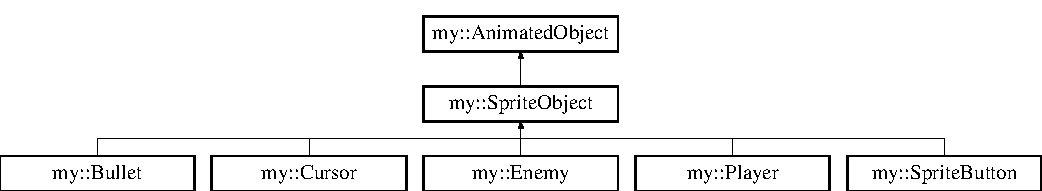
\includegraphics[height=2.564885cm]{classmy_1_1AnimatedObject}
\end{center}
\end{figure}
\subsection*{Classes}
\begin{DoxyCompactItemize}
\item 
struct \hyperlink{structmy_1_1AnimatedObject_1_1Animation}{Animation}
\end{DoxyCompactItemize}
\subsection*{Types publics}
\begin{DoxyCompactItemize}
\item 
\mbox{\Hypertarget{classmy_1_1AnimatedObject_a15ca4fc03c83bb613ce972f422ab5ccd}\label{classmy_1_1AnimatedObject_a15ca4fc03c83bb613ce972f422ab5ccd}} 
typedef std\+::shared\+\_\+ptr$<$ \hyperlink{classmy_1_1AnimatedObject}{Animated\+Object} $>$ {\bfseries Animated\+Object\+Ptr}
\item 
\mbox{\Hypertarget{classmy_1_1AnimatedObject_aae6a82042023277647171b52de887b85}\label{classmy_1_1AnimatedObject_aae6a82042023277647171b52de887b85}} 
typedef std\+::vector$<$ \hyperlink{structmy_1_1AnimatedObject_1_1Animation}{Animation} $>$ {\bfseries Animations}
\end{DoxyCompactItemize}
\subsection*{Fonctions membres publiques}
\begin{DoxyCompactItemize}
\item 
\mbox{\Hypertarget{classmy_1_1AnimatedObject_a480119012567dd5f2012b61eaf6c8273}\label{classmy_1_1AnimatedObject_a480119012567dd5f2012b61eaf6c8273}} 
bool {\bfseries Is\+On\+Animation} () const noexcept
\item 
\mbox{\Hypertarget{classmy_1_1AnimatedObject_a49756a252ea70f3113619f1666205794}\label{classmy_1_1AnimatedObject_a49756a252ea70f3113619f1666205794}} 
bool {\bfseries Animation\+Exist} (const std\+::string \&key) const noexcept
\item 
\mbox{\Hypertarget{classmy_1_1AnimatedObject_a6aabe49b2c026eeb609c1a558141e241}\label{classmy_1_1AnimatedObject_a6aabe49b2c026eeb609c1a558141e241}} 
const sf\+::\+Int\+Rect \& {\bfseries Get\+Curent\+Rect} () const  throw (std\+::out\+\_\+of\+\_\+range)
\item 
\mbox{\Hypertarget{classmy_1_1AnimatedObject_ab5a32b5d7b30e6ca594d824a8228b0df}\label{classmy_1_1AnimatedObject_ab5a32b5d7b30e6ca594d824a8228b0df}} 
const \hyperlink{structmy_1_1AnimatedObject_1_1Animation}{Animation} \& {\bfseries Get\+Curent\+Animation} () const  throw (std\+::out\+\_\+of\+\_\+range)
\item 
\mbox{\Hypertarget{classmy_1_1AnimatedObject_a41aafdead3b867bd67ce633fb85ed9af}\label{classmy_1_1AnimatedObject_a41aafdead3b867bd67ce633fb85ed9af}} 
const Animations \& {\bfseries Get\+Animations} () const noexcept
\item 
\mbox{\Hypertarget{classmy_1_1AnimatedObject_aa786264957518722eb2b847fa725e3b1}\label{classmy_1_1AnimatedObject_aa786264957518722eb2b847fa725e3b1}} 
unsigned {\bfseries Get\+Cur\+Framerate} () const noexcept
\item 
\mbox{\Hypertarget{classmy_1_1AnimatedObject_a0e01eea3aec59eace02d377bcf3f528d}\label{classmy_1_1AnimatedObject_a0e01eea3aec59eace02d377bcf3f528d}} 
void {\bfseries Set\+On\+Animation} (bool on\+Animation) noexcept
\item 
\mbox{\Hypertarget{classmy_1_1AnimatedObject_a528df17be1a66e7ead821c3a0de3609b}\label{classmy_1_1AnimatedObject_a528df17be1a66e7ead821c3a0de3609b}} 
void {\bfseries Set\+Animations} (const Animations \&animations) noexcept
\item 
\mbox{\Hypertarget{classmy_1_1AnimatedObject_aa280439191dcecdb95ca210a5d0901da}\label{classmy_1_1AnimatedObject_aa280439191dcecdb95ca210a5d0901da}} 
void {\bfseries Add\+Animation} (const \hyperlink{structmy_1_1AnimatedObject_1_1Animation}{Animation} \&animation) noexcept
\item 
\mbox{\Hypertarget{classmy_1_1AnimatedObject_a4efb6bb97d338e7008c84800ab7c3802}\label{classmy_1_1AnimatedObject_a4efb6bb97d338e7008c84800ab7c3802}} 
void {\bfseries Set\+Anim\+Index} (int index, int tile\+Index=0)  throw (std\+::out\+\_\+of\+\_\+range)
\item 
\mbox{\Hypertarget{classmy_1_1AnimatedObject_ab48589255e1825b37c68b25522de2b94}\label{classmy_1_1AnimatedObject_ab48589255e1825b37c68b25522de2b94}} 
void {\bfseries Set\+Anim\+Index} (const std\+::string \&key, int tile\+Index=0)  throw (std\+::out\+\_\+of\+\_\+range)
\item 
\mbox{\Hypertarget{classmy_1_1AnimatedObject_aa4e740cdea42f3531264a3b438d7482d}\label{classmy_1_1AnimatedObject_aa4e740cdea42f3531264a3b438d7482d}} 
void {\bfseries Set\+Anim\+Tile\+Index} (int tile\+Index)  throw (std\+::out\+\_\+of\+\_\+range)
\item 
\mbox{\Hypertarget{classmy_1_1AnimatedObject_a6c79b593a1fec85a831ec94a38f94c83}\label{classmy_1_1AnimatedObject_a6c79b593a1fec85a831ec94a38f94c83}} 
void {\bfseries Set\+Cur\+Frame\+Rate} (unsigned cur\+Framerate) noexcept
\end{DoxyCompactItemize}
\subsection*{Fonctions membres protégées}
\begin{DoxyCompactItemize}
\item 
\mbox{\Hypertarget{classmy_1_1AnimatedObject_a3191de9eb8f6cff2f5392638fa13cca3}\label{classmy_1_1AnimatedObject_a3191de9eb8f6cff2f5392638fa13cca3}} 
virtual void {\bfseries Update\+Animation} ()  throw (std\+::out\+\_\+of\+\_\+range)
\end{DoxyCompactItemize}
\subsection*{Attributs protégés}
\begin{DoxyCompactItemize}
\item 
\mbox{\Hypertarget{classmy_1_1AnimatedObject_adc14c5e8effd46c532ca02127ba1a189}\label{classmy_1_1AnimatedObject_adc14c5e8effd46c532ca02127ba1a189}} 
bool {\bfseries m\+\_\+on\+Animation}
\item 
\mbox{\Hypertarget{classmy_1_1AnimatedObject_a553266e96f728842249f960687d094b9}\label{classmy_1_1AnimatedObject_a553266e96f728842249f960687d094b9}} 
Animations {\bfseries m\+\_\+animations}
\item 
\mbox{\Hypertarget{classmy_1_1AnimatedObject_a0a660f4d34009beb751bb8d8d16652af}\label{classmy_1_1AnimatedObject_a0a660f4d34009beb751bb8d8d16652af}} 
int {\bfseries m\+\_\+anim\+Index}
\item 
\mbox{\Hypertarget{classmy_1_1AnimatedObject_a1b115d7e8e1919079b669c87466f56a2}\label{classmy_1_1AnimatedObject_a1b115d7e8e1919079b669c87466f56a2}} 
int {\bfseries m\+\_\+anim\+Tile\+Index}
\item 
\mbox{\Hypertarget{classmy_1_1AnimatedObject_a49fddef498a3975e4846cf093e83e41f}\label{classmy_1_1AnimatedObject_a49fddef498a3975e4846cf093e83e41f}} 
unsigned {\bfseries m\+\_\+cur\+Framerate}
\end{DoxyCompactItemize}
\subsection*{Attributs protégés statiques}
\begin{DoxyCompactItemize}
\item 
\mbox{\Hypertarget{classmy_1_1AnimatedObject_a561669375b8ea9b5be6309c04be3056b}\label{classmy_1_1AnimatedObject_a561669375b8ea9b5be6309c04be3056b}} 
static const std\+::string {\bfseries D\+E\+F\+A\+U\+L\+T\+\_\+\+A\+N\+I\+M\+\_\+\+N\+A\+ME} = \char`\"{}default\char`\"{}
\end{DoxyCompactItemize}


La documentation de cette classe a été générée à partir des fichiers suivants \+:\begin{DoxyCompactItemize}
\item 
includes/my\+\_\+graph\+\_\+lib/Animated\+Object.\+hpp\item 
lib/my\+\_\+graph\+\_\+lib/Animated\+Object.\+cpp\end{DoxyCompactItemize}

\hypertarget{structmy_1_1AnimatedObject_1_1Animation}{}\section{Référence de la structure my\+:\+:Animated\+Object\+:\+:Animation}
\label{structmy_1_1AnimatedObject_1_1Animation}\index{my\+::\+Animated\+Object\+::\+Animation@{my\+::\+Animated\+Object\+::\+Animation}}
\subsection*{Types publics}
\begin{DoxyCompactItemize}
\item 
\mbox{\Hypertarget{structmy_1_1AnimatedObject_1_1Animation_af3f7283fa1832cc314b21aecc3ae7367}\label{structmy_1_1AnimatedObject_1_1Animation_af3f7283fa1832cc314b21aecc3ae7367}} 
typedef std\+::vector$<$ sf\+::\+Int\+Rect $>$ {\bfseries Animation\+Rects}
\end{DoxyCompactItemize}
\subsection*{Attributs publics}
\begin{DoxyCompactItemize}
\item 
\mbox{\Hypertarget{structmy_1_1AnimatedObject_1_1Animation_a303859b9ae4ab314a9b90b90dca55139}\label{structmy_1_1AnimatedObject_1_1Animation_a303859b9ae4ab314a9b90b90dca55139}} 
Animation\+Rects {\bfseries rects}
\item 
\mbox{\Hypertarget{structmy_1_1AnimatedObject_1_1Animation_ae486a77dd2ca108c52d1620f2723491d}\label{structmy_1_1AnimatedObject_1_1Animation_ae486a77dd2ca108c52d1620f2723491d}} 
unsigned {\bfseries framerate\+Max}
\item 
\mbox{\Hypertarget{structmy_1_1AnimatedObject_1_1Animation_a109781da110faff4ee36450a945153ba}\label{structmy_1_1AnimatedObject_1_1Animation_a109781da110faff4ee36450a945153ba}} 
std\+::string {\bfseries key}
\item 
\mbox{\Hypertarget{structmy_1_1AnimatedObject_1_1Animation_a37d8637ca7e02b062a48b35795f23d85}\label{structmy_1_1AnimatedObject_1_1Animation_a37d8637ca7e02b062a48b35795f23d85}} 
bool {\bfseries loop}
\end{DoxyCompactItemize}


La documentation de cette structure a été générée à partir du fichier suivant \+:\begin{DoxyCompactItemize}
\item 
includes/my\+\_\+graph\+\_\+lib/Animated\+Object.\+hpp\end{DoxyCompactItemize}

\hypertarget{classmy_1_1Border}{}\section{Référence de la classe my\+:\+:Border}
\label{classmy_1_1Border}\index{my\+::\+Border@{my\+::\+Border}}
Graphe d\textquotesingle{}héritage de my\+:\+:Border\+:\begin{figure}[H]
\begin{center}
\leavevmode
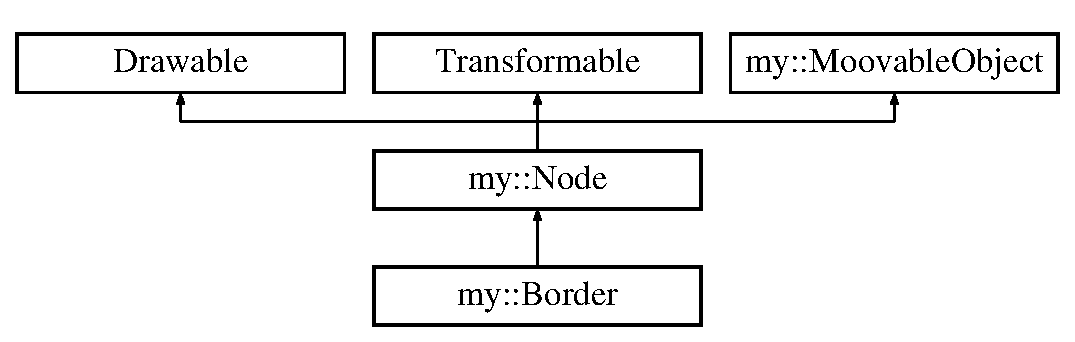
\includegraphics[height=3.000000cm]{classmy_1_1Border}
\end{center}
\end{figure}
\subsection*{Types publics}
\begin{DoxyCompactItemize}
\item 
\mbox{\Hypertarget{classmy_1_1Border_ac25a32ed037962d5513c63e60a510f8e}\label{classmy_1_1Border_ac25a32ed037962d5513c63e60a510f8e}} 
typedef std\+::shared\+\_\+ptr$<$ \hyperlink{classmy_1_1Border}{Border} $>$ {\bfseries Border\+Ptr}
\item 
\mbox{\Hypertarget{classmy_1_1Border_a183b7d4c2bd05d33120eccd7b1c38680}\label{classmy_1_1Border_a183b7d4c2bd05d33120eccd7b1c38680}} 
typedef Sprite\+Object\+::\+Sprite\+Object\+Ptr {\bfseries Tile}
\item 
\mbox{\Hypertarget{classmy_1_1Border_a71eaaf9ddced3cb6ca06df43d460cf80}\label{classmy_1_1Border_a71eaaf9ddced3cb6ca06df43d460cf80}} 
typedef std\+::vector$<$ Tile $>$ {\bfseries Tile\+List}
\end{DoxyCompactItemize}
\subsection*{Fonctions membres publiques}
\begin{DoxyCompactItemize}
\item 
\mbox{\Hypertarget{classmy_1_1Border_acf58f88a4e6085ddd0f2c63dd5ea0ff5}\label{classmy_1_1Border_acf58f88a4e6085ddd0f2c63dd5ea0ff5}} 
bool {\bfseries Is\+Intersect} (const sf\+::\+Vector2f \&point) const noexcept
\item 
\mbox{\Hypertarget{classmy_1_1Border_aa65c4ff4d89fef5edea53a594b32a8cc}\label{classmy_1_1Border_aa65c4ff4d89fef5edea53a594b32a8cc}} 
bool {\bfseries Is\+Intersect} (const sf\+::\+Float\+Rect \&square) const noexcept
\item 
\mbox{\Hypertarget{classmy_1_1Border_aab075f5fda8f39ce5cb1fc7fc42cd0b4}\label{classmy_1_1Border_aab075f5fda8f39ce5cb1fc7fc42cd0b4}} 
const sf\+::\+Float\+Rect {\bfseries Get\+Hit\+Box} () const noexcept
\item 
\mbox{\Hypertarget{classmy_1_1Border_ab897d683eb3f4e4484f0a23ed419a9e7}\label{classmy_1_1Border_ab897d683eb3f4e4484f0a23ed419a9e7}} 
const std\+::string \& {\bfseries Get\+Texture\+Key} () const noexcept
\item 
\mbox{\Hypertarget{classmy_1_1Border_a7235f7cff623e59370b6a044b4cbb060}\label{classmy_1_1Border_a7235f7cff623e59370b6a044b4cbb060}} 
const sf\+::\+Vector2u \& {\bfseries Get\+Size} () const noexcept
\item 
\mbox{\Hypertarget{classmy_1_1Border_aaaf6ddc65bc19ffb54f352df35c94090}\label{classmy_1_1Border_aaaf6ddc65bc19ffb54f352df35c94090}} 
const sf\+::\+Vector2u \& {\bfseries Get\+Tile\+Size} () const noexcept
\item 
\mbox{\Hypertarget{classmy_1_1Border_a8da811b24ad62ebb53a9363567f607c7}\label{classmy_1_1Border_a8da811b24ad62ebb53a9363567f607c7}} 
const sf\+::\+Int\+Rect \& {\bfseries Get\+Corner\+Subrect} () const noexcept
\item 
\mbox{\Hypertarget{classmy_1_1Border_ad8f5806d2521b3b5c1d7c03bd4b18958}\label{classmy_1_1Border_ad8f5806d2521b3b5c1d7c03bd4b18958}} 
const sf\+::\+Int\+Rect \& {\bfseries Get\+Outline\+Subrect} () const noexcept
\item 
\mbox{\Hypertarget{classmy_1_1Border_a1d9d83ce552ad3a2fb90cfc496b5e885}\label{classmy_1_1Border_a1d9d83ce552ad3a2fb90cfc496b5e885}} 
const Tile\+List \& {\bfseries Get\+Tiles} () const noexcept
\item 
\mbox{\Hypertarget{classmy_1_1Border_aa162c706bd04538df15c358618ec56e2}\label{classmy_1_1Border_aa162c706bd04538df15c358618ec56e2}} 
void {\bfseries Set\+Texture\+Key} (const std\+::string \&texture\+Key) noexcept
\item 
\mbox{\Hypertarget{classmy_1_1Border_adc7560e9269a9de9f7f2a88b154e520d}\label{classmy_1_1Border_adc7560e9269a9de9f7f2a88b154e520d}} 
void {\bfseries Set\+Size} (const sf\+::\+Vector2u \&size) noexcept
\item 
\mbox{\Hypertarget{classmy_1_1Border_a9b095f0dafa161744f6f8a113d4bc021}\label{classmy_1_1Border_a9b095f0dafa161744f6f8a113d4bc021}} 
void {\bfseries Set\+Tile\+Size} (const sf\+::\+Vector2u \&tile\+Size) noexcept
\item 
\mbox{\Hypertarget{classmy_1_1Border_a8bd8d973b026bc4568e01d5345b4f2b3}\label{classmy_1_1Border_a8bd8d973b026bc4568e01d5345b4f2b3}} 
void {\bfseries Set\+Corner\+Subrect} (const sf\+::\+Int\+Rect \&corner\+Subrect) noexcept
\item 
\mbox{\Hypertarget{classmy_1_1Border_a34fffa6602d617e7e5907a8a52f60583}\label{classmy_1_1Border_a34fffa6602d617e7e5907a8a52f60583}} 
void {\bfseries Set\+Outline\+Subrect} (const sf\+::\+Int\+Rect \&outline\+Subrect) noexcept
\item 
\mbox{\Hypertarget{classmy_1_1Border_a18a8fac0b1abec5a98b74f9ec9d38464}\label{classmy_1_1Border_a18a8fac0b1abec5a98b74f9ec9d38464}} 
void {\bfseries Initialize\+Childs} ()  throw (std\+::invalid\+\_\+argument)
\item 
\mbox{\Hypertarget{classmy_1_1Border_a02315dc4d26d3e31b68bb05c9759aa57}\label{classmy_1_1Border_a02315dc4d26d3e31b68bb05c9759aa57}} 
void {\bfseries Update\+Tiles} () noexcept
\end{DoxyCompactItemize}
\subsection*{Membres hérités additionnels}


La documentation de cette classe a été générée à partir des fichiers suivants \+:\begin{DoxyCompactItemize}
\item 
includes/my\+\_\+objects\+\_\+lib/Border.\+hpp\item 
lib/my\+\_\+objects\+\_\+lib/Border.\+cpp\end{DoxyCompactItemize}

\hypertarget{classmy_1_1Bullet}{}\section{Référence de la classe my\+:\+:Bullet}
\label{classmy_1_1Bullet}\index{my\+::\+Bullet@{my\+::\+Bullet}}
Graphe d\textquotesingle{}héritage de my\+:\+:Bullet\+:\begin{figure}[H]
\begin{center}
\leavevmode
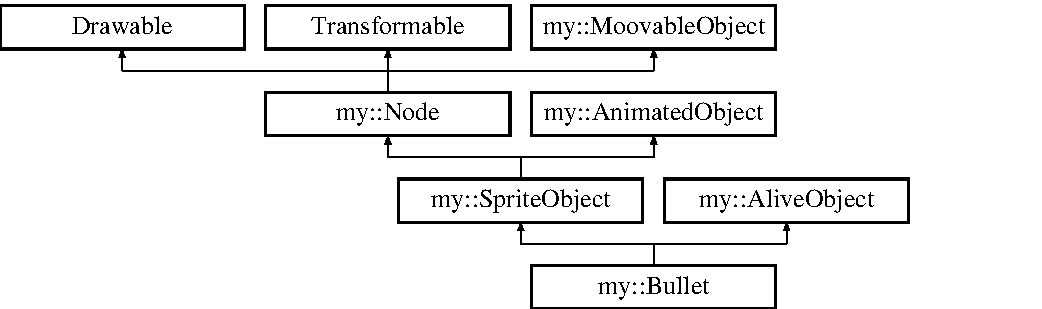
\includegraphics[height=4.000000cm]{classmy_1_1Bullet}
\end{center}
\end{figure}
\subsection*{Types publics}
\begin{DoxyCompactItemize}
\item 
\mbox{\Hypertarget{classmy_1_1Bullet_a4b5c005e88ac1169b45ef54969763ddf}\label{classmy_1_1Bullet_a4b5c005e88ac1169b45ef54969763ddf}} 
typedef std\+::shared\+\_\+ptr$<$ \hyperlink{classmy_1_1Bullet}{Bullet} $>$ {\bfseries Bullet\+Ptr}
\end{DoxyCompactItemize}
\subsection*{Fonctions membres publiques}
\begin{DoxyCompactItemize}
\item 
\mbox{\Hypertarget{classmy_1_1Bullet_a4d8f83b7d45b3a427ef622b30504c994}\label{classmy_1_1Bullet_a4d8f83b7d45b3a427ef622b30504c994}} 
virtual void {\bfseries Update} ()  throw (std\+::out\+\_\+of\+\_\+range)
\item 
virtual void \hyperlink{classmy_1_1Bullet_add56b393dfba4c70de2713d4a3c917c3}{Take\+Damage} (unsigned damage) noexcept
\begin{DoxyCompactList}\small\item\em Soustrait aux points de vie courant la valeur passé en argument. \end{DoxyCompactList}\item 
\mbox{\Hypertarget{classmy_1_1Bullet_ac09bef4306b861082d6faf51ffa196ec}\label{classmy_1_1Bullet_ac09bef4306b861082d6faf51ffa196ec}} 
bool {\bfseries Is\+Finish} () const noexcept
\item 
\mbox{\Hypertarget{classmy_1_1Bullet_ae27237c0484100a583acb3c1368ac748}\label{classmy_1_1Bullet_ae27237c0484100a583acb3c1368ac748}} 
unsigned {\bfseries Get\+Travel\+Time} () const noexcept
\item 
\mbox{\Hypertarget{classmy_1_1Bullet_aa892fbd61eb8400b1edc0510f520222f}\label{classmy_1_1Bullet_aa892fbd61eb8400b1edc0510f520222f}} 
unsigned {\bfseries Get\+Damage} () const noexcept
\item 
\mbox{\Hypertarget{classmy_1_1Bullet_abce688ee87e4fc3127138ffa9188a176}\label{classmy_1_1Bullet_abce688ee87e4fc3127138ffa9188a176}} 
void {\bfseries Set\+Travel\+Time} (unsigned travel\+Time) noexcept
\item 
\mbox{\Hypertarget{classmy_1_1Bullet_ae283ab2faf88aa846a59df9eb52b5c10}\label{classmy_1_1Bullet_ae283ab2faf88aa846a59df9eb52b5c10}} 
void {\bfseries Set\+Damage} (unsigned damage) noexcept
\end{DoxyCompactItemize}
\subsection*{Fonctions membres protégées}
\begin{DoxyCompactItemize}
\item 
\mbox{\Hypertarget{classmy_1_1Bullet_a6cf422fe6c782a0455a21fa38b999464}\label{classmy_1_1Bullet_a6cf422fe6c782a0455a21fa38b999464}} 
virtual void {\bfseries Update\+Animation} ()  throw (std\+::out\+\_\+of\+\_\+range)
\end{DoxyCompactItemize}
\subsection*{Attributs protégés}
\begin{DoxyCompactItemize}
\item 
\mbox{\Hypertarget{classmy_1_1Bullet_ae24f81c42c087ec24378674c27f749a0}\label{classmy_1_1Bullet_ae24f81c42c087ec24378674c27f749a0}} 
unsigned {\bfseries m\+\_\+travel\+Time}
\item 
\mbox{\Hypertarget{classmy_1_1Bullet_ab06dc2584a017781b2cf592d906c14da}\label{classmy_1_1Bullet_ab06dc2584a017781b2cf592d906c14da}} 
unsigned {\bfseries m\+\_\+damage}
\end{DoxyCompactItemize}
\subsection*{Membres hérités additionnels}


\subsection{Documentation des fonctions membres}
\mbox{\Hypertarget{classmy_1_1Bullet_add56b393dfba4c70de2713d4a3c917c3}\label{classmy_1_1Bullet_add56b393dfba4c70de2713d4a3c917c3}} 
\index{my\+::\+Bullet@{my\+::\+Bullet}!Take\+Damage@{Take\+Damage}}
\index{Take\+Damage@{Take\+Damage}!my\+::\+Bullet@{my\+::\+Bullet}}
\subsubsection{\texorpdfstring{Take\+Damage()}{TakeDamage()}}
{\footnotesize\ttfamily void my\+::\+Bullet\+::\+Take\+Damage (\begin{DoxyParamCaption}\item[{unsigned}]{damage }\end{DoxyParamCaption})\hspace{0.3cm}{\ttfamily [virtual]}, {\ttfamily [noexcept]}}



Soustrait aux points de vie courant la valeur passé en argument. 

{\bfseries Arguments}~\newline
 damage\+: Le nombre de dommage à subir. 

Réimplémentée à partir de \hyperlink{classmy_1_1AliveObject_a4c13171af7b862e15bfd1737a75dab75}{my\+::\+Alive\+Object}.



La documentation de cette classe a été générée à partir des fichiers suivants \+:\begin{DoxyCompactItemize}
\item 
includes/my\+\_\+objects\+\_\+lib/Bullet.\+hpp\item 
lib/my\+\_\+objects\+\_\+lib/Bullet.\+cpp\end{DoxyCompactItemize}

\hypertarget{classmy_1_1Cursor}{}\section{Référence de la classe my\+:\+:Cursor}
\label{classmy_1_1Cursor}\index{my\+::\+Cursor@{my\+::\+Cursor}}
Graphe d\textquotesingle{}héritage de my\+:\+:Cursor\+:\begin{figure}[H]
\begin{center}
\leavevmode
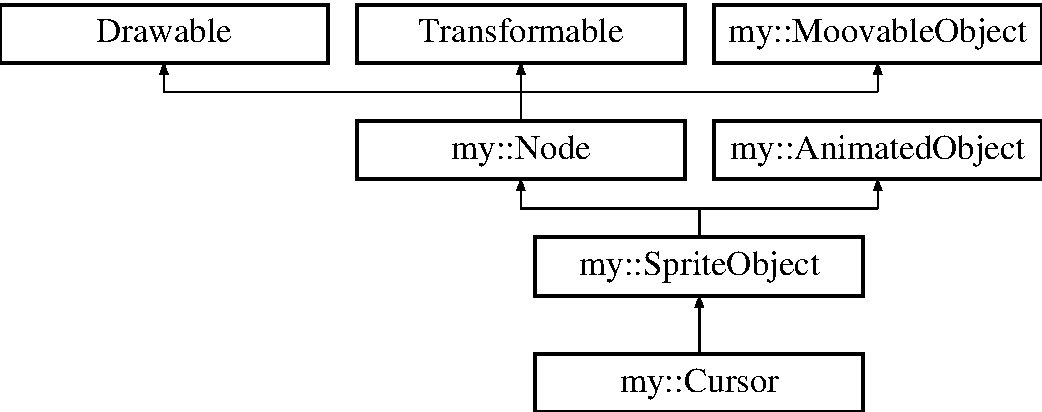
\includegraphics[height=4.000000cm]{classmy_1_1Cursor}
\end{center}
\end{figure}
\subsection*{Types publics}
\begin{DoxyCompactItemize}
\item 
\mbox{\Hypertarget{classmy_1_1Cursor_afbf71f356d765e088f505464bcfac84a}\label{classmy_1_1Cursor_afbf71f356d765e088f505464bcfac84a}} 
typedef std\+::shared\+\_\+ptr$<$ \hyperlink{classmy_1_1Cursor}{Cursor} $>$ {\bfseries Cursor\+Ptr}
\end{DoxyCompactItemize}
\subsection*{Fonctions membres publiques}
\begin{DoxyCompactItemize}
\item 
\mbox{\Hypertarget{classmy_1_1Cursor_abe2aa1caac7aca369c8d8383458323d1}\label{classmy_1_1Cursor_abe2aa1caac7aca369c8d8383458323d1}} 
void {\bfseries Update} (const sf\+::\+Vector2f \&mouse\+Pos)  throw (std\+::out\+\_\+of\+\_\+range)
\end{DoxyCompactItemize}
\subsection*{Membres hérités additionnels}


La documentation de cette classe a été générée à partir des fichiers suivants \+:\begin{DoxyCompactItemize}
\item 
includes/my\+\_\+objects\+\_\+lib/Cursor.\+hpp\item 
lib/my\+\_\+objects\+\_\+lib/Cursor.\+cpp\end{DoxyCompactItemize}

\hypertarget{classmy_1_1EnemiesPool}{}\section{Référence de la classe my\+:\+:Enemies\+Pool}
\label{classmy_1_1EnemiesPool}\index{my\+::\+Enemies\+Pool@{my\+::\+Enemies\+Pool}}
\subsection*{Types publics}
\begin{DoxyCompactItemize}
\item 
\mbox{\Hypertarget{classmy_1_1EnemiesPool_ae3f32bbf808d2bf78926b3d9833baa0b}\label{classmy_1_1EnemiesPool_ae3f32bbf808d2bf78926b3d9833baa0b}} 
typedef std\+::vector$<$ Enemy\+::\+Enemy\+Ptr $>$ {\bfseries Enemies\+List}
\item 
\mbox{\Hypertarget{classmy_1_1EnemiesPool_a802897ecaf9a2be0342fe0c940d8b87d}\label{classmy_1_1EnemiesPool_a802897ecaf9a2be0342fe0c940d8b87d}} 
typedef std\+::vector$<$ X\+M\+L\+Node\+::\+X\+M\+L\+Node\+Ptr $>$ {\bfseries Enemies\+Node\+List}
\end{DoxyCompactItemize}
\subsection*{Fonctions membres publiques}
\begin{DoxyCompactItemize}
\item 
\mbox{\Hypertarget{classmy_1_1EnemiesPool_ac19b1fb3fa34c79ecd8a113f56838ef2}\label{classmy_1_1EnemiesPool_ac19b1fb3fa34c79ecd8a113f56838ef2}} 
void {\bfseries Initialize\+Stage} (X\+M\+L\+Node\+::\+X\+M\+L\+Node\+Ptr stage\+Node)  throw (std\+::out\+\_\+of\+\_\+range, std\+::invalid\+\_\+argument)
\item 
\mbox{\Hypertarget{classmy_1_1EnemiesPool_a8014f3ffa9485b428ed2cc5b8cc656a6}\label{classmy_1_1EnemiesPool_a8014f3ffa9485b428ed2cc5b8cc656a6}} 
void {\bfseries Initialize\+Enemies} (X\+M\+L\+Node\+::\+X\+M\+L\+Node\+Ptr enemies\+Node)  throw (std\+::out\+\_\+of\+\_\+range, std\+::invalid\+\_\+argument)
\item 
\mbox{\Hypertarget{classmy_1_1EnemiesPool_afb428383f257a2e10cc1e6b4cea42a26}\label{classmy_1_1EnemiesPool_afb428383f257a2e10cc1e6b4cea42a26}} 
const Enemies\+List {\bfseries Update} (bool is\+Clean)  throw (std\+::out\+\_\+of\+\_\+range, std\+::invalid\+\_\+argument)
\end{DoxyCompactItemize}


La documentation de cette classe a été générée à partir des fichiers suivants \+:\begin{DoxyCompactItemize}
\item 
includes/my\+\_\+objects\+\_\+lib/Enemies\+Pool.\+hpp\item 
lib/my\+\_\+objects\+\_\+lib/Enemies\+Pool.\+cpp\end{DoxyCompactItemize}

\hypertarget{classmy_1_1Enemy}{}\section{Référence de la classe my\+:\+:Enemy}
\label{classmy_1_1Enemy}\index{my\+::\+Enemy@{my\+::\+Enemy}}
Graphe d\textquotesingle{}héritage de my\+:\+:Enemy\+:\begin{figure}[H]
\begin{center}
\leavevmode
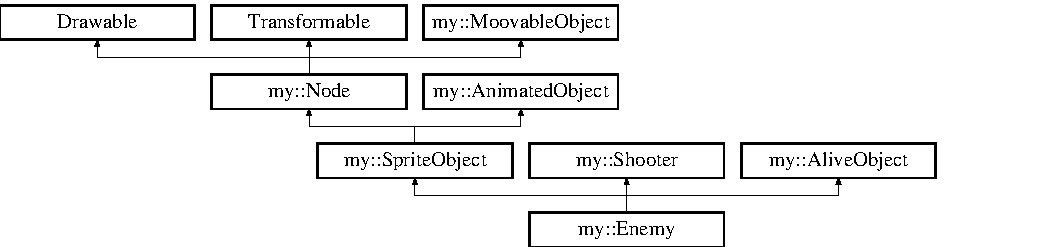
\includegraphics[height=3.318518cm]{classmy_1_1Enemy}
\end{center}
\end{figure}
\subsection*{Types publics}
\begin{DoxyCompactItemize}
\item 
\mbox{\Hypertarget{classmy_1_1Enemy_a641a329df8e8ebbe703e7dfe81968ba3}\label{classmy_1_1Enemy_a641a329df8e8ebbe703e7dfe81968ba3}} 
typedef std\+::shared\+\_\+ptr$<$ \hyperlink{classmy_1_1Enemy}{Enemy} $>$ {\bfseries Enemy\+Ptr}
\end{DoxyCompactItemize}
\subsection*{Fonctions membres publiques}
\begin{DoxyCompactItemize}
\item 
\mbox{\Hypertarget{classmy_1_1Enemy_ae6f0f34e1aedd39a7b6b1d59dc15d9ec}\label{classmy_1_1Enemy_ae6f0f34e1aedd39a7b6b1d59dc15d9ec}} 
virtual void {\bfseries Update} ()  throw (std\+::out\+\_\+of\+\_\+range)
\item 
virtual void \hyperlink{classmy_1_1Enemy_a38251585de243212ad04d5bbc2843f50}{Take\+Damage} (unsigned damage) noexcept
\begin{DoxyCompactList}\small\item\em Soustrait aux points de vie courant la valeur passé en argument. \end{DoxyCompactList}\item 
\mbox{\Hypertarget{classmy_1_1Enemy_a0cc3f61e52ef9de7902d81e6be6be3ff}\label{classmy_1_1Enemy_a0cc3f61e52ef9de7902d81e6be6be3ff}} 
bool {\bfseries Is\+Finish} () const noexcept
\item 
\mbox{\Hypertarget{classmy_1_1Enemy_a627abffea3eda8d0e849523452faf20b}\label{classmy_1_1Enemy_a627abffea3eda8d0e849523452faf20b}} 
void {\bfseries Set\+Is\+Finish} (bool is\+Finish) noexcept
\end{DoxyCompactItemize}
\subsection*{Fonctions membres protégées}
\begin{DoxyCompactItemize}
\item 
\mbox{\Hypertarget{classmy_1_1Enemy_a2257e77a7afcea3a210ffb0ea8f2806e}\label{classmy_1_1Enemy_a2257e77a7afcea3a210ffb0ea8f2806e}} 
virtual void {\bfseries Update\+Animation} ()  throw (std\+::out\+\_\+of\+\_\+range)
\end{DoxyCompactItemize}
\subsection*{Attributs protégés}
\begin{DoxyCompactItemize}
\item 
\mbox{\Hypertarget{classmy_1_1Enemy_ae931fb8aca0540eeaf99e28cb2098793}\label{classmy_1_1Enemy_ae931fb8aca0540eeaf99e28cb2098793}} 
bool {\bfseries m\+\_\+is\+Finish}
\end{DoxyCompactItemize}
\subsection*{Membres hérités additionnels}


\subsection{Documentation des fonctions membres}
\mbox{\Hypertarget{classmy_1_1Enemy_a38251585de243212ad04d5bbc2843f50}\label{classmy_1_1Enemy_a38251585de243212ad04d5bbc2843f50}} 
\index{my\+::\+Enemy@{my\+::\+Enemy}!Take\+Damage@{Take\+Damage}}
\index{Take\+Damage@{Take\+Damage}!my\+::\+Enemy@{my\+::\+Enemy}}
\subsubsection{\texorpdfstring{Take\+Damage()}{TakeDamage()}}
{\footnotesize\ttfamily void my\+::\+Enemy\+::\+Take\+Damage (\begin{DoxyParamCaption}\item[{unsigned}]{damage }\end{DoxyParamCaption})\hspace{0.3cm}{\ttfamily [virtual]}, {\ttfamily [noexcept]}}



Soustrait aux points de vie courant la valeur passé en argument. 

{\bfseries Arguments}~\newline
 damage\+: Le nombre de dommage à subir. 

Réimplémentée à partir de \hyperlink{classmy_1_1AliveObject_a4c13171af7b862e15bfd1737a75dab75}{my\+::\+Alive\+Object}.



La documentation de cette classe a été générée à partir des fichiers suivants \+:\begin{DoxyCompactItemize}
\item 
includes/my\+\_\+objects\+\_\+lib/Enemy.\+hpp\item 
lib/my\+\_\+objects\+\_\+lib/Enemy.\+cpp\end{DoxyCompactItemize}

\hypertarget{classmy_1_1GameManager}{}\section{Référence de la classe my\+:\+:Game\+Manager}
\label{classmy_1_1GameManager}\index{my\+::\+Game\+Manager@{my\+::\+Game\+Manager}}


Class principal du jeux.  




{\ttfamily \#include $<$Game\+Manager.\+hpp$>$}

\subsection*{Fonctions membres publiques}
\begin{DoxyCompactItemize}
\item 
void \hyperlink{classmy_1_1GameManager_ae4f3327cd31637d91c8089a4b7457739}{Loop} ()  throw (std\+::out\+\_\+of\+\_\+range, std\+::invalid\+\_\+argument)
\begin{DoxyCompactList}\small\item\em Lance la boucle principal du jeu. \end{DoxyCompactList}\end{DoxyCompactItemize}
\subsection*{Fonctions membres protégées}
\begin{DoxyCompactItemize}
\item 
virtual void \hyperlink{classmy_1_1GameManager_ab08492747a12e8eed0da29b22b9d84a4}{Initialize\+Window} (X\+M\+L\+Node\+::\+X\+M\+L\+Node\+Ptr window\+Root)  throw (std\+::out\+\_\+of\+\_\+range, std\+::invalid\+\_\+argument)
\begin{DoxyCompactList}\small\item\em Initialise la fenêtre de rendu. \end{DoxyCompactList}\item 
virtual void \hyperlink{classmy_1_1GameManager_a4374c551a764c9cea7c0f0ee5e2871ea}{Initialize\+Scenes} (X\+M\+L\+Node\+::\+X\+M\+L\+Node\+Ptr scenes\+Root)=0  throw (std\+::out\+\_\+of\+\_\+range, std\+::invalid\+\_\+argument)
\begin{DoxyCompactList}\small\item\em Initialise les différentes Scenes. \end{DoxyCompactList}\item 
\mbox{\Hypertarget{classmy_1_1GameManager_a1c6298ac18a158b2a59143aff1e7beff}\label{classmy_1_1GameManager_a1c6298ac18a158b2a59143aff1e7beff}} 
virtual void \hyperlink{classmy_1_1GameManager_a1c6298ac18a158b2a59143aff1e7beff}{Initialize} ()  throw (std\+::out\+\_\+of\+\_\+range, std\+::invalid\+\_\+argument)
\begin{DoxyCompactList}\small\item\em Charge le fichier X\+ML puis appel les différentes fonction d\textquotesingle{}initilisation. \end{DoxyCompactList}\item 
virtual void \hyperlink{classmy_1_1GameManager_afb2475a81919fd9f60bc6d4f3655e39d}{Update} ()  throw (std\+::exception)
\begin{DoxyCompactList}\small\item\em Appel la fonction Update de la scene courant et interprette sa valeur de retour. \end{DoxyCompactList}\item 
\mbox{\Hypertarget{classmy_1_1GameManager_a5df3d31f463a08dbd9b7447fa10d0fab}\label{classmy_1_1GameManager_a5df3d31f463a08dbd9b7447fa10d0fab}} 
virtual void \hyperlink{classmy_1_1GameManager_a5df3d31f463a08dbd9b7447fa10d0fab}{Draw} () noexcept
\begin{DoxyCompactList}\small\item\em Efface le contenue de la fenêtre, puis dessine et affiche la scene courante. \end{DoxyCompactList}\end{DoxyCompactItemize}
\subsection*{Attributs protégés}
\begin{DoxyCompactItemize}
\item 
\mbox{\Hypertarget{classmy_1_1GameManager_a94d72e7dc8cd242d169c709d49092838}\label{classmy_1_1GameManager_a94d72e7dc8cd242d169c709d49092838}} 
\hyperlink{structmy_1_1WindowBuffer}{Window\+Buffer} \hyperlink{classmy_1_1GameManager_a94d72e7dc8cd242d169c709d49092838}{m\+\_\+window}
\begin{DoxyCompactList}\small\item\em La fenêtre de rendu. \end{DoxyCompactList}\end{DoxyCompactItemize}


\subsection{Description détaillée}
Class principal du jeux. 

Contient tous les composants pour créer la fenêtre.~\newline
 L\textquotesingle{}initialisation est généré à partir de fichier X\+ML 

\subsection{Documentation des fonctions membres}
\mbox{\Hypertarget{classmy_1_1GameManager_a4374c551a764c9cea7c0f0ee5e2871ea}\label{classmy_1_1GameManager_a4374c551a764c9cea7c0f0ee5e2871ea}} 
\index{my\+::\+Game\+Manager@{my\+::\+Game\+Manager}!Initialize\+Scenes@{Initialize\+Scenes}}
\index{Initialize\+Scenes@{Initialize\+Scenes}!my\+::\+Game\+Manager@{my\+::\+Game\+Manager}}
\subsubsection{\texorpdfstring{Initialize\+Scenes()}{InitializeScenes()}}
{\footnotesize\ttfamily virtual void my\+::\+Game\+Manager\+::\+Initialize\+Scenes (\begin{DoxyParamCaption}\item[{X\+M\+L\+Node\+::\+X\+M\+L\+Node\+Ptr}]{scenes\+Root }\end{DoxyParamCaption}) throw  std\+::out\+\_\+of\+\_\+range, std\+::invalid\+\_\+argument) \hspace{0.3cm}{\ttfamily [protected]}, {\ttfamily [pure virtual]}}



Initialise les différentes Scenes. 

{\bfseries Arguments}~\newline
 scenes\+Root\+: Noeud X\+ML contentantes les inforamtions sur les scènes. ~\newline
~\newline
 \mbox{\Hypertarget{classmy_1_1GameManager_ab08492747a12e8eed0da29b22b9d84a4}\label{classmy_1_1GameManager_ab08492747a12e8eed0da29b22b9d84a4}} 
\index{my\+::\+Game\+Manager@{my\+::\+Game\+Manager}!Initialize\+Window@{Initialize\+Window}}
\index{Initialize\+Window@{Initialize\+Window}!my\+::\+Game\+Manager@{my\+::\+Game\+Manager}}
\subsubsection{\texorpdfstring{Initialize\+Window()}{InitializeWindow()}}
{\footnotesize\ttfamily void my\+::\+Game\+Manager\+::\+Initialize\+Window (\begin{DoxyParamCaption}\item[{X\+M\+L\+Node\+::\+X\+M\+L\+Node\+Ptr}]{window\+Root }\end{DoxyParamCaption}) throw  std\+::out\+\_\+of\+\_\+range, std\+::invalid\+\_\+argument) \hspace{0.3cm}{\ttfamily [protected]}, {\ttfamily [virtual]}}



Initialise la fenêtre de rendu. 

{\bfseries Arguments\+:}~\newline
 window\+Root\+: Noeud X\+ML contenant les informations de la fenêtre. ~\newline
~\newline
 Il est possible de surcharger cette fonction pour y ajouter de nouvelles valeurs d\textquotesingle{}initialisation. \mbox{\Hypertarget{classmy_1_1GameManager_ae4f3327cd31637d91c8089a4b7457739}\label{classmy_1_1GameManager_ae4f3327cd31637d91c8089a4b7457739}} 
\index{my\+::\+Game\+Manager@{my\+::\+Game\+Manager}!Loop@{Loop}}
\index{Loop@{Loop}!my\+::\+Game\+Manager@{my\+::\+Game\+Manager}}
\subsubsection{\texorpdfstring{Loop()}{Loop()}}
{\footnotesize\ttfamily void my\+::\+Game\+Manager\+::\+Loop (\begin{DoxyParamCaption}{ }\end{DoxyParamCaption}) throw  std\+::out\+\_\+of\+\_\+range, std\+::invalid\+\_\+argument) }



Lance la boucle principal du jeu. 

Cette fonction tourne en boucle tant que la fenêtre de rendue est ouverte, ou qu\textquotesingle{}une exception est lieu \mbox{\Hypertarget{classmy_1_1GameManager_afb2475a81919fd9f60bc6d4f3655e39d}\label{classmy_1_1GameManager_afb2475a81919fd9f60bc6d4f3655e39d}} 
\index{my\+::\+Game\+Manager@{my\+::\+Game\+Manager}!Update@{Update}}
\index{Update@{Update}!my\+::\+Game\+Manager@{my\+::\+Game\+Manager}}
\subsubsection{\texorpdfstring{Update()}{Update()}}
{\footnotesize\ttfamily void my\+::\+Game\+Manager\+::\+Update (\begin{DoxyParamCaption}{ }\end{DoxyParamCaption}) throw  std\+::exception) \hspace{0.3cm}{\ttfamily [protected]}, {\ttfamily [virtual]}}



Appel la fonction Update de la scene courant et interprette sa valeur de retour. 

{\bfseries Exception}~\newline
 Lance une exception si le conteneur de scenes est vide 

La documentation de cette classe a été générée à partir des fichiers suivants \+:\begin{DoxyCompactItemize}
\item 
includes/my\+\_\+graph\+\_\+lib/Game\+Manager.\+hpp\item 
lib/my\+\_\+graph\+\_\+lib/Game\+Manager.\+cpp\end{DoxyCompactItemize}

\hypertarget{classmy_1_1MainMenu}{}\section{Référence de la classe my\+:\+:Main\+Menu}
\label{classmy_1_1MainMenu}\index{my\+::\+Main\+Menu@{my\+::\+Main\+Menu}}
Graphe d\textquotesingle{}héritage de my\+:\+:Main\+Menu\+:\begin{figure}[H]
\begin{center}
\leavevmode
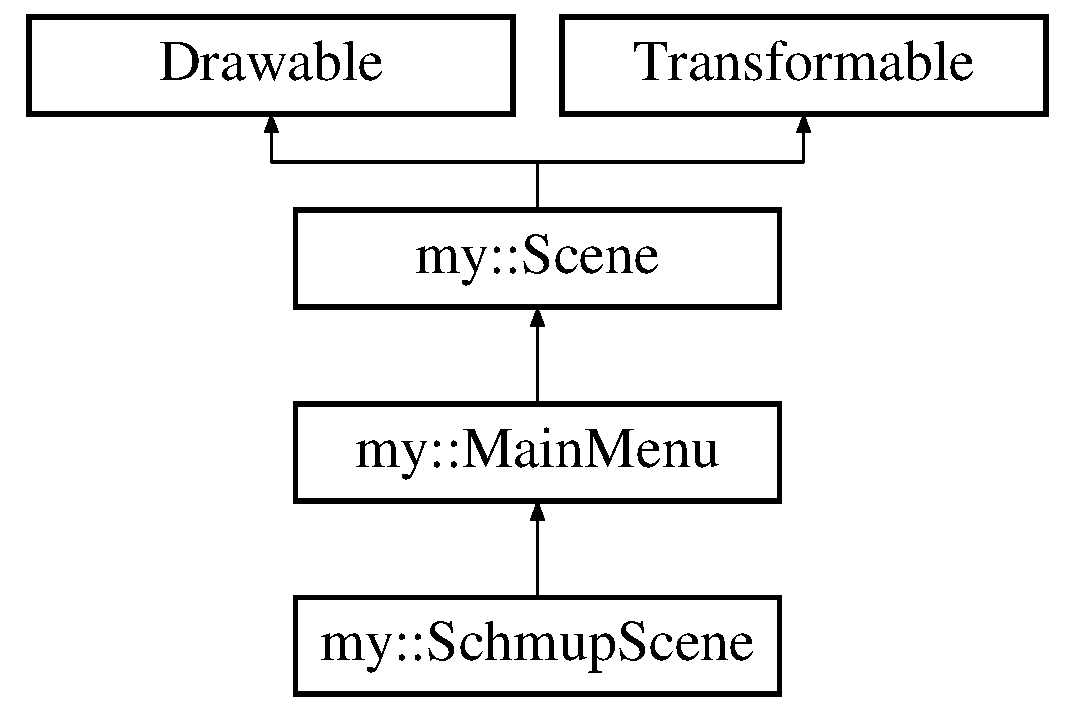
\includegraphics[height=4.000000cm]{classmy_1_1MainMenu}
\end{center}
\end{figure}
\subsection*{Fonctions membres publiques}
\begin{DoxyCompactItemize}
\item 
virtual const \hyperlink{structmy_1_1SceneReturnValue}{Scene\+Return\+Value} \hyperlink{classmy_1_1MainMenu_ada39ad2f51014f08e4526056967daf47}{Update} (sf\+::\+Render\+Window \&window)  throw (std\+::exception)
\begin{DoxyCompactList}\small\item\em Met à jour les différentes entités. \end{DoxyCompactList}\item 
virtual void \hyperlink{classmy_1_1MainMenu_a56e81061a8d8d9a0da77267bd38ec058}{Initialize} (X\+M\+L\+Node\+::\+X\+M\+L\+Node\+Ptr scene\+Root)  throw (std\+::out\+\_\+of\+\_\+range, std\+::invalid\+\_\+argument)
\begin{DoxyCompactList}\small\item\em Initialise les entités. \end{DoxyCompactList}\item 
\mbox{\Hypertarget{classmy_1_1MainMenu_aace3282e435e32542dd3d6ee9bb76ea2}\label{classmy_1_1MainMenu_aace3282e435e32542dd3d6ee9bb76ea2}} 
virtual void \hyperlink{classmy_1_1MainMenu_aace3282e435e32542dd3d6ee9bb76ea2}{Reset} ()  throw (std\+::out\+\_\+of\+\_\+range, std\+::invalid\+\_\+argument)
\begin{DoxyCompactList}\small\item\em Replace les entités à leurs valeur de base. \end{DoxyCompactList}\end{DoxyCompactItemize}
\subsection*{Types protégés}
\begin{DoxyCompactItemize}
\item 
\mbox{\Hypertarget{classmy_1_1MainMenu_a102ed07102cbecf38cf0553175a1256c}\label{classmy_1_1MainMenu_a102ed07102cbecf38cf0553175a1256c}} 
typedef void(Main\+Menu\+::$\ast$ {\bfseries Initialization\+Function}) (X\+M\+L\+Node\+::\+X\+M\+L\+Node\+Ptr)
\item 
\mbox{\Hypertarget{classmy_1_1MainMenu_a10e6c31633e05d88d7b7681fce10a397}\label{classmy_1_1MainMenu_a10e6c31633e05d88d7b7681fce10a397}} 
typedef std\+::pair$<$ std\+::string, Initialization\+Function $>$ {\bfseries Init\+Function\+Pair}
\end{DoxyCompactItemize}
\subsection*{Fonctions membres protégées}
\begin{DoxyCompactItemize}
\item 
\mbox{\Hypertarget{classmy_1_1MainMenu_af378fdb76cb97944ee6b5501933ee669}\label{classmy_1_1MainMenu_af378fdb76cb97944ee6b5501933ee669}} 
void \hyperlink{classmy_1_1MainMenu_af378fdb76cb97944ee6b5501933ee669}{draw} (sf\+::\+Render\+Target \&target, sf\+::\+Render\+States states) const noexcept
\begin{DoxyCompactList}\small\item\em Dessine les entités. \end{DoxyCompactList}\item 
\mbox{\Hypertarget{classmy_1_1MainMenu_a72f1d70bd3785fda568a4eea63c5dafe}\label{classmy_1_1MainMenu_a72f1d70bd3785fda568a4eea63c5dafe}} 
void {\bfseries Initialize\+Functions} () noexcept
\item 
\mbox{\Hypertarget{classmy_1_1MainMenu_a296884bc71735ca403dbf764393da846}\label{classmy_1_1MainMenu_a296884bc71735ca403dbf764393da846}} 
void {\bfseries Initialize\+Cursor} (X\+M\+L\+Node\+::\+X\+M\+L\+Node\+Ptr cursor\+Node)  throw (std\+::out\+\_\+of\+\_\+range, std\+::invalid\+\_\+argument)
\item 
\mbox{\Hypertarget{classmy_1_1MainMenu_ac5788ee93769d1b77d613e5f3755c9ad}\label{classmy_1_1MainMenu_ac5788ee93769d1b77d613e5f3755c9ad}} 
void {\bfseries Initialize\+Background} (X\+M\+L\+Node\+::\+X\+M\+L\+Node\+Ptr background\+Node)  throw (std\+::out\+\_\+of\+\_\+range, std\+::invalid\+\_\+argument)
\item 
\mbox{\Hypertarget{classmy_1_1MainMenu_abfe185e68ceb5392ec2e7a82036f6659}\label{classmy_1_1MainMenu_abfe185e68ceb5392ec2e7a82036f6659}} 
void {\bfseries Initialize\+Panel} (X\+M\+L\+Node\+::\+X\+M\+L\+Node\+Ptr panel\+Node)  throw (std\+::out\+\_\+of\+\_\+range, std\+::invalid\+\_\+argument)
\item 
\mbox{\Hypertarget{classmy_1_1MainMenu_a783a7ca45c020dc4b4774f6c71a034e4}\label{classmy_1_1MainMenu_a783a7ca45c020dc4b4774f6c71a034e4}} 
void {\bfseries Update\+Objects} (sf\+::\+Render\+Window \&window)  throw (std\+::out\+\_\+of\+\_\+range)
\end{DoxyCompactItemize}
\subsection*{Attributs protégés}
\begin{DoxyCompactItemize}
\item 
\mbox{\Hypertarget{classmy_1_1MainMenu_a6353917fac209a9e2b373d0baf8e706d}\label{classmy_1_1MainMenu_a6353917fac209a9e2b373d0baf8e706d}} 
Sprite\+Object\+::\+Sprite\+Object\+Ptr {\bfseries m\+\_\+background}
\item 
\mbox{\Hypertarget{classmy_1_1MainMenu_a7026ad1d5239747cafeb0311bd1be6c3}\label{classmy_1_1MainMenu_a7026ad1d5239747cafeb0311bd1be6c3}} 
std\+::vector$<$ Panel\+::\+Panel\+Ptr $>$ {\bfseries m\+\_\+panels}
\item 
\mbox{\Hypertarget{classmy_1_1MainMenu_a7b4c388904d29dacaed752d24806af07}\label{classmy_1_1MainMenu_a7b4c388904d29dacaed752d24806af07}} 
Cursor\+::\+Cursor\+Ptr {\bfseries m\+\_\+cursor}
\item 
\mbox{\Hypertarget{classmy_1_1MainMenu_a14fa5f4a1d39c3a395421d40ab5e70e1}\label{classmy_1_1MainMenu_a14fa5f4a1d39c3a395421d40ab5e70e1}} 
X\+M\+L\+Node\+::\+X\+M\+L\+Node\+Ptr {\bfseries m\+\_\+root}
\item 
\mbox{\Hypertarget{classmy_1_1MainMenu_ac20c2eeca3ed98c03be2895ed97ffe2f}\label{classmy_1_1MainMenu_ac20c2eeca3ed98c03be2895ed97ffe2f}} 
std\+::vector$<$ Init\+Function\+Pair $>$ {\bfseries m\+\_\+initialization\+Functions}
\end{DoxyCompactItemize}
\subsection*{Attributs protégés statiques}
\begin{DoxyCompactItemize}
\item 
\mbox{\Hypertarget{classmy_1_1MainMenu_a46b0174e3a1c0b4a1900c08a1466f6ee}\label{classmy_1_1MainMenu_a46b0174e3a1c0b4a1900c08a1466f6ee}} 
static const std\+::string {\bfseries S\+C\+E\+N\+E\+\_\+\+C\+U\+R\+S\+O\+R\+\_\+\+N\+O\+DE} = \char`\"{}cursor\char`\"{}
\item 
\mbox{\Hypertarget{classmy_1_1MainMenu_a2b1bd6d21170cf4add1664de523477fd}\label{classmy_1_1MainMenu_a2b1bd6d21170cf4add1664de523477fd}} 
static const std\+::string {\bfseries S\+C\+E\+N\+E\+\_\+\+B\+A\+C\+K\+G\+R\+O\+U\+N\+D\+\_\+\+N\+O\+DE} = \char`\"{}background\char`\"{}
\item 
\mbox{\Hypertarget{classmy_1_1MainMenu_aec125c05b5d2f5d5b93a994d1d44b15b}\label{classmy_1_1MainMenu_aec125c05b5d2f5d5b93a994d1d44b15b}} 
static const std\+::string {\bfseries S\+C\+E\+N\+E\+\_\+\+P\+A\+N\+E\+L\+\_\+\+N\+O\+DE} = \char`\"{}panel\char`\"{}
\end{DoxyCompactItemize}
\subsection*{Membres hérités additionnels}


\subsection{Documentation des fonctions membres}
\mbox{\Hypertarget{classmy_1_1MainMenu_a56e81061a8d8d9a0da77267bd38ec058}\label{classmy_1_1MainMenu_a56e81061a8d8d9a0da77267bd38ec058}} 
\index{my\+::\+Main\+Menu@{my\+::\+Main\+Menu}!Initialize@{Initialize}}
\index{Initialize@{Initialize}!my\+::\+Main\+Menu@{my\+::\+Main\+Menu}}
\subsubsection{\texorpdfstring{Initialize()}{Initialize()}}
{\footnotesize\ttfamily void my\+::\+Main\+Menu\+::\+Initialize (\begin{DoxyParamCaption}\item[{X\+M\+L\+Node\+::\+X\+M\+L\+Node\+Ptr}]{scene\+Root }\end{DoxyParamCaption}) throw  std\+::out\+\_\+of\+\_\+range, std\+::invalid\+\_\+argument) \hspace{0.3cm}{\ttfamily [virtual]}}



Initialise les entités. 

{\bfseries Arguments}~\newline
 scene\+Root\+: Noeud X\+ML contenant les informations sur la scène 

Implémente \hyperlink{classmy_1_1Scene_ac9401c5ec0e8a740fa338324a7df67a6}{my\+::\+Scene}.



Réimplémentée dans \hyperlink{classmy_1_1SchmupScene_ad1febbc7aaf1fc8b2eb4d02cdbf3f57a}{my\+::\+Schmup\+Scene}.

\mbox{\Hypertarget{classmy_1_1MainMenu_ada39ad2f51014f08e4526056967daf47}\label{classmy_1_1MainMenu_ada39ad2f51014f08e4526056967daf47}} 
\index{my\+::\+Main\+Menu@{my\+::\+Main\+Menu}!Update@{Update}}
\index{Update@{Update}!my\+::\+Main\+Menu@{my\+::\+Main\+Menu}}
\subsubsection{\texorpdfstring{Update()}{Update()}}
{\footnotesize\ttfamily const \hyperlink{structmy_1_1SceneReturnValue}{Scene\+Return\+Value} my\+::\+Main\+Menu\+::\+Update (\begin{DoxyParamCaption}\item[{sf\+::\+Render\+Window \&}]{window }\end{DoxyParamCaption}) throw  std\+::exception) \hspace{0.3cm}{\ttfamily [virtual]}}



Met à jour les différentes entités. 

{\bfseries Arguments}~\newline
 window\+: La fenêtre de rendu actuellement utilisé. 

Implémente \hyperlink{classmy_1_1Scene_ae9799de62a6daa9650e040f9f17c78df}{my\+::\+Scene}.



Réimplémentée dans \hyperlink{classmy_1_1SchmupScene_ad07d5b2302f0a4250150d51fdcfa1c0b}{my\+::\+Schmup\+Scene}.



La documentation de cette classe a été générée à partir des fichiers suivants \+:\begin{DoxyCompactItemize}
\item 
includes/my\+\_\+menu\+\_\+lib/Main\+Menu.\+hpp\item 
lib/my\+\_\+menu\+\_\+lib/Main\+Menu.\+cpp\end{DoxyCompactItemize}

\hypertarget{classmy_1_1MessagesException}{}\section{Référence de la classe my\+:\+:Messages\+Exception}
\label{classmy_1_1MessagesException}\index{my\+::\+Messages\+Exception@{my\+::\+Messages\+Exception}}
\subsection*{Fonctions membres publiques statiques}
\begin{DoxyCompactItemize}
\item 
\mbox{\Hypertarget{classmy_1_1MessagesException_a674b0f2037360cef55477d31b81258d6}\label{classmy_1_1MessagesException_a674b0f2037360cef55477d31b81258d6}} 
static const std\+::string {\bfseries Null\+Ptr} (const std\+::string \&function\+Prototype, const std\+::string \&var\+Name) noexcept
\item 
\mbox{\Hypertarget{classmy_1_1MessagesException_a96756489d482f7d0196a3047679a6c7d}\label{classmy_1_1MessagesException_a96756489d482f7d0196a3047679a6c7d}} 
static const std\+::string {\bfseries Invalid\+Index} (const std\+::string \&function\+Prototype, const std\+::string \&var\+Name, int value) noexcept
\item 
\mbox{\Hypertarget{classmy_1_1MessagesException_ad1683b3ea0240b2b7aeddfcc1a2edf17}\label{classmy_1_1MessagesException_ad1683b3ea0240b2b7aeddfcc1a2edf17}} 
static const std\+::string {\bfseries File\+Not\+Found} (const std\+::string \&function\+Prototype, const std\+::string \&file\+Name) noexcept
\item 
\mbox{\Hypertarget{classmy_1_1MessagesException_a3e2aa4d58e6781c9d75373a3e9329666}\label{classmy_1_1MessagesException_a3e2aa4d58e6781c9d75373a3e9329666}} 
static const std\+::string {\bfseries Syntax\+Error} (const std\+::string \&function\+Prototype, const std\+::string \&file\+Name, unsigned line\+Num, unsigned char\+Num, const std\+::string \&error\+Message, const std\+::string \&expected\+Message)
\end{DoxyCompactItemize}


La documentation de cette classe a été générée à partir des fichiers suivants \+:\begin{DoxyCompactItemize}
\item 
includes/my\+\_\+graph\+\_\+lib/Messages\+Exception.\+hpp\item 
lib/my\+\_\+graph\+\_\+lib/Messages\+Exception.\+cpp\end{DoxyCompactItemize}

\hypertarget{classmy_1_1MoovableObject}{}\section{Référence de la classe my\+:\+:Moovable\+Object}
\label{classmy_1_1MoovableObject}\index{my\+::\+Moovable\+Object@{my\+::\+Moovable\+Object}}
Graphe d\textquotesingle{}héritage de my\+:\+:Moovable\+Object\+:\begin{figure}[H]
\begin{center}
\leavevmode
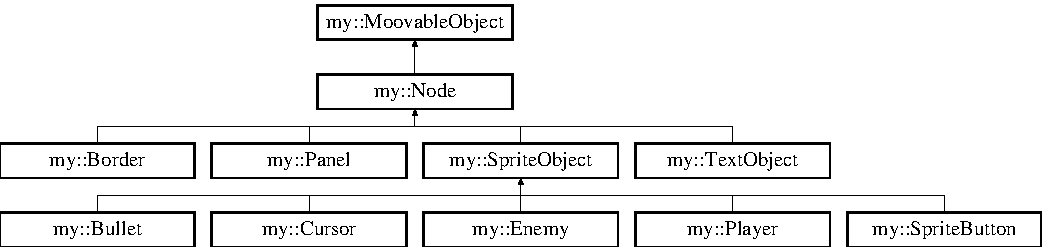
\includegraphics[height=3.318518cm]{classmy_1_1MoovableObject}
\end{center}
\end{figure}
\subsection*{Types publics}
\begin{DoxyCompactItemize}
\item 
\mbox{\Hypertarget{classmy_1_1MoovableObject_a2fd474d748e95a8439e00ac45ce4c419}\label{classmy_1_1MoovableObject_a2fd474d748e95a8439e00ac45ce4c419}} 
typedef std\+::shared\+\_\+ptr$<$ \hyperlink{classmy_1_1MoovableObject}{Moovable\+Object} $>$ {\bfseries Moovable\+Object\+Ptr}
\end{DoxyCompactItemize}
\subsection*{Fonctions membres publiques}
\begin{DoxyCompactItemize}
\item 
\mbox{\Hypertarget{classmy_1_1MoovableObject_a4302b691f78b37b7c316085ed45f7ac9}\label{classmy_1_1MoovableObject_a4302b691f78b37b7c316085ed45f7ac9}} 
void {\bfseries Reset\+Deplacement} ()
\item 
\mbox{\Hypertarget{classmy_1_1MoovableObject_a5df53e0f738ed579d60fd177d1a5d536}\label{classmy_1_1MoovableObject_a5df53e0f738ed579d60fd177d1a5d536}} 
void {\bfseries Clear\+Deplacement} ()
\item 
\mbox{\Hypertarget{classmy_1_1MoovableObject_ad3d84238f50e6a0fb50b8e91c55a9f23}\label{classmy_1_1MoovableObject_ad3d84238f50e6a0fb50b8e91c55a9f23}} 
bool {\bfseries Is\+On\+Deplacement} () const noexcept
\item 
\mbox{\Hypertarget{classmy_1_1MoovableObject_aa74659c36cf79efa1e8ef68485e0b240}\label{classmy_1_1MoovableObject_aa74659c36cf79efa1e8ef68485e0b240}} 
bool {\bfseries Can\+Move} () const noexcept
\item 
\mbox{\Hypertarget{classmy_1_1MoovableObject_a0da6d199a21b7bd02b744e73f0ba9db2}\label{classmy_1_1MoovableObject_a0da6d199a21b7bd02b744e73f0ba9db2}} 
float {\bfseries Get\+Speed} () const noexcept
\item 
\mbox{\Hypertarget{classmy_1_1MoovableObject_a29752f95b08d211af58337468cfa00ac}\label{classmy_1_1MoovableObject_a29752f95b08d211af58337468cfa00ac}} 
const sf\+::\+Vector2f \& {\bfseries Get\+Direction} () const noexcept
\item 
\mbox{\Hypertarget{classmy_1_1MoovableObject_a38ed98b7521553a560426dd9ca19c1b0}\label{classmy_1_1MoovableObject_a38ed98b7521553a560426dd9ca19c1b0}} 
int {\bfseries Get\+Frame\+Rate} () const noexcept
\item 
\mbox{\Hypertarget{classmy_1_1MoovableObject_a4a1c2fa789043425bc0aa5d276788a89}\label{classmy_1_1MoovableObject_a4a1c2fa789043425bc0aa5d276788a89}} 
int {\bfseries Get\+Deplacememt\+Rate} () const noexcept
\item 
\mbox{\Hypertarget{classmy_1_1MoovableObject_abfad2bb10fec55f3a2d1e3f371ce6259}\label{classmy_1_1MoovableObject_abfad2bb10fec55f3a2d1e3f371ce6259}} 
int {\bfseries Get\+Deplacement\+Repetition} () const noexcept
\item 
\mbox{\Hypertarget{classmy_1_1MoovableObject_ad248f892b458765604e3f9832a60c146}\label{classmy_1_1MoovableObject_ad248f892b458765604e3f9832a60c146}} 
int {\bfseries Get\+Repetition\+Max} () const noexcept
\item 
\mbox{\Hypertarget{classmy_1_1MoovableObject_aa968bbaf7ab53cd586f1608c578bebf0}\label{classmy_1_1MoovableObject_aa968bbaf7ab53cd586f1608c578bebf0}} 
sf\+::\+Vector2f $\ast$ {\bfseries Get\+Target} () const noexcept
\item 
\mbox{\Hypertarget{classmy_1_1MoovableObject_ab16c059fa42967679b4f6a3608c0cc70}\label{classmy_1_1MoovableObject_ab16c059fa42967679b4f6a3608c0cc70}} 
void {\bfseries Set\+On\+Deplacement} (bool on\+Deplacement) noexcept
\item 
\mbox{\Hypertarget{classmy_1_1MoovableObject_a88156d7514b00250efe0dacae22c1081}\label{classmy_1_1MoovableObject_a88156d7514b00250efe0dacae22c1081}} 
void {\bfseries Set\+Speed} (float speed) noexcept
\item 
\mbox{\Hypertarget{classmy_1_1MoovableObject_a715e0bc98cd76d55b349cc7b3576b2a2}\label{classmy_1_1MoovableObject_a715e0bc98cd76d55b349cc7b3576b2a2}} 
void {\bfseries Set\+Direction} (const sf\+::\+Vector2f \&direction) noexcept
\item 
\mbox{\Hypertarget{classmy_1_1MoovableObject_ab321cbf7f36daf3cbcc7d64c8ffd76d6}\label{classmy_1_1MoovableObject_ab321cbf7f36daf3cbcc7d64c8ffd76d6}} 
void {\bfseries Set\+Frame\+Rate} (int frame\+Rate) noexcept
\item 
\mbox{\Hypertarget{classmy_1_1MoovableObject_aaded98ee5e816f3625f7c8131e39e379}\label{classmy_1_1MoovableObject_aaded98ee5e816f3625f7c8131e39e379}} 
void {\bfseries Set\+Deplacement\+Rate} (int deplacement\+Rate) noexcept
\item 
\mbox{\Hypertarget{classmy_1_1MoovableObject_a7b57191d3cdbe81551a5947af184ca40}\label{classmy_1_1MoovableObject_a7b57191d3cdbe81551a5947af184ca40}} 
void {\bfseries Set\+Deplacement\+Repetition} (int deplacement\+Repetition) noexcept
\item 
\mbox{\Hypertarget{classmy_1_1MoovableObject_a50f93ff5d9816b85275e2a65874ac7e9}\label{classmy_1_1MoovableObject_a50f93ff5d9816b85275e2a65874ac7e9}} 
void {\bfseries Set\+Repetition\+Max} (int repetition\+Max) noexcept
\item 
\mbox{\Hypertarget{classmy_1_1MoovableObject_a85beb58fdd3f22e3a110cc1ef15f58e2}\label{classmy_1_1MoovableObject_a85beb58fdd3f22e3a110cc1ef15f58e2}} 
void {\bfseries Set\+Target} (sf\+::\+Vector2f $\ast$target) noexcept
\end{DoxyCompactItemize}
\subsection*{Fonctions membres protégées}
\begin{DoxyCompactItemize}
\item 
\mbox{\Hypertarget{classmy_1_1MoovableObject_a805a7e19ec70558728f0467a9e05651a}\label{classmy_1_1MoovableObject_a805a7e19ec70558728f0467a9e05651a}} 
virtual void {\bfseries Update\+Movement} ()
\end{DoxyCompactItemize}
\subsection*{Attributs protégés}
\begin{DoxyCompactItemize}
\item 
\mbox{\Hypertarget{classmy_1_1MoovableObject_a56364bb6ed487aefb33b12ea4ce4ae4f}\label{classmy_1_1MoovableObject_a56364bb6ed487aefb33b12ea4ce4ae4f}} 
bool {\bfseries m\+\_\+on\+Deplacement}
\item 
\mbox{\Hypertarget{classmy_1_1MoovableObject_aa8457f2cbc937965ddd9c577560ea75c}\label{classmy_1_1MoovableObject_aa8457f2cbc937965ddd9c577560ea75c}} 
bool {\bfseries m\+\_\+can\+Move}
\item 
\mbox{\Hypertarget{classmy_1_1MoovableObject_a290ccefafadf9a0ca24db7a0a91bdc46}\label{classmy_1_1MoovableObject_a290ccefafadf9a0ca24db7a0a91bdc46}} 
float {\bfseries m\+\_\+speed}
\item 
\mbox{\Hypertarget{classmy_1_1MoovableObject_a93dfa01e2a5b853bd28edfd2b5f72b5f}\label{classmy_1_1MoovableObject_a93dfa01e2a5b853bd28edfd2b5f72b5f}} 
sf\+::\+Vector2f {\bfseries m\+\_\+direction}
\item 
\mbox{\Hypertarget{classmy_1_1MoovableObject_a9ef9e4b79fae2447d36518155f6b8e54}\label{classmy_1_1MoovableObject_a9ef9e4b79fae2447d36518155f6b8e54}} 
int {\bfseries m\+\_\+frame\+Rate}
\item 
\mbox{\Hypertarget{classmy_1_1MoovableObject_a4a02ffbb4f66d72f39f2106281e4f3a7}\label{classmy_1_1MoovableObject_a4a02ffbb4f66d72f39f2106281e4f3a7}} 
int {\bfseries m\+\_\+deplacement\+Rate}
\item 
\mbox{\Hypertarget{classmy_1_1MoovableObject_a5f5ead094141e29bf7f0251a0b780059}\label{classmy_1_1MoovableObject_a5f5ead094141e29bf7f0251a0b780059}} 
int {\bfseries m\+\_\+deplacement\+Repetition}
\item 
\mbox{\Hypertarget{classmy_1_1MoovableObject_a264d9d3a9c16fd1435c6b48bca23b7a8}\label{classmy_1_1MoovableObject_a264d9d3a9c16fd1435c6b48bca23b7a8}} 
int {\bfseries m\+\_\+repetition\+Max}
\item 
\mbox{\Hypertarget{classmy_1_1MoovableObject_a6402bb1ad6cfa59483d9eb70f4ad1aab}\label{classmy_1_1MoovableObject_a6402bb1ad6cfa59483d9eb70f4ad1aab}} 
sf\+::\+Vector2f $\ast$ {\bfseries m\+\_\+target}
\end{DoxyCompactItemize}


La documentation de cette classe a été générée à partir des fichiers suivants \+:\begin{DoxyCompactItemize}
\item 
includes/my\+\_\+graph\+\_\+lib/Moovable\+Object.\+hpp\item 
lib/my\+\_\+graph\+\_\+lib/Moovable\+Object.\+cpp\end{DoxyCompactItemize}

\hypertarget{classmy_1_1Node}{}\section{Référence de la classe my\+:\+:Node}
\label{classmy_1_1Node}\index{my\+::\+Node@{my\+::\+Node}}
Graphe d\textquotesingle{}héritage de my\+:\+:Node\+:\begin{figure}[H]
\begin{center}
\leavevmode
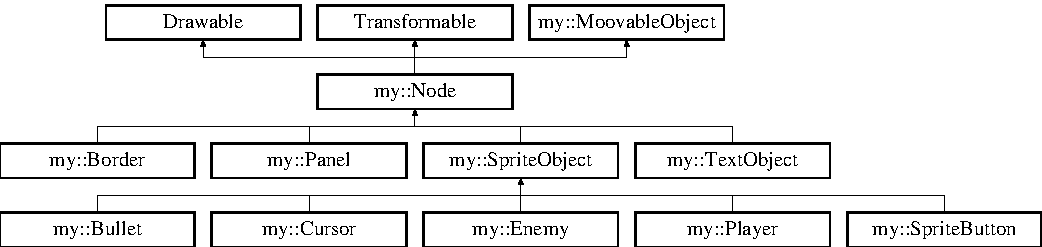
\includegraphics[height=3.318518cm]{classmy_1_1Node}
\end{center}
\end{figure}
\subsection*{Types publics}
\begin{DoxyCompactItemize}
\item 
\mbox{\Hypertarget{classmy_1_1Node_a84da714a586798cd894654ca825e0211}\label{classmy_1_1Node_a84da714a586798cd894654ca825e0211}} 
typedef std\+::shared\+\_\+ptr$<$ \hyperlink{classmy_1_1Node}{Node} $>$ {\bfseries Node\+Ptr}
\item 
\mbox{\Hypertarget{classmy_1_1Node_a6232a3681184c2ed92028994c619bcf6}\label{classmy_1_1Node_a6232a3681184c2ed92028994c619bcf6}} 
typedef std\+::list$<$ Node\+Ptr $>$ {\bfseries Node\+List}
\end{DoxyCompactItemize}
\subsection*{Fonctions membres publiques}
\begin{DoxyCompactItemize}
\item 
\mbox{\Hypertarget{classmy_1_1Node_afe43c3936b45ba018babfae34dd08820}\label{classmy_1_1Node_afe43c3936b45ba018babfae34dd08820}} 
virtual void {\bfseries Update} ()
\item 
\mbox{\Hypertarget{classmy_1_1Node_aa57a107fbe9dae93903ea5799ffe8712}\label{classmy_1_1Node_aa57a107fbe9dae93903ea5799ffe8712}} 
Node\+List {\bfseries Get\+Childs} () const noexcept
\item 
\mbox{\Hypertarget{classmy_1_1Node_a44d827884d796d63c0becfc9adbefd3e}\label{classmy_1_1Node_a44d827884d796d63c0becfc9adbefd3e}} 
bool {\bfseries Is\+Visible} () const noexcept
\item 
\mbox{\Hypertarget{classmy_1_1Node_ac7972cd7d8bd9eb2757a94b6ab62072a}\label{classmy_1_1Node_ac7972cd7d8bd9eb2757a94b6ab62072a}} 
virtual bool {\bfseries Is\+Intersect} (const sf\+::\+Vector2f \&point) const noexcept=0
\item 
\mbox{\Hypertarget{classmy_1_1Node_a3e5b63c91ce28392d64ce73c15b02ee0}\label{classmy_1_1Node_a3e5b63c91ce28392d64ce73c15b02ee0}} 
virtual bool {\bfseries Is\+Intersect} (const sf\+::\+Float\+Rect \&square) const noexcept=0
\item 
\mbox{\Hypertarget{classmy_1_1Node_aed8cff06c09cf7fd8a1bd38212572930}\label{classmy_1_1Node_aed8cff06c09cf7fd8a1bd38212572930}} 
virtual const sf\+::\+Float\+Rect {\bfseries Get\+Hit\+Box} () const noexcept=0
\item 
\mbox{\Hypertarget{classmy_1_1Node_ab687559c87eff28cd097f4fe0b3369a2}\label{classmy_1_1Node_ab687559c87eff28cd097f4fe0b3369a2}} 
void {\bfseries Add\+Child} (Node\+Ptr new\+Child)  throw (std\+::invalid\+\_\+argument)
\item 
\mbox{\Hypertarget{classmy_1_1Node_a181cca5f4782bd73ecdfceb57e93994a}\label{classmy_1_1Node_a181cca5f4782bd73ecdfceb57e93994a}} 
void {\bfseries Add\+Childs} (Node\+List new\+Childs)  throw (std\+::invalid\+\_\+argument)
\item 
\mbox{\Hypertarget{classmy_1_1Node_a096398315abb0abddc553a13dfefa5ca}\label{classmy_1_1Node_a096398315abb0abddc553a13dfefa5ca}} 
void {\bfseries Set\+Visible} (bool visible) noexcept
\end{DoxyCompactItemize}
\subsection*{Fonctions membres protégées}
\begin{DoxyCompactItemize}
\item 
\mbox{\Hypertarget{classmy_1_1Node_a71ddeab220702a1329e436d890ba5c19}\label{classmy_1_1Node_a71ddeab220702a1329e436d890ba5c19}} 
virtual void {\bfseries draw} (sf\+::\+Render\+Target \&target, sf\+::\+Render\+States states) const
\item 
\mbox{\Hypertarget{classmy_1_1Node_a70cf326c23afe568d5f450c0217258c0}\label{classmy_1_1Node_a70cf326c23afe568d5f450c0217258c0}} 
virtual void {\bfseries Update\+Movement} () noexcept
\end{DoxyCompactItemize}
\subsection*{Attributs protégés}
\begin{DoxyCompactItemize}
\item 
\mbox{\Hypertarget{classmy_1_1Node_a4b1e064d05cefffda0ce6bae3193f4d0}\label{classmy_1_1Node_a4b1e064d05cefffda0ce6bae3193f4d0}} 
Node\+List {\bfseries m\+\_\+childs}
\item 
\mbox{\Hypertarget{classmy_1_1Node_a1d55e20d5b5ab37c5e8b3c0b84af011f}\label{classmy_1_1Node_a1d55e20d5b5ab37c5e8b3c0b84af011f}} 
bool {\bfseries m\+\_\+visible}
\end{DoxyCompactItemize}
\subsection*{Attributs protégés statiques}
\begin{DoxyCompactItemize}
\item 
\mbox{\Hypertarget{classmy_1_1Node_a80d18cd003826c77e7c2ef769dd7dc3a}\label{classmy_1_1Node_a80d18cd003826c77e7c2ef769dd7dc3a}} 
static const std\+::string {\bfseries M\+O\+O\+V\+I\+N\+G\+\_\+\+A\+N\+I\+M\+\_\+\+N\+A\+ME} = \char`\"{}move\char`\"{}
\end{DoxyCompactItemize}


La documentation de cette classe a été générée à partir des fichiers suivants \+:\begin{DoxyCompactItemize}
\item 
includes/my\+\_\+graph\+\_\+lib/Node.\+hpp\item 
lib/my\+\_\+graph\+\_\+lib/Node.\+cpp\end{DoxyCompactItemize}

\hypertarget{classmy_1_1ObjectPool}{}\section{Référence de la classe my\+:\+:Object\+Pool}
\label{classmy_1_1ObjectPool}\index{my\+::\+Object\+Pool@{my\+::\+Object\+Pool}}
\subsection*{Fonctions membres publiques statiques}
\begin{DoxyCompactItemize}
\item 
\mbox{\Hypertarget{classmy_1_1ObjectPool_a998c84ca9082a40422a96c83c928af4a}\label{classmy_1_1ObjectPool_a998c84ca9082a40422a96c83c928af4a}} 
static Sprite\+Object\+::\+Sprite\+Object\+Ptr {\bfseries Create\+Sprite} (X\+M\+L\+Node\+::\+X\+M\+L\+Node\+Ptr sprite\+Node)  throw (std\+::out\+\_\+of\+\_\+range, std\+::invalid\+\_\+argument)
\item 
\mbox{\Hypertarget{classmy_1_1ObjectPool_a8795fd18ec08dcdb060095126843764e}\label{classmy_1_1ObjectPool_a8795fd18ec08dcdb060095126843764e}} 
static Text\+Object\+::\+Text\+Object\+Ptr {\bfseries Create\+Text} (X\+M\+L\+Node\+::\+X\+M\+L\+Node\+Ptr text\+Node)  throw (std\+::out\+\_\+of\+\_\+range, std\+::invalid\+\_\+argument)
\item 
\mbox{\Hypertarget{classmy_1_1ObjectPool_a6aee2d2951142a5691fc9ef33f3c8c47}\label{classmy_1_1ObjectPool_a6aee2d2951142a5691fc9ef33f3c8c47}} 
static Border\+::\+Border\+Ptr {\bfseries Create\+Border} (X\+M\+L\+Node\+::\+X\+M\+L\+Node\+Ptr border\+Node)  throw (std\+::out\+\_\+of\+\_\+range, std\+::invalid\+\_\+argument)
\item 
\mbox{\Hypertarget{classmy_1_1ObjectPool_ae05dd9c86ea759f3a8593c5330e23786}\label{classmy_1_1ObjectPool_ae05dd9c86ea759f3a8593c5330e23786}} 
static Panel\+::\+Panel\+Ptr {\bfseries Create\+Panel} (X\+M\+L\+Node\+::\+X\+M\+L\+Node\+Ptr panel\+Node)  throw (std\+::out\+\_\+of\+\_\+range, std\+::invalid\+\_\+argument)
\item 
\mbox{\Hypertarget{classmy_1_1ObjectPool_a63ddc3d83766c1d3dbbe1120ce335abe}\label{classmy_1_1ObjectPool_a63ddc3d83766c1d3dbbe1120ce335abe}} 
static Cursor\+::\+Cursor\+Ptr {\bfseries Create\+Cursor} (X\+M\+L\+Node\+::\+X\+M\+L\+Node\+Ptr cursor\+Node)  throw (std\+::out\+\_\+of\+\_\+range, std\+::invalid\+\_\+argument)
\item 
\mbox{\Hypertarget{classmy_1_1ObjectPool_a7e8e80d52717c9b972b16007ed73658a}\label{classmy_1_1ObjectPool_a7e8e80d52717c9b972b16007ed73658a}} 
static Sprite\+Button\+::\+Sprite\+Button\+Ptr {\bfseries Create\+Sprite\+Button} (X\+M\+L\+Node\+::\+X\+M\+L\+Node\+Ptr sprite\+Button\+Node)  throw (std\+::out\+\_\+of\+\_\+range, std\+::invalid\+\_\+argument)
\item 
\mbox{\Hypertarget{classmy_1_1ObjectPool_a8ec76923583ccd1dc344982344fc1eca}\label{classmy_1_1ObjectPool_a8ec76923583ccd1dc344982344fc1eca}} 
static Player\+::\+Player\+Ptr {\bfseries Create\+Player} (X\+M\+L\+Node\+::\+X\+M\+L\+Node\+Ptr player\+Node)  throw (std\+::out\+\_\+of\+\_\+range, std\+::invalid\+\_\+argument)
\item 
\mbox{\Hypertarget{classmy_1_1ObjectPool_a62c813dde06c27493091bd853f6f6cd8}\label{classmy_1_1ObjectPool_a62c813dde06c27493091bd853f6f6cd8}} 
static Enemy\+::\+Enemy\+Ptr {\bfseries Create\+Enemy} (X\+M\+L\+Node\+::\+X\+M\+L\+Node\+Ptr enemy\+Node)  throw (std\+::out\+\_\+of\+\_\+range, std\+::invalid\+\_\+argument)
\item 
\mbox{\Hypertarget{classmy_1_1ObjectPool_a24c54c3d8012d2faea51b360cd5f4a46}\label{classmy_1_1ObjectPool_a24c54c3d8012d2faea51b360cd5f4a46}} 
static Bullet\+::\+Bullet\+Ptr {\bfseries Create\+Bullet} (X\+M\+L\+Node\+::\+X\+M\+L\+Node\+Ptr bullet\+Node)  throw (std\+::out\+\_\+of\+\_\+range, std\+::invalid\+\_\+argument)
\item 
\mbox{\Hypertarget{classmy_1_1ObjectPool_a75da7062dfe02748a2193cf7236e63a3}\label{classmy_1_1ObjectPool_a75da7062dfe02748a2193cf7236e63a3}} 
static sf\+::\+Keyboard\+::\+Key {\bfseries Str\+To\+Input} (const std\+::string \&str)  throw (std\+::invalid\+\_\+argument)
\item 
\mbox{\Hypertarget{classmy_1_1ObjectPool_ad5f86669f0e3e8b93a897ff3d1723cd4}\label{classmy_1_1ObjectPool_ad5f86669f0e3e8b93a897ff3d1723cd4}} 
static Direction {\bfseries Str\+To\+Direction} (const std\+::string \&str)  throw (std\+::invalid\+\_\+argument)
\end{DoxyCompactItemize}


La documentation de cette classe a été générée à partir des fichiers suivants \+:\begin{DoxyCompactItemize}
\item 
includes/my\+\_\+objects\+\_\+lib/Object\+Pool.\+hpp\item 
lib/my\+\_\+objects\+\_\+lib/Object\+Pool.\+cpp\end{DoxyCompactItemize}

\hypertarget{classmy_1_1OperationEvaluator}{}\section{Référence du modèle de la classe my\+:\+:Operation\+Evaluator$<$ T $>$}
\label{classmy_1_1OperationEvaluator}\index{my\+::\+Operation\+Evaluator$<$ T $>$@{my\+::\+Operation\+Evaluator$<$ T $>$}}
\subsection*{Fonctions membres publiques statiques}
\begin{DoxyCompactItemize}
\item 
\mbox{\Hypertarget{classmy_1_1OperationEvaluator_aa9bb54881bfe3734ae5e4da71d013a6e}\label{classmy_1_1OperationEvaluator_aa9bb54881bfe3734ae5e4da71d013a6e}} 
static T {\bfseries Parse\+Operation} (const std\+::string \&operation)  throw (std\+::invalid\+\_\+argument)
\end{DoxyCompactItemize}


La documentation de cette classe a été générée à partir du fichier suivant \+:\begin{DoxyCompactItemize}
\item 
includes/my\+\_\+graph\+\_\+lib/Operation\+Evaluator.\+hpp\end{DoxyCompactItemize}

\hypertarget{classmy_1_1Panel}{}\section{Référence de la classe my\+:\+:Panel}
\label{classmy_1_1Panel}\index{my\+::\+Panel@{my\+::\+Panel}}
Graphe d\textquotesingle{}héritage de my\+:\+:Panel\+:\begin{figure}[H]
\begin{center}
\leavevmode
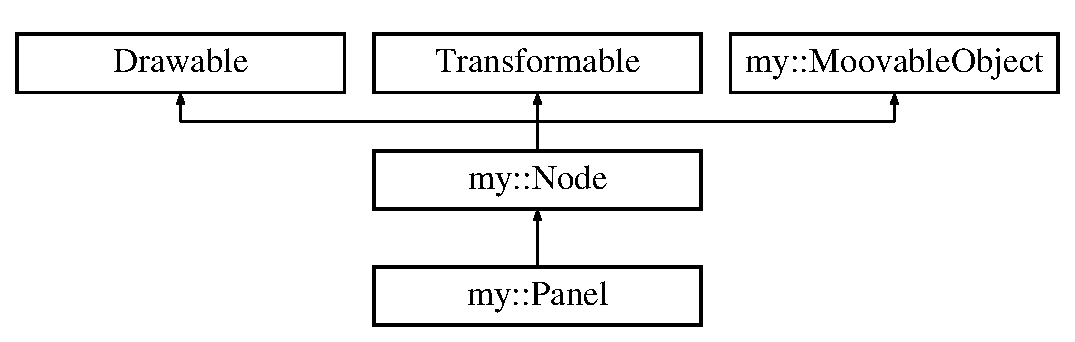
\includegraphics[height=3.000000cm]{classmy_1_1Panel}
\end{center}
\end{figure}
\subsection*{Types publics}
\begin{DoxyCompactItemize}
\item 
\mbox{\Hypertarget{classmy_1_1Panel_a4d8b8e5938fc6636a86c827f9d0ca4c3}\label{classmy_1_1Panel_a4d8b8e5938fc6636a86c827f9d0ca4c3}} 
typedef std\+::shared\+\_\+ptr$<$ \hyperlink{classmy_1_1Panel}{Panel} $>$ {\bfseries Panel\+Ptr}
\item 
\mbox{\Hypertarget{classmy_1_1Panel_a564d9679b0bab4d97778142540ef34ea}\label{classmy_1_1Panel_a564d9679b0bab4d97778142540ef34ea}} 
typedef Sprite\+Button\+::\+Sprite\+Button\+Ptr {\bfseries Panel\+Sprite\+Button}
\item 
\mbox{\Hypertarget{classmy_1_1Panel_ab8c92a11eb9757509f10e9cd6119f68c}\label{classmy_1_1Panel_ab8c92a11eb9757509f10e9cd6119f68c}} 
typedef Text\+Object\+::\+Text\+Object\+Ptr {\bfseries Text\+Button}
\item 
\mbox{\Hypertarget{classmy_1_1Panel_a8b61d17b51fc11dc34c446214ff959c3}\label{classmy_1_1Panel_a8b61d17b51fc11dc34c446214ff959c3}} 
typedef std\+::vector$<$ Panel\+Sprite\+Button $>$ {\bfseries Sprite\+Buttons}
\item 
\mbox{\Hypertarget{classmy_1_1Panel_aa1a364d3ab63a94e52527d3474e34d9e}\label{classmy_1_1Panel_aa1a364d3ab63a94e52527d3474e34d9e}} 
typedef std\+::vector$<$ Text\+Button $>$ {\bfseries Text\+Buttons}
\end{DoxyCompactItemize}
\subsection*{Fonctions membres publiques}
\begin{DoxyCompactItemize}
\item 
\mbox{\Hypertarget{classmy_1_1Panel_aeb4c2641fffa7463155b0f02a569605e}\label{classmy_1_1Panel_aeb4c2641fffa7463155b0f02a569605e}} 
virtual bool {\bfseries Is\+Intersect} (const sf\+::\+Vector2f \&point) const noexcept
\item 
\mbox{\Hypertarget{classmy_1_1Panel_a4550d5dbb1372c550d8b8a04d93d8957}\label{classmy_1_1Panel_a4550d5dbb1372c550d8b8a04d93d8957}} 
virtual bool {\bfseries Is\+Intersect} (const sf\+::\+Float\+Rect \&square) const noexcept
\item 
\mbox{\Hypertarget{classmy_1_1Panel_a38b845449682c439accb6b43c8cbb11c}\label{classmy_1_1Panel_a38b845449682c439accb6b43c8cbb11c}} 
virtual const sf\+::\+Float\+Rect {\bfseries Get\+Hit\+Box} () const noexcept
\item 
\mbox{\Hypertarget{classmy_1_1Panel_a12e5e481395820c64aaa4cb3858638ad}\label{classmy_1_1Panel_a12e5e481395820c64aaa4cb3858638ad}} 
Sprite\+Object\+::\+Sprite\+Object\+Ptr {\bfseries Get\+Background} () const noexcept
\item 
\mbox{\Hypertarget{classmy_1_1Panel_a145142192e283b5581485a81de5ec009}\label{classmy_1_1Panel_a145142192e283b5581485a81de5ec009}} 
Border\+::\+Border\+Ptr {\bfseries Get\+Border} () const noexcept
\item 
\mbox{\Hypertarget{classmy_1_1Panel_a4e76064b1f66de5ac2a671f8b6d6c608}\label{classmy_1_1Panel_a4e76064b1f66de5ac2a671f8b6d6c608}} 
Text\+Object\+::\+Text\+Object\+Ptr {\bfseries Get\+Title} () const noexcept
\item 
\mbox{\Hypertarget{classmy_1_1Panel_abc0b2f1bd63e3f924e02f6795c7d219d}\label{classmy_1_1Panel_abc0b2f1bd63e3f924e02f6795c7d219d}} 
const Sprite\+Buttons \& {\bfseries Get\+Sprite\+Buttons} () const noexcept
\item 
\mbox{\Hypertarget{classmy_1_1Panel_a7ebb1743164a0538c2debcb48553b185}\label{classmy_1_1Panel_a7ebb1743164a0538c2debcb48553b185}} 
const Text\+Buttons \& {\bfseries Get\+Text\+Buttons} () const noexcept
\item 
\mbox{\Hypertarget{classmy_1_1Panel_a6bc042f2ac2d4b4556815eeac005610e}\label{classmy_1_1Panel_a6bc042f2ac2d4b4556815eeac005610e}} 
void {\bfseries Set\+Background} (Sprite\+Object\+::\+Sprite\+Object\+Ptr background) noexcept
\item 
\mbox{\Hypertarget{classmy_1_1Panel_a040474d4d94619dc3f38be0210704fe5}\label{classmy_1_1Panel_a040474d4d94619dc3f38be0210704fe5}} 
void {\bfseries Set\+Border} (Border\+::\+Border\+Ptr border) noexcept
\item 
\mbox{\Hypertarget{classmy_1_1Panel_a04b1f6f32550c35620140526c2242da4}\label{classmy_1_1Panel_a04b1f6f32550c35620140526c2242da4}} 
void {\bfseries Set\+Title} (Text\+Object\+::\+Text\+Object\+Ptr title) noexcept
\item 
\mbox{\Hypertarget{classmy_1_1Panel_a1631e0c015ceca7bd69550fed6aa436b}\label{classmy_1_1Panel_a1631e0c015ceca7bd69550fed6aa436b}} 
void {\bfseries Set\+Sprite\+Buttons} (const Sprite\+Buttons \&buttons) noexcept
\item 
\mbox{\Hypertarget{classmy_1_1Panel_aa8ae6f08a24293d0251c5a787f66cf04}\label{classmy_1_1Panel_aa8ae6f08a24293d0251c5a787f66cf04}} 
void {\bfseries Add\+Sprite\+Button} (const Panel\+Sprite\+Button \&new\+Button) noexcept
\item 
\mbox{\Hypertarget{classmy_1_1Panel_a5cf0eb71b153928290fa38883bf2212d}\label{classmy_1_1Panel_a5cf0eb71b153928290fa38883bf2212d}} 
void {\bfseries Set\+Text\+Buttons} (const Text\+Buttons \&buttons) noexcept
\item 
\mbox{\Hypertarget{classmy_1_1Panel_aae60e439501dabbea7e4737518172411}\label{classmy_1_1Panel_aae60e439501dabbea7e4737518172411}} 
void {\bfseries Add\+Text\+Button} (const Text\+Button \&new\+Button) noexcept
\item 
\mbox{\Hypertarget{classmy_1_1Panel_aaeb58913cdea3605880819f9afe4565a}\label{classmy_1_1Panel_aaeb58913cdea3605880819f9afe4565a}} 
void {\bfseries Update} (const sf\+::\+Vector2f \&mouse\+Pos) noexcept
\end{DoxyCompactItemize}
\subsection*{Membres hérités additionnels}


La documentation de cette classe a été générée à partir des fichiers suivants \+:\begin{DoxyCompactItemize}
\item 
includes/my\+\_\+objects\+\_\+lib/Panel.\+hpp\item 
lib/my\+\_\+objects\+\_\+lib/Panel.\+cpp\end{DoxyCompactItemize}

\hypertarget{classmy_1_1Player}{}\section{Référence de la classe my\+:\+:Player}
\label{classmy_1_1Player}\index{my\+::\+Player@{my\+::\+Player}}
Graphe d\textquotesingle{}héritage de my\+:\+:Player\+:\begin{figure}[H]
\begin{center}
\leavevmode
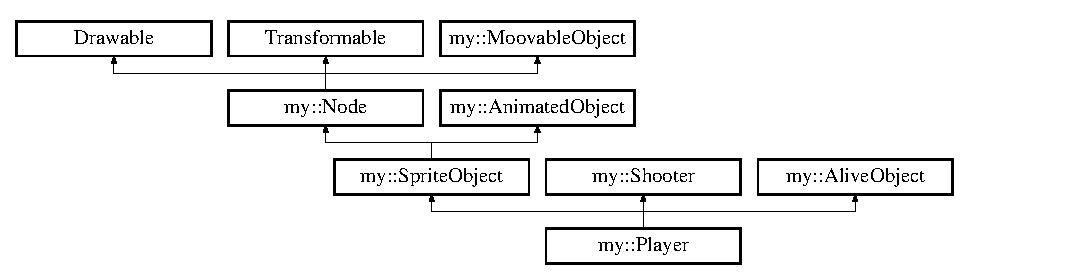
\includegraphics[height=3.318518cm]{classmy_1_1Player}
\end{center}
\end{figure}
\subsection*{Types publics}
\begin{DoxyCompactItemize}
\item 
\mbox{\Hypertarget{classmy_1_1Player_a91ad09d3d6b0e72ad589e7b95f521497}\label{classmy_1_1Player_a91ad09d3d6b0e72ad589e7b95f521497}} 
typedef std\+::shared\+\_\+ptr$<$ \hyperlink{classmy_1_1Player}{Player} $>$ {\bfseries Player\+Ptr}
\item 
\mbox{\Hypertarget{classmy_1_1Player_a4f73979cf1696c825c30744d8c0c4dcc}\label{classmy_1_1Player_a4f73979cf1696c825c30744d8c0c4dcc}} 
typedef std\+::pair$<$ sf\+::\+Keyboard\+::\+Key, Direction $>$ {\bfseries Input\+Deplacement}
\item 
\mbox{\Hypertarget{classmy_1_1Player_a5f7aa685cb5a2660de108f52d44909d5}\label{classmy_1_1Player_a5f7aa685cb5a2660de108f52d44909d5}} 
typedef std\+::pair$<$ sf\+::\+Keyboard\+::\+Key, std\+::string $>$ {\bfseries Input\+Shoot}
\item 
\mbox{\Hypertarget{classmy_1_1Player_a429264ee8d5e72d162ad2b487117cd30}\label{classmy_1_1Player_a429264ee8d5e72d162ad2b487117cd30}} 
typedef std\+::vector$<$ Input\+Deplacement $>$ {\bfseries Inputs\+Deplacement\+List}
\item 
\mbox{\Hypertarget{classmy_1_1Player_a01cba57770a69e897411dba348b9157a}\label{classmy_1_1Player_a01cba57770a69e897411dba348b9157a}} 
typedef std\+::vector$<$ Input\+Shoot $>$ {\bfseries Inputs\+Shoot\+List}
\end{DoxyCompactItemize}
\subsection*{Fonctions membres publiques}
\begin{DoxyCompactItemize}
\item 
\mbox{\Hypertarget{classmy_1_1Player_a820feb1a40c3deba61cbdc071ac9cb86}\label{classmy_1_1Player_a820feb1a40c3deba61cbdc071ac9cb86}} 
virtual void {\bfseries Update} ()  throw (std\+::out\+\_\+of\+\_\+range)
\item 
\mbox{\Hypertarget{classmy_1_1Player_ac438258671e2f52e919504f6f20618c6}\label{classmy_1_1Player_ac438258671e2f52e919504f6f20618c6}} 
const Inputs\+Deplacement\+List \& {\bfseries Get\+Inputs\+Deplacement\+List} () const noexcept
\item 
\mbox{\Hypertarget{classmy_1_1Player_a7bb88e90838652f3783bacf974db3629}\label{classmy_1_1Player_a7bb88e90838652f3783bacf974db3629}} 
const Inputs\+Shoot\+List \& {\bfseries Get\+Inputs\+Shoot\+List} () const noexcept
\item 
\mbox{\Hypertarget{classmy_1_1Player_ab009b7c70c71bd7521583412db111c97}\label{classmy_1_1Player_ab009b7c70c71bd7521583412db111c97}} 
void {\bfseries Add\+Input\+Deplacement} (const Input\+Deplacement \&new\+Input) noexcept
\item 
\mbox{\Hypertarget{classmy_1_1Player_a832f4a9537e458445c8d39a5969b9d6d}\label{classmy_1_1Player_a832f4a9537e458445c8d39a5969b9d6d}} 
void {\bfseries Set\+Inputs\+Deplacement} (const Inputs\+Deplacement\+List \&inputs) noexcept
\item 
\mbox{\Hypertarget{classmy_1_1Player_a4580a4732f53ed6af460de231663a3f6}\label{classmy_1_1Player_a4580a4732f53ed6af460de231663a3f6}} 
void {\bfseries Add\+Input\+Shoot} (const Input\+Shoot \&new\+Input) noexcept
\item 
\mbox{\Hypertarget{classmy_1_1Player_a64026024eedca5d989f597437646a773}\label{classmy_1_1Player_a64026024eedca5d989f597437646a773}} 
void {\bfseries Set\+Inputs\+Shoot} (const Inputs\+Shoot\+List \&inputs) noexcept
\end{DoxyCompactItemize}
\subsection*{Fonctions membres protégées}
\begin{DoxyCompactItemize}
\item 
\mbox{\Hypertarget{classmy_1_1Player_a43697ac9c9c7186f19f729c7112cc7b4}\label{classmy_1_1Player_a43697ac9c9c7186f19f729c7112cc7b4}} 
virtual void {\bfseries Update\+Movement} () noexcept
\item 
\mbox{\Hypertarget{classmy_1_1Player_a21967319ccead43db9459e8e54923648}\label{classmy_1_1Player_a21967319ccead43db9459e8e54923648}} 
virtual void {\bfseries Update\+Animation} ()  throw (std\+::out\+\_\+of\+\_\+range)
\item 
\mbox{\Hypertarget{classmy_1_1Player_a09ac1ee496991cf5a6a071f6e4b7e08c}\label{classmy_1_1Player_a09ac1ee496991cf5a6a071f6e4b7e08c}} 
virtual void {\bfseries Check\+For\+Input} () noexcept
\end{DoxyCompactItemize}
\subsection*{Attributs protégés}
\begin{DoxyCompactItemize}
\item 
\mbox{\Hypertarget{classmy_1_1Player_abcf5166fd66a8880260170131c8b4217}\label{classmy_1_1Player_abcf5166fd66a8880260170131c8b4217}} 
Inputs\+Deplacement\+List {\bfseries m\+\_\+inputs\+Deplacement}
\item 
\mbox{\Hypertarget{classmy_1_1Player_a07df7847fd8df42b9cf8dd44d54a4adb}\label{classmy_1_1Player_a07df7847fd8df42b9cf8dd44d54a4adb}} 
bool {\bfseries m\+\_\+curent\+Deplacement} \mbox{[}C\+U\+R\+\_\+\+D\+E\+P\+L\+\_\+\+S\+I\+ZE\mbox{]}
\item 
\mbox{\Hypertarget{classmy_1_1Player_a5e16e49a2c01043e7ac8f17f6650a912}\label{classmy_1_1Player_a5e16e49a2c01043e7ac8f17f6650a912}} 
Inputs\+Shoot\+List {\bfseries m\+\_\+inputs\+Shoot}
\end{DoxyCompactItemize}
\subsection*{Attributs protégés statiques}
\begin{DoxyCompactItemize}
\item 
\mbox{\Hypertarget{classmy_1_1Player_a439c038202c48ec8aeeaa7dee6a307a2}\label{classmy_1_1Player_a439c038202c48ec8aeeaa7dee6a307a2}} 
static const unsigned {\bfseries C\+U\+R\+\_\+\+D\+E\+P\+L\+\_\+\+S\+I\+ZE} = 4
\end{DoxyCompactItemize}


La documentation de cette classe a été générée à partir des fichiers suivants \+:\begin{DoxyCompactItemize}
\item 
includes/my\+\_\+objects\+\_\+lib/Player.\+hpp\item 
lib/my\+\_\+objects\+\_\+lib/Player.\+cpp\end{DoxyCompactItemize}

\hypertarget{classmy_1_1ResourcesLoader}{}\section{Référence de la classe my\+:\+:Resources\+Loader}
\label{classmy_1_1ResourcesLoader}\index{my\+::\+Resources\+Loader@{my\+::\+Resources\+Loader}}


Class permettant de charger et stoker les ressources du jeu en utilisant un identifiant de type string.  




{\ttfamily \#include $<$Resources\+Loader.\+hpp$>$}

\subsection*{Fonctions membres publiques statiques}
\begin{DoxyCompactItemize}
\item 
static const sf\+::\+Texture \& \hyperlink{classmy_1_1ResourcesLoader_a99c16ed7b9c9772e6181fd79b7417d87}{Get\+Texture} (const std\+::string \&id)  throw (std\+::invalid\+\_\+argument)
\begin{DoxyCompactList}\small\item\em Retourne une référence sur la texture demandé. \end{DoxyCompactList}\item 
static void \hyperlink{classmy_1_1ResourcesLoader_a546e03595e3740faed2223ed4b8f1fc2}{Unload\+Texture} (const std\+::string \&id)
\begin{DoxyCompactList}\small\item\em Décharge une texture. \end{DoxyCompactList}\item 
static const sf\+::\+Font \& \hyperlink{classmy_1_1ResourcesLoader_a3fd370dcde54accc2dfb22772c6370b6}{Get\+Font} (const std\+::string \&id)  throw (std\+::invalid\+\_\+argument)
\begin{DoxyCompactList}\small\item\em Retourne une référence sur la police demandé. \end{DoxyCompactList}\end{DoxyCompactItemize}


\subsection{Description détaillée}
Class permettant de charger et stoker les ressources du jeu en utilisant un identifiant de type string. 

Les resources ne sont chargés que lorsqu\textquotesingle{}elle sont appelés pour la première fois. 

\subsection{Documentation des fonctions membres}
\mbox{\Hypertarget{classmy_1_1ResourcesLoader_a3fd370dcde54accc2dfb22772c6370b6}\label{classmy_1_1ResourcesLoader_a3fd370dcde54accc2dfb22772c6370b6}} 
\index{my\+::\+Resources\+Loader@{my\+::\+Resources\+Loader}!Get\+Font@{Get\+Font}}
\index{Get\+Font@{Get\+Font}!my\+::\+Resources\+Loader@{my\+::\+Resources\+Loader}}
\subsubsection{\texorpdfstring{Get\+Font()}{GetFont()}}
{\footnotesize\ttfamily const sf\+::\+Font \& my\+::\+Resources\+Loader\+::\+Get\+Font (\begin{DoxyParamCaption}\item[{const std\+::string \&}]{id }\end{DoxyParamCaption}) throw  std\+::invalid\+\_\+argument) \hspace{0.3cm}{\ttfamily [static]}}



Retourne une référence sur la police demandé. 

{\bfseries Arguments}~\newline
 id\+: Chaine de caractère correspondant à l\textquotesingle{}identifiant de la police. ~\newline
~\newline
 {\bfseries Valeur de retour}~\newline
 Retourne une référence constante sur une police. ~\newline
~\newline
 {\bfseries Exception}~\newline
 std\+::invadlid\+\_\+argument\+: La police demandé n\textquotesingle{}existe pas. \mbox{\Hypertarget{classmy_1_1ResourcesLoader_a99c16ed7b9c9772e6181fd79b7417d87}\label{classmy_1_1ResourcesLoader_a99c16ed7b9c9772e6181fd79b7417d87}} 
\index{my\+::\+Resources\+Loader@{my\+::\+Resources\+Loader}!Get\+Texture@{Get\+Texture}}
\index{Get\+Texture@{Get\+Texture}!my\+::\+Resources\+Loader@{my\+::\+Resources\+Loader}}
\subsubsection{\texorpdfstring{Get\+Texture()}{GetTexture()}}
{\footnotesize\ttfamily const sf\+::\+Texture \& my\+::\+Resources\+Loader\+::\+Get\+Texture (\begin{DoxyParamCaption}\item[{const std\+::string \&}]{id }\end{DoxyParamCaption}) throw  std\+::invalid\+\_\+argument) \hspace{0.3cm}{\ttfamily [static]}}



Retourne une référence sur la texture demandé. 

{\bfseries Arguments}~\newline
 id\+: Chaine de caractère correspondant à l\textquotesingle{}identifiant de la texture. ~\newline
~\newline
 {\bfseries Valeur de retour}~\newline
 Retourne une référence constante sur une texture. ~\newline
~\newline
 {\bfseries Exception}~\newline
 std\+::invalid\+\_\+argument\+: La texture demandé n\textquotesingle{}existe pas. \mbox{\Hypertarget{classmy_1_1ResourcesLoader_a546e03595e3740faed2223ed4b8f1fc2}\label{classmy_1_1ResourcesLoader_a546e03595e3740faed2223ed4b8f1fc2}} 
\index{my\+::\+Resources\+Loader@{my\+::\+Resources\+Loader}!Unload\+Texture@{Unload\+Texture}}
\index{Unload\+Texture@{Unload\+Texture}!my\+::\+Resources\+Loader@{my\+::\+Resources\+Loader}}
\subsubsection{\texorpdfstring{Unload\+Texture()}{UnloadTexture()}}
{\footnotesize\ttfamily void my\+::\+Resources\+Loader\+::\+Unload\+Texture (\begin{DoxyParamCaption}\item[{const std\+::string \&}]{id }\end{DoxyParamCaption})\hspace{0.3cm}{\ttfamily [static]}}



Décharge une texture. 

{\bfseries Arguments}~\newline
 id\+: Chaine de caractère corrsespondant à l\textquotesingle{}identifiant de la texture. 

La documentation de cette classe a été générée à partir des fichiers suivants \+:\begin{DoxyCompactItemize}
\item 
includes/my\+\_\+graph\+\_\+lib/Resources\+Loader.\+hpp\item 
lib/my\+\_\+graph\+\_\+lib/Resources\+Loader.\+cpp\end{DoxyCompactItemize}

\hypertarget{classmy_1_1Scene}{}\section{Référence de la classe my\+:\+:Scene}
\label{classmy_1_1Scene}\index{my\+::\+Scene@{my\+::\+Scene}}


Contient des entités dessinable, les mets à jour et peut les dessiner.  




{\ttfamily \#include $<$Scene.\+hpp$>$}

Graphe d\textquotesingle{}héritage de my\+:\+:Scene\+:\begin{figure}[H]
\begin{center}
\leavevmode
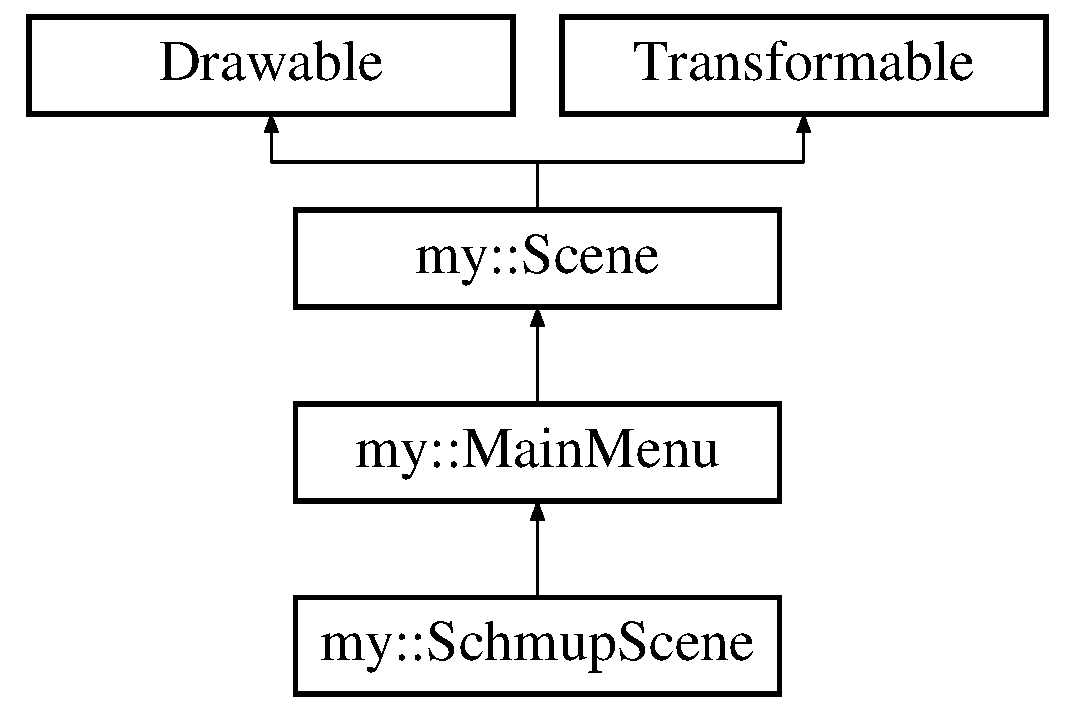
\includegraphics[height=4.000000cm]{classmy_1_1Scene}
\end{center}
\end{figure}
\subsection*{Types publics}
\begin{DoxyCompactItemize}
\item 
\mbox{\Hypertarget{classmy_1_1Scene_a6ad82b3ef155e510d2e0efad7f493f64}\label{classmy_1_1Scene_a6ad82b3ef155e510d2e0efad7f493f64}} 
typedef std\+::shared\+\_\+ptr$<$ \hyperlink{classmy_1_1Scene}{Scene} $>$ {\bfseries Scene\+Ptr}
\end{DoxyCompactItemize}
\subsection*{Fonctions membres publiques}
\begin{DoxyCompactItemize}
\item 
virtual const \hyperlink{structmy_1_1SceneReturnValue}{Scene\+Return\+Value} \hyperlink{classmy_1_1Scene_ae9799de62a6daa9650e040f9f17c78df}{Update} (sf\+::\+Render\+Window \&window)=0  throw (std\+::exception)
\begin{DoxyCompactList}\small\item\em Met à jour les différentes entités. \end{DoxyCompactList}\item 
virtual void \hyperlink{classmy_1_1Scene_ac9401c5ec0e8a740fa338324a7df67a6}{Initialize} (X\+M\+L\+Node\+::\+X\+M\+L\+Node\+Ptr scene\+Root)=0  throw (std\+::out\+\_\+of\+\_\+range, std\+::invalid\+\_\+argument)
\begin{DoxyCompactList}\small\item\em Initialise les entités. \end{DoxyCompactList}\item 
\mbox{\Hypertarget{classmy_1_1Scene_a0077c85b889247ef70d5b4b595bbfa76}\label{classmy_1_1Scene_a0077c85b889247ef70d5b4b595bbfa76}} 
virtual void \hyperlink{classmy_1_1Scene_a0077c85b889247ef70d5b4b595bbfa76}{Reset} ()=0  throw (std\+::out\+\_\+of\+\_\+range, std\+::invalid\+\_\+argument)
\begin{DoxyCompactList}\small\item\em Replace les entités à leurs valeur de base. \end{DoxyCompactList}\end{DoxyCompactItemize}
\subsection*{Fonctions membres protégées}
\begin{DoxyCompactItemize}
\item 
\mbox{\Hypertarget{classmy_1_1Scene_a1e3c785189d466d509f864e70303cbe1}\label{classmy_1_1Scene_a1e3c785189d466d509f864e70303cbe1}} 
virtual void \hyperlink{classmy_1_1Scene_a1e3c785189d466d509f864e70303cbe1}{draw} (sf\+::\+Render\+Target \&target, sf\+::\+Render\+States states) const =0
\begin{DoxyCompactList}\small\item\em Dessine les entités. \end{DoxyCompactList}\item 
void \hyperlink{classmy_1_1Scene_a8e291c764cc4ca5c86c7ff803a7c40c8}{Poll\+Events} (sf\+::\+Render\+Window \&window) noexcept
\begin{DoxyCompactList}\small\item\em Vide la liste des évenements puis récupère les nouveaux évenements de la fenêtre. \end{DoxyCompactList}\end{DoxyCompactItemize}
\subsection*{Attributs protégés}
\begin{DoxyCompactItemize}
\item 
\mbox{\Hypertarget{classmy_1_1Scene_a9f30fe8f2e3a54a0ae79bd5b34a13469}\label{classmy_1_1Scene_a9f30fe8f2e3a54a0ae79bd5b34a13469}} 
std\+::vector$<$ sf\+::\+Event $>$ \hyperlink{classmy_1_1Scene_a9f30fe8f2e3a54a0ae79bd5b34a13469}{m\+\_\+events}
\begin{DoxyCompactList}\small\item\em Tableau d\textquotesingle{}évenements. \end{DoxyCompactList}\end{DoxyCompactItemize}


\subsection{Description détaillée}
Contient des entités dessinable, les mets à jour et peut les dessiner. 

\subsection{Documentation des fonctions membres}
\mbox{\Hypertarget{classmy_1_1Scene_ac9401c5ec0e8a740fa338324a7df67a6}\label{classmy_1_1Scene_ac9401c5ec0e8a740fa338324a7df67a6}} 
\index{my\+::\+Scene@{my\+::\+Scene}!Initialize@{Initialize}}
\index{Initialize@{Initialize}!my\+::\+Scene@{my\+::\+Scene}}
\subsubsection{\texorpdfstring{Initialize()}{Initialize()}}
{\footnotesize\ttfamily virtual void my\+::\+Scene\+::\+Initialize (\begin{DoxyParamCaption}\item[{X\+M\+L\+Node\+::\+X\+M\+L\+Node\+Ptr}]{scene\+Root }\end{DoxyParamCaption}) throw  std\+::out\+\_\+of\+\_\+range, std\+::invalid\+\_\+argument) \hspace{0.3cm}{\ttfamily [pure virtual]}}



Initialise les entités. 

{\bfseries Arguments}~\newline
 scene\+Root\+: Noeud X\+ML contenant les informations sur la scène 

Implémenté dans \hyperlink{classmy_1_1MainMenu_a56e81061a8d8d9a0da77267bd38ec058}{my\+::\+Main\+Menu}, et \hyperlink{classmy_1_1SchmupScene_ad1febbc7aaf1fc8b2eb4d02cdbf3f57a}{my\+::\+Schmup\+Scene}.

\mbox{\Hypertarget{classmy_1_1Scene_a8e291c764cc4ca5c86c7ff803a7c40c8}\label{classmy_1_1Scene_a8e291c764cc4ca5c86c7ff803a7c40c8}} 
\index{my\+::\+Scene@{my\+::\+Scene}!Poll\+Events@{Poll\+Events}}
\index{Poll\+Events@{Poll\+Events}!my\+::\+Scene@{my\+::\+Scene}}
\subsubsection{\texorpdfstring{Poll\+Events()}{PollEvents()}}
{\footnotesize\ttfamily void my\+::\+Scene\+::\+Poll\+Events (\begin{DoxyParamCaption}\item[{sf\+::\+Render\+Window \&}]{window }\end{DoxyParamCaption})\hspace{0.3cm}{\ttfamily [protected]}, {\ttfamily [noexcept]}}



Vide la liste des évenements puis récupère les nouveaux évenements de la fenêtre. 

{\bfseries Arguments}~\newline
 window\+: La fenêtre de rendu actuellement utilisé \mbox{\Hypertarget{classmy_1_1Scene_ae9799de62a6daa9650e040f9f17c78df}\label{classmy_1_1Scene_ae9799de62a6daa9650e040f9f17c78df}} 
\index{my\+::\+Scene@{my\+::\+Scene}!Update@{Update}}
\index{Update@{Update}!my\+::\+Scene@{my\+::\+Scene}}
\subsubsection{\texorpdfstring{Update()}{Update()}}
{\footnotesize\ttfamily virtual const \hyperlink{structmy_1_1SceneReturnValue}{Scene\+Return\+Value} my\+::\+Scene\+::\+Update (\begin{DoxyParamCaption}\item[{sf\+::\+Render\+Window \&}]{window }\end{DoxyParamCaption}) throw  std\+::exception) \hspace{0.3cm}{\ttfamily [pure virtual]}}



Met à jour les différentes entités. 

{\bfseries Arguments}~\newline
 window\+: La fenêtre de rendu actuellement utilisé. 

Implémenté dans \hyperlink{classmy_1_1MainMenu_ada39ad2f51014f08e4526056967daf47}{my\+::\+Main\+Menu}, et \hyperlink{classmy_1_1SchmupScene_ad07d5b2302f0a4250150d51fdcfa1c0b}{my\+::\+Schmup\+Scene}.



La documentation de cette classe a été générée à partir des fichiers suivants \+:\begin{DoxyCompactItemize}
\item 
includes/my\+\_\+graph\+\_\+lib/Scene.\+hpp\item 
lib/my\+\_\+graph\+\_\+lib/Scene.\+cpp\end{DoxyCompactItemize}

\hypertarget{structmy_1_1SceneReturnValue}{}\section{Référence de la structure my\+:\+:Scene\+Return\+Value}
\label{structmy_1_1SceneReturnValue}\index{my\+::\+Scene\+Return\+Value@{my\+::\+Scene\+Return\+Value}}
\subsection*{Fonctions membres publiques}
\begin{DoxyCompactItemize}
\item 
\mbox{\Hypertarget{structmy_1_1SceneReturnValue_a0dac555f3304ef33b0839692ec59cd2d}\label{structmy_1_1SceneReturnValue_a0dac555f3304ef33b0839692ec59cd2d}} 
{\bfseries Scene\+Return\+Value} (S\+T\+A\+T\+E\+\_\+\+R\+E\+T\+U\+RN v=N\+O\+T\+H\+I\+NG, int si=-\/1, bool dr=false, bool di=false)
\end{DoxyCompactItemize}
\subsection*{Attributs publics}
\begin{DoxyCompactItemize}
\item 
\mbox{\Hypertarget{structmy_1_1SceneReturnValue_af7b6ef22567ba94a7126cdf81039441f}\label{structmy_1_1SceneReturnValue_af7b6ef22567ba94a7126cdf81039441f}} 
S\+T\+A\+T\+E\+\_\+\+R\+E\+T\+U\+RN {\bfseries value}
\item 
\mbox{\Hypertarget{structmy_1_1SceneReturnValue_a1b84c148614e916787461194da79c37c}\label{structmy_1_1SceneReturnValue_a1b84c148614e916787461194da79c37c}} 
int {\bfseries new\+Scene\+Index}
\item 
\mbox{\Hypertarget{structmy_1_1SceneReturnValue_a28718d25ad9b2bd6689b8d42cbc743eb}\label{structmy_1_1SceneReturnValue_a28718d25ad9b2bd6689b8d42cbc743eb}} 
bool {\bfseries do\+Reset}
\item 
\mbox{\Hypertarget{structmy_1_1SceneReturnValue_a9cdd936ae735a41f93506da4a6a823aa}\label{structmy_1_1SceneReturnValue_a9cdd936ae735a41f93506da4a6a823aa}} 
bool {\bfseries do\+Initialize}
\end{DoxyCompactItemize}


La documentation de cette structure a été générée à partir du fichier suivant \+:\begin{DoxyCompactItemize}
\item 
includes/my\+\_\+graph\+\_\+lib/Scene\+Return\+Value.\+hh\end{DoxyCompactItemize}

\hypertarget{classmy_1_1SchmupScene}{}\section{Référence de la classe my\+:\+:Schmup\+Scene}
\label{classmy_1_1SchmupScene}\index{my\+::\+Schmup\+Scene@{my\+::\+Schmup\+Scene}}
Graphe d\textquotesingle{}héritage de my\+:\+:Schmup\+Scene\+:\begin{figure}[H]
\begin{center}
\leavevmode
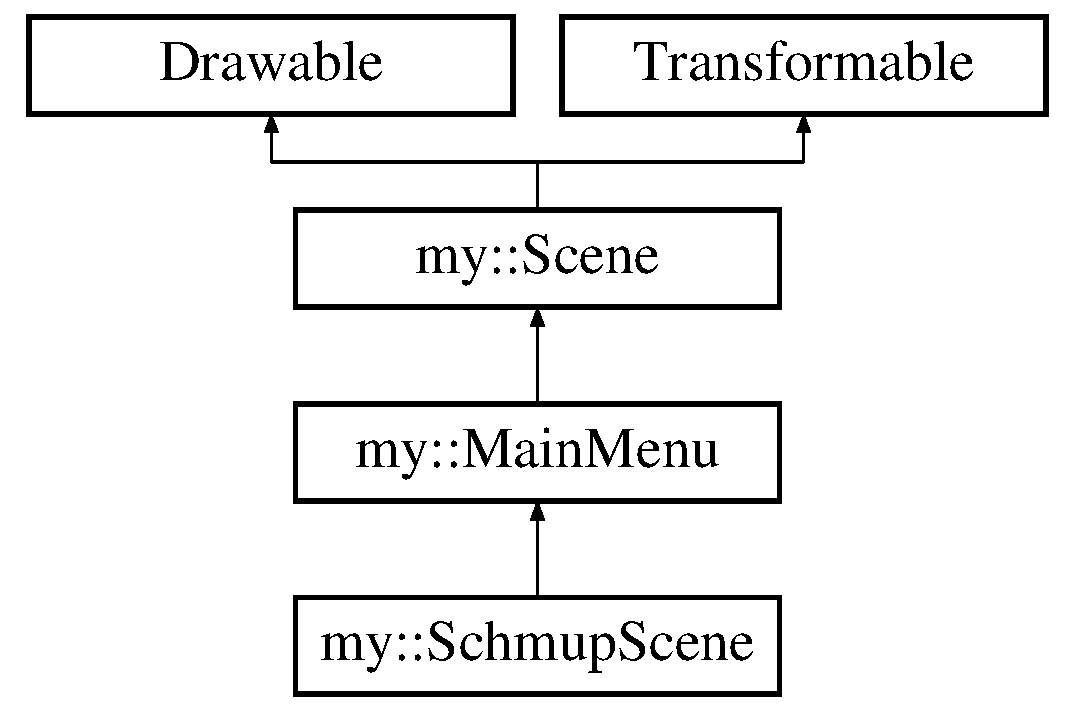
\includegraphics[height=4.000000cm]{classmy_1_1SchmupScene}
\end{center}
\end{figure}
\subsection*{Fonctions membres publiques}
\begin{DoxyCompactItemize}
\item 
virtual const \hyperlink{structmy_1_1SceneReturnValue}{Scene\+Return\+Value} \hyperlink{classmy_1_1SchmupScene_ad07d5b2302f0a4250150d51fdcfa1c0b}{Update} (sf\+::\+Render\+Window \&window)  throw (std\+::exception)
\begin{DoxyCompactList}\small\item\em Met à jour les différentes entités. \end{DoxyCompactList}\item 
virtual void \hyperlink{classmy_1_1SchmupScene_ad1febbc7aaf1fc8b2eb4d02cdbf3f57a}{Initialize} (X\+M\+L\+Node\+::\+X\+M\+L\+Node\+Ptr scene\+Root)  throw (std\+::out\+\_\+of\+\_\+range, std\+::invalid\+\_\+argument)
\begin{DoxyCompactList}\small\item\em Initialise les entités. \end{DoxyCompactList}\item 
\mbox{\Hypertarget{classmy_1_1SchmupScene_afe90a166e047830a86a0e7b331085d20}\label{classmy_1_1SchmupScene_afe90a166e047830a86a0e7b331085d20}} 
virtual void \hyperlink{classmy_1_1SchmupScene_afe90a166e047830a86a0e7b331085d20}{Reset} ()  throw (std\+::out\+\_\+of\+\_\+range, std\+::invalid\+\_\+argument)
\begin{DoxyCompactList}\small\item\em Replace les entités à leurs valeur de base. \end{DoxyCompactList}\end{DoxyCompactItemize}
\subsection*{Fonctions membres protégées}
\begin{DoxyCompactItemize}
\item 
\mbox{\Hypertarget{classmy_1_1SchmupScene_a506ec8d149745caa50d29a69963c892a}\label{classmy_1_1SchmupScene_a506ec8d149745caa50d29a69963c892a}} 
void {\bfseries Initialize\+Player} (X\+M\+L\+Node\+::\+X\+M\+L\+Node\+Ptr player\+Node)  throw (std\+::out\+\_\+of\+\_\+range, std\+::invalid\+\_\+argument)
\item 
\mbox{\Hypertarget{classmy_1_1SchmupScene_af9c2339497a16ad8b47a4f9086e16573}\label{classmy_1_1SchmupScene_af9c2339497a16ad8b47a4f9086e16573}} 
void {\bfseries Initialize\+Enemies\+Pool\+Stage} (X\+M\+L\+Node\+::\+X\+M\+L\+Node\+Ptr stages\+Node)  throw (std\+::out\+\_\+of\+\_\+range, std\+::invalid\+\_\+argument)
\item 
\mbox{\Hypertarget{classmy_1_1SchmupScene_af3913677abc7eb40ecac75765b6f56dd}\label{classmy_1_1SchmupScene_af3913677abc7eb40ecac75765b6f56dd}} 
void {\bfseries Initialize\+Enemies\+Pool\+Enemies} (X\+M\+L\+Node\+::\+X\+M\+L\+Node\+Ptr enemies\+Node)  throw (std\+::out\+\_\+of\+\_\+range, std\+::invalid\+\_\+argument)
\item 
\mbox{\Hypertarget{classmy_1_1SchmupScene_aead67edbc6f62a0855874d78dc379b33}\label{classmy_1_1SchmupScene_aead67edbc6f62a0855874d78dc379b33}} 
void {\bfseries Update\+Player} ()  throw (std\+::out\+\_\+of\+\_\+range)
\item 
\mbox{\Hypertarget{classmy_1_1SchmupScene_a85908a630a1592f2e205254df3711773}\label{classmy_1_1SchmupScene_a85908a630a1592f2e205254df3711773}} 
void {\bfseries Update\+Enemies\+Pool} ()  throw (std\+::out\+\_\+of\+\_\+range)
\item 
\mbox{\Hypertarget{classmy_1_1SchmupScene_a8cfeaa0a042e5fc31eb7ee1618c7304e}\label{classmy_1_1SchmupScene_a8cfeaa0a042e5fc31eb7ee1618c7304e}} 
void {\bfseries Update\+Enemies} ()  throw (std\+::out\+\_\+of\+\_\+range)
\item 
\mbox{\Hypertarget{classmy_1_1SchmupScene_ab2e4aa8b57aa1acc89b8288bbdaf09c0}\label{classmy_1_1SchmupScene_ab2e4aa8b57aa1acc89b8288bbdaf09c0}} 
void {\bfseries Update\+Shoots} ()  throw (std\+::out\+\_\+of\+\_\+range)
\item 
\mbox{\Hypertarget{classmy_1_1SchmupScene_a209f82608e696aa84bc1e97b37d75f20}\label{classmy_1_1SchmupScene_a209f82608e696aa84bc1e97b37d75f20}} 
void {\bfseries Update\+Colisions} ()  throw (std\+::out\+\_\+of\+\_\+range)
\item 
\mbox{\Hypertarget{classmy_1_1SchmupScene_a8f58d7114f5fff2a90b0cc9651745a14}\label{classmy_1_1SchmupScene_a8f58d7114f5fff2a90b0cc9651745a14}} 
void {\bfseries Update\+Objects} ()  throw (std\+::out\+\_\+of\+\_\+range)
\item 
\mbox{\Hypertarget{classmy_1_1SchmupScene_ac31669b2ef8cded3274eb06338812b11}\label{classmy_1_1SchmupScene_ac31669b2ef8cded3274eb06338812b11}} 
virtual void \hyperlink{classmy_1_1SchmupScene_ac31669b2ef8cded3274eb06338812b11}{draw} (sf\+::\+Render\+Target \&target, sf\+::\+Render\+States states) const noexcept
\begin{DoxyCompactList}\small\item\em Dessine les entités. \end{DoxyCompactList}\end{DoxyCompactItemize}
\subsection*{Attributs protégés}
\begin{DoxyCompactItemize}
\item 
\mbox{\Hypertarget{classmy_1_1SchmupScene_adedead0f7c32ba30570d36e9d99fa6dd}\label{classmy_1_1SchmupScene_adedead0f7c32ba30570d36e9d99fa6dd}} 
\hyperlink{classmy_1_1EnemiesPool}{Enemies\+Pool} {\bfseries m\+\_\+enemies\+Pool}
\item 
\mbox{\Hypertarget{classmy_1_1SchmupScene_a322c62de636efb2272f75530b9f28abc}\label{classmy_1_1SchmupScene_a322c62de636efb2272f75530b9f28abc}} 
Player\+::\+Player\+Ptr {\bfseries m\+\_\+player}
\item 
\mbox{\Hypertarget{classmy_1_1SchmupScene_a4eafc8d5a8d22545911e3155ce8bdbd1}\label{classmy_1_1SchmupScene_a4eafc8d5a8d22545911e3155ce8bdbd1}} 
Enemies\+Pool\+::\+Enemies\+List {\bfseries m\+\_\+enemies}
\item 
\mbox{\Hypertarget{classmy_1_1SchmupScene_ad9f91bea3c07dbca83fa978aeaa711f0}\label{classmy_1_1SchmupScene_ad9f91bea3c07dbca83fa978aeaa711f0}} 
Shooter\+::\+Shoot\+List {\bfseries m\+\_\+player\+Shoots}
\item 
\mbox{\Hypertarget{classmy_1_1SchmupScene_a7bfa7fdac07f775b59d6f88eb784d0e2}\label{classmy_1_1SchmupScene_a7bfa7fdac07f775b59d6f88eb784d0e2}} 
Shooter\+::\+Shoot\+List {\bfseries m\+\_\+enemies\+Shoots}
\end{DoxyCompactItemize}
\subsection*{Attributs protégés statiques}
\begin{DoxyCompactItemize}
\item 
\mbox{\Hypertarget{classmy_1_1SchmupScene_a40d188c2857e5d7ca60db7b4fc398060}\label{classmy_1_1SchmupScene_a40d188c2857e5d7ca60db7b4fc398060}} 
static const std\+::string {\bfseries S\+C\+E\+N\+E\+\_\+\+P\+L\+A\+Y\+E\+R\+\_\+\+N\+O\+DE} = \char`\"{}player\char`\"{}
\item 
\mbox{\Hypertarget{classmy_1_1SchmupScene_a2d33751f6a799a8a18d4bdeeb94a8fbf}\label{classmy_1_1SchmupScene_a2d33751f6a799a8a18d4bdeeb94a8fbf}} 
static const std\+::string {\bfseries S\+C\+E\+N\+E\+\_\+\+S\+T\+A\+G\+E\+S\+\_\+\+N\+O\+DE} = \char`\"{}stages\char`\"{}
\item 
\mbox{\Hypertarget{classmy_1_1SchmupScene_af4c45e8c47507287ef6e8cf1b147beca}\label{classmy_1_1SchmupScene_af4c45e8c47507287ef6e8cf1b147beca}} 
static const std\+::string {\bfseries S\+C\+E\+N\+E\+\_\+\+E\+N\+E\+M\+I\+E\+S\+\_\+\+N\+O\+DE} = \char`\"{}enemies\char`\"{}
\end{DoxyCompactItemize}
\subsection*{Membres hérités additionnels}


\subsection{Documentation des fonctions membres}
\mbox{\Hypertarget{classmy_1_1SchmupScene_ad1febbc7aaf1fc8b2eb4d02cdbf3f57a}\label{classmy_1_1SchmupScene_ad1febbc7aaf1fc8b2eb4d02cdbf3f57a}} 
\index{my\+::\+Schmup\+Scene@{my\+::\+Schmup\+Scene}!Initialize@{Initialize}}
\index{Initialize@{Initialize}!my\+::\+Schmup\+Scene@{my\+::\+Schmup\+Scene}}
\subsubsection{\texorpdfstring{Initialize()}{Initialize()}}
{\footnotesize\ttfamily void my\+::\+Schmup\+Scene\+::\+Initialize (\begin{DoxyParamCaption}\item[{X\+M\+L\+Node\+::\+X\+M\+L\+Node\+Ptr}]{scene\+Root }\end{DoxyParamCaption}) throw  std\+::out\+\_\+of\+\_\+range, std\+::invalid\+\_\+argument) \hspace{0.3cm}{\ttfamily [virtual]}}



Initialise les entités. 

{\bfseries Arguments}~\newline
 scene\+Root\+: Noeud X\+ML contenant les informations sur la scène 

Réimplémentée à partir de \hyperlink{classmy_1_1MainMenu_a56e81061a8d8d9a0da77267bd38ec058}{my\+::\+Main\+Menu}.

\mbox{\Hypertarget{classmy_1_1SchmupScene_ad07d5b2302f0a4250150d51fdcfa1c0b}\label{classmy_1_1SchmupScene_ad07d5b2302f0a4250150d51fdcfa1c0b}} 
\index{my\+::\+Schmup\+Scene@{my\+::\+Schmup\+Scene}!Update@{Update}}
\index{Update@{Update}!my\+::\+Schmup\+Scene@{my\+::\+Schmup\+Scene}}
\subsubsection{\texorpdfstring{Update()}{Update()}}
{\footnotesize\ttfamily const \hyperlink{structmy_1_1SceneReturnValue}{my\+::\+Scene\+Return\+Value} my\+::\+Schmup\+Scene\+::\+Update (\begin{DoxyParamCaption}\item[{sf\+::\+Render\+Window \&}]{window }\end{DoxyParamCaption}) throw  std\+::exception) \hspace{0.3cm}{\ttfamily [virtual]}}



Met à jour les différentes entités. 

{\bfseries Arguments}~\newline
 window\+: La fenêtre de rendu actuellement utilisé. 

Réimplémentée à partir de \hyperlink{classmy_1_1MainMenu_ada39ad2f51014f08e4526056967daf47}{my\+::\+Main\+Menu}.



La documentation de cette classe a été générée à partir des fichiers suivants \+:\begin{DoxyCompactItemize}
\item 
includes/my\+\_\+menu\+\_\+lib/Schmup\+Scene.\+hpp\item 
lib/my\+\_\+menu\+\_\+lib/Schmup\+Scene.\+cpp\end{DoxyCompactItemize}

\hypertarget{classmy_1_1Shooter}{}\section{Référence de la classe my\+:\+:Shooter}
\label{classmy_1_1Shooter}\index{my\+::\+Shooter@{my\+::\+Shooter}}
Graphe d\textquotesingle{}héritage de my\+:\+:Shooter\+:\begin{figure}[H]
\begin{center}
\leavevmode
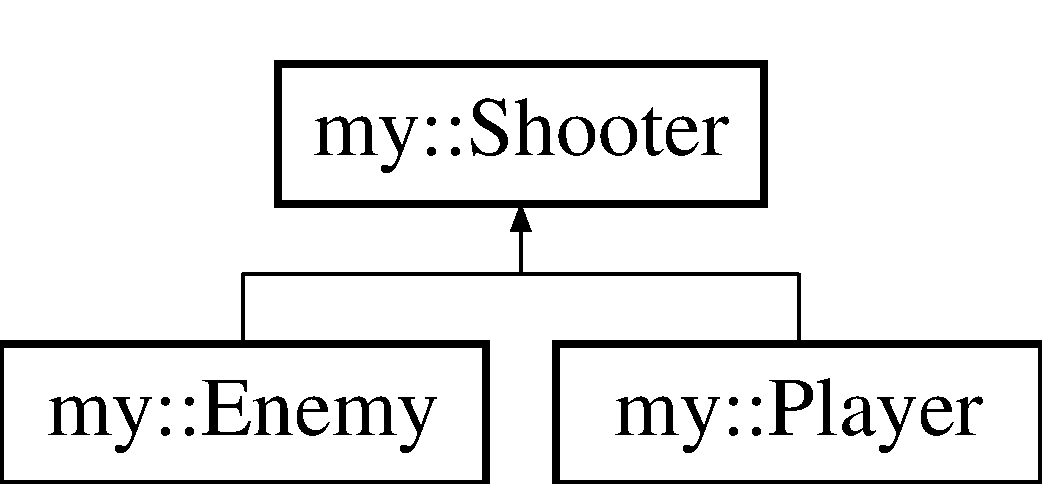
\includegraphics[height=2.000000cm]{classmy_1_1Shooter}
\end{center}
\end{figure}
\subsection*{Types publics}
\begin{DoxyCompactItemize}
\item 
\mbox{\Hypertarget{classmy_1_1Shooter_a82aae5a56bed644b983bfb3f926950d2}\label{classmy_1_1Shooter_a82aae5a56bed644b983bfb3f926950d2}} 
typedef std\+::shared\+\_\+ptr$<$ \hyperlink{classmy_1_1Shooter}{Shooter} $>$ {\bfseries Shooter\+Ptr}
\item 
\mbox{\Hypertarget{classmy_1_1Shooter_adc320a69e79962464e86f701d2b728d1}\label{classmy_1_1Shooter_adc320a69e79962464e86f701d2b728d1}} 
typedef std\+::vector$<$ Bullet\+::\+Bullet\+Ptr $>$ {\bfseries Shoot\+List}
\item 
\mbox{\Hypertarget{classmy_1_1Shooter_ad2fe17c54adc480568a891fb04ce8242}\label{classmy_1_1Shooter_ad2fe17c54adc480568a891fb04ce8242}} 
typedef std\+::map$<$ const std\+::string, X\+M\+L\+Node\+::\+X\+M\+L\+Node\+Ptr $>$ {\bfseries Shoot\+Nodes}
\end{DoxyCompactItemize}
\subsection*{Fonctions membres publiques}
\begin{DoxyCompactItemize}
\item 
\mbox{\Hypertarget{classmy_1_1Shooter_a074f3f97399ae7f4b93d365cda93610c}\label{classmy_1_1Shooter_a074f3f97399ae7f4b93d365cda93610c}} 
bool {\bfseries Can\+Shoot} () const noexcept
\item 
\mbox{\Hypertarget{classmy_1_1Shooter_a829b2be6f57ce7d21ade456380168d86}\label{classmy_1_1Shooter_a829b2be6f57ce7d21ade456380168d86}} 
const Shoot\+List {\bfseries Get\+Shoot\+List} () const  throw (std\+::out\+\_\+of\+\_\+range, std\+::invalid\+\_\+argument)
\item 
\mbox{\Hypertarget{classmy_1_1Shooter_a8bd2cf898da70f9ab05e1b3d9a8f246f}\label{classmy_1_1Shooter_a8bd2cf898da70f9ab05e1b3d9a8f246f}} 
const Shoot\+Nodes \& {\bfseries Get\+Shoot\+Nodes} () const noexcept
\item 
\mbox{\Hypertarget{classmy_1_1Shooter_aaeab68a3e46942098d351b7958afa04e}\label{classmy_1_1Shooter_aaeab68a3e46942098d351b7958afa04e}} 
const std\+::string \& {\bfseries Get\+Shoot\+Key} () const noexcept
\item 
\mbox{\Hypertarget{classmy_1_1Shooter_ab8882679b9b128e2b0f9b036b584ac58}\label{classmy_1_1Shooter_ab8882679b9b128e2b0f9b036b584ac58}} 
const unsigned {\bfseries Get\+Shoot\+Framerate\+Max} () const noexcept
\item 
\mbox{\Hypertarget{classmy_1_1Shooter_a5e8b4144be7d18ecd74cefff1d1ec696}\label{classmy_1_1Shooter_a5e8b4144be7d18ecd74cefff1d1ec696}} 
void {\bfseries Set\+Can\+Shoot} (bool can\+Shoot) noexcept
\item 
\mbox{\Hypertarget{classmy_1_1Shooter_a2f99b7f7802dd20fec49e571cfcfb887}\label{classmy_1_1Shooter_a2f99b7f7802dd20fec49e571cfcfb887}} 
void {\bfseries Set\+Shoot\+Nodes} (const Shoot\+Nodes \&shoot\+Nodes) noexcept
\item 
\mbox{\Hypertarget{classmy_1_1Shooter_a2b6302544a8010b4f379c353ed6bfbac}\label{classmy_1_1Shooter_a2b6302544a8010b4f379c353ed6bfbac}} 
void {\bfseries Add\+Shoot\+Node} (const std\+::string \&str, X\+M\+L\+Node\+::\+X\+M\+L\+Node\+Ptr new\+Shoot\+Node)  throw (std\+::invalid\+\_\+argument)
\item 
\mbox{\Hypertarget{classmy_1_1Shooter_afe3aa39abd0c4131b811596dcffa45a6}\label{classmy_1_1Shooter_afe3aa39abd0c4131b811596dcffa45a6}} 
void {\bfseries Set\+Shoot\+Key} (const std\+::string \&key) noexcept
\item 
\mbox{\Hypertarget{classmy_1_1Shooter_ada55bbd697ad01242a5cbb07b691b27d}\label{classmy_1_1Shooter_ada55bbd697ad01242a5cbb07b691b27d}} 
void {\bfseries Set\+Shoot\+Framerate\+Max} (unsigned shoot\+Framerate\+Max) noexcept
\end{DoxyCompactItemize}
\subsection*{Fonctions membres protégées}
\begin{DoxyCompactItemize}
\item 
\mbox{\Hypertarget{classmy_1_1Shooter_a0e5a30cdfabf48052d2484c2e2ca6f6f}\label{classmy_1_1Shooter_a0e5a30cdfabf48052d2484c2e2ca6f6f}} 
void {\bfseries Update} () noexcept
\end{DoxyCompactItemize}
\subsection*{Attributs protégés}
\begin{DoxyCompactItemize}
\item 
\mbox{\Hypertarget{classmy_1_1Shooter_a829743ae534a86061d3359aa4466109c}\label{classmy_1_1Shooter_a829743ae534a86061d3359aa4466109c}} 
bool {\bfseries m\+\_\+can\+Shoot}
\item 
\mbox{\Hypertarget{classmy_1_1Shooter_a7f28784709dcee6b6379a96ed02af6cc}\label{classmy_1_1Shooter_a7f28784709dcee6b6379a96ed02af6cc}} 
Shoot\+Nodes {\bfseries m\+\_\+shoot\+Nodes}
\item 
\mbox{\Hypertarget{classmy_1_1Shooter_a772980b6cb2304b5b7f58b538f97ff0b}\label{classmy_1_1Shooter_a772980b6cb2304b5b7f58b538f97ff0b}} 
std\+::string {\bfseries m\+\_\+shoot\+Key}
\item 
\mbox{\Hypertarget{classmy_1_1Shooter_abecd4ad91ecd7c2ae5a3f629078f4969}\label{classmy_1_1Shooter_abecd4ad91ecd7c2ae5a3f629078f4969}} 
unsigned {\bfseries m\+\_\+shoot\+Framerate\+Max}
\end{DoxyCompactItemize}


La documentation de cette classe a été générée à partir des fichiers suivants \+:\begin{DoxyCompactItemize}
\item 
includes/my\+\_\+objects\+\_\+lib/Shooter.\+hpp\item 
lib/my\+\_\+objects\+\_\+lib/Shooter.\+cpp\end{DoxyCompactItemize}

\hypertarget{classmy_1_1SpriteButton}{}\section{Référence de la classe my\+:\+:Sprite\+Button}
\label{classmy_1_1SpriteButton}\index{my\+::\+Sprite\+Button@{my\+::\+Sprite\+Button}}
Graphe d\textquotesingle{}héritage de my\+:\+:Sprite\+Button\+:\begin{figure}[H]
\begin{center}
\leavevmode
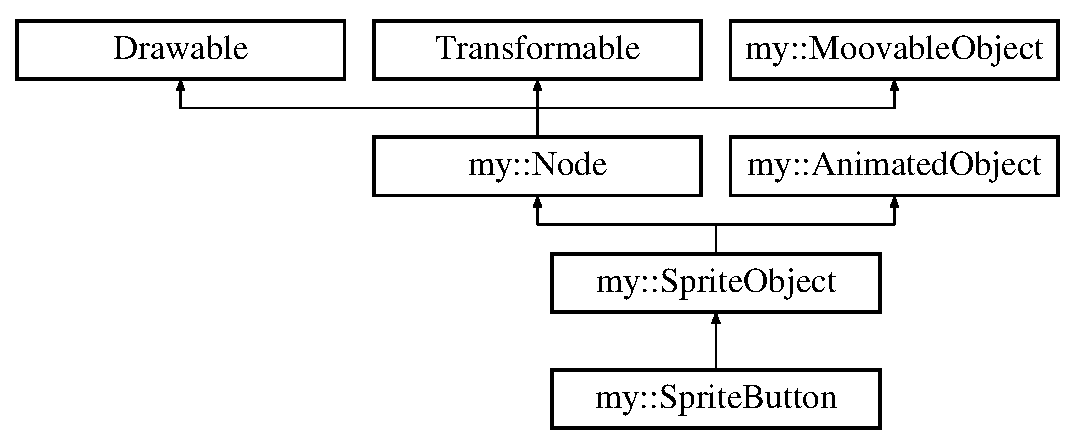
\includegraphics[height=4.000000cm]{classmy_1_1SpriteButton}
\end{center}
\end{figure}
\subsection*{Types publics}
\begin{DoxyCompactItemize}
\item 
\mbox{\Hypertarget{classmy_1_1SpriteButton_ac168ec0a97a3c5ea31154e654157393b}\label{classmy_1_1SpriteButton_ac168ec0a97a3c5ea31154e654157393b}} 
typedef std\+::shared\+\_\+ptr$<$ \hyperlink{classmy_1_1SpriteButton}{Sprite\+Button} $>$ {\bfseries Sprite\+Button\+Ptr}
\end{DoxyCompactItemize}
\subsection*{Fonctions membres publiques}
\begin{DoxyCompactItemize}
\item 
\mbox{\Hypertarget{classmy_1_1SpriteButton_a84f4ff8cdb411c3e9d555eacd390f19c}\label{classmy_1_1SpriteButton_a84f4ff8cdb411c3e9d555eacd390f19c}} 
virtual void {\bfseries Update} (const sf\+::\+Vector2f \&mouse\+Pos)  throw (std\+::out\+\_\+of\+\_\+range)
\end{DoxyCompactItemize}
\subsection*{Fonctions membres protégées}
\begin{DoxyCompactItemize}
\item 
\mbox{\Hypertarget{classmy_1_1SpriteButton_ae2f9b647749c3380a38fff6341117a1a}\label{classmy_1_1SpriteButton_ae2f9b647749c3380a38fff6341117a1a}} 
virtual void {\bfseries Update} ()  throw (std\+::out\+\_\+of\+\_\+range)
\item 
\mbox{\Hypertarget{classmy_1_1SpriteButton_a997274cd61466d69104e37f274485ab4}\label{classmy_1_1SpriteButton_a997274cd61466d69104e37f274485ab4}} 
virtual void {\bfseries Update\+Mouse} (const sf\+::\+Vector2f \&mouse\+Pos)
\item 
\mbox{\Hypertarget{classmy_1_1SpriteButton_acd9b680033cd93cb7ce3cb01935edc87}\label{classmy_1_1SpriteButton_acd9b680033cd93cb7ce3cb01935edc87}} 
virtual void {\bfseries Update\+Animation} ()  throw (std\+::out\+\_\+of\+\_\+range)
\end{DoxyCompactItemize}
\subsection*{Attributs protégés}
\begin{DoxyCompactItemize}
\item 
\mbox{\Hypertarget{classmy_1_1SpriteButton_a0972a48b66dab6e0949863d177b86f99}\label{classmy_1_1SpriteButton_a0972a48b66dab6e0949863d177b86f99}} 
bool {\bfseries m\+\_\+is\+Mouse\+Overed}
\item 
\mbox{\Hypertarget{classmy_1_1SpriteButton_a56929961aa06e613d74ff2c70ad1f1b5}\label{classmy_1_1SpriteButton_a56929961aa06e613d74ff2c70ad1f1b5}} 
bool {\bfseries m\+\_\+is\+Clicked}
\end{DoxyCompactItemize}
\subsection*{Attributs protégés statiques}
\begin{DoxyCompactItemize}
\item 
\mbox{\Hypertarget{classmy_1_1SpriteButton_a71bf74337f795f1b5755b767c19b164b}\label{classmy_1_1SpriteButton_a71bf74337f795f1b5755b767c19b164b}} 
static const std\+::string {\bfseries O\+N\+\_\+\+C\+L\+I\+C\+K\+\_\+\+A\+N\+I\+M\+\_\+\+N\+A\+ME} = \char`\"{}on\+\_\+click\char`\"{}
\item 
\mbox{\Hypertarget{classmy_1_1SpriteButton_a2a6d4d8c6943d38854dfb59410ef8a7f}\label{classmy_1_1SpriteButton_a2a6d4d8c6943d38854dfb59410ef8a7f}} 
static const std\+::string {\bfseries O\+N\+\_\+\+M\+O\+U\+S\+E\+\_\+\+O\+V\+E\+R\+\_\+\+A\+N\+I\+M\+\_\+\+N\+A\+ME} = \char`\"{}on\+\_\+mouse\+\_\+over\char`\"{}
\end{DoxyCompactItemize}


La documentation de cette classe a été générée à partir des fichiers suivants \+:\begin{DoxyCompactItemize}
\item 
includes/my\+\_\+objects\+\_\+lib/Sprite\+Button.\+hpp\item 
lib/my\+\_\+objects\+\_\+lib/Sprite\+Button.\+cpp\end{DoxyCompactItemize}

\hypertarget{classmy_1_1SpriteObject}{}\section{Référence de la classe my\+:\+:Sprite\+Object}
\label{classmy_1_1SpriteObject}\index{my\+::\+Sprite\+Object@{my\+::\+Sprite\+Object}}
Graphe d\textquotesingle{}héritage de my\+:\+:Sprite\+Object\+:\begin{figure}[H]
\begin{center}
\leavevmode
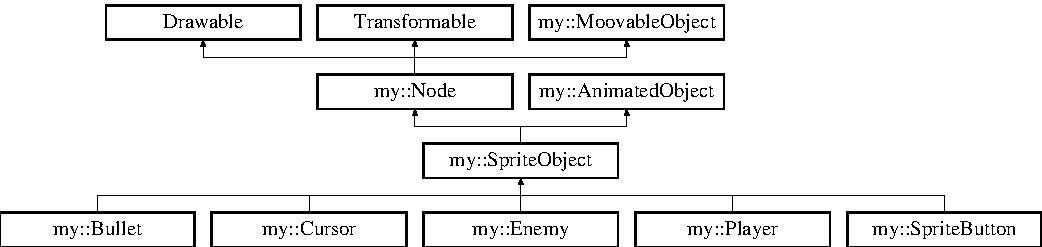
\includegraphics[height=3.318518cm]{classmy_1_1SpriteObject}
\end{center}
\end{figure}
\subsection*{Types publics}
\begin{DoxyCompactItemize}
\item 
\mbox{\Hypertarget{classmy_1_1SpriteObject_a46560ae2f177e36d7025242b5cfd7401}\label{classmy_1_1SpriteObject_a46560ae2f177e36d7025242b5cfd7401}} 
typedef std\+::shared\+\_\+ptr$<$ \hyperlink{classmy_1_1SpriteObject}{Sprite\+Object} $>$ {\bfseries Sprite\+Object\+Ptr}
\end{DoxyCompactItemize}
\subsection*{Fonctions membres publiques}
\begin{DoxyCompactItemize}
\item 
\mbox{\Hypertarget{classmy_1_1SpriteObject_a02631a9375ca3b75fb8e57c2fb678b0c}\label{classmy_1_1SpriteObject_a02631a9375ca3b75fb8e57c2fb678b0c}} 
virtual bool {\bfseries Is\+Intersect} (const sf\+::\+Vector2f \&point) const noexcept
\item 
\mbox{\Hypertarget{classmy_1_1SpriteObject_a1700db880801ebcbb32cf48a0bf011b6}\label{classmy_1_1SpriteObject_a1700db880801ebcbb32cf48a0bf011b6}} 
virtual bool {\bfseries Is\+Intersect} (const sf\+::\+Float\+Rect \&square) const noexcept
\item 
\mbox{\Hypertarget{classmy_1_1SpriteObject_aa41083f207f9ef3e3bcfef14a959c492}\label{classmy_1_1SpriteObject_aa41083f207f9ef3e3bcfef14a959c492}} 
virtual const sf\+::\+Float\+Rect {\bfseries Get\+Hit\+Box} () const noexcept
\item 
\mbox{\Hypertarget{classmy_1_1SpriteObject_a49398fd0213bbbd95f7beb9496df2ecf}\label{classmy_1_1SpriteObject_a49398fd0213bbbd95f7beb9496df2ecf}} 
virtual void {\bfseries Update} ()  throw (std\+::out\+\_\+of\+\_\+range)
\item 
\mbox{\Hypertarget{classmy_1_1SpriteObject_a8f23dad9d0a73b6e48c411c555fee70c}\label{classmy_1_1SpriteObject_a8f23dad9d0a73b6e48c411c555fee70c}} 
void {\bfseries Set\+Texture} (const sf\+::\+Texture \&texture) noexcept
\item 
\mbox{\Hypertarget{classmy_1_1SpriteObject_aaee4594452b0b9e08b65348185aa1855}\label{classmy_1_1SpriteObject_aaee4594452b0b9e08b65348185aa1855}} 
void {\bfseries Set\+Color} (const sf\+::\+Color \&color) noexcept
\item 
\mbox{\Hypertarget{classmy_1_1SpriteObject_addfa5e1323015cf8829e922b8a550e9c}\label{classmy_1_1SpriteObject_addfa5e1323015cf8829e922b8a550e9c}} 
void {\bfseries Set\+Rotate} (float rotate) noexcept
\item 
\mbox{\Hypertarget{classmy_1_1SpriteObject_aaaac0961989244f2826c683d95e9caec}\label{classmy_1_1SpriteObject_aaaac0961989244f2826c683d95e9caec}} 
void {\bfseries Set\+Scale} (float scaleX, float scaleY) noexcept
\item 
\mbox{\Hypertarget{classmy_1_1SpriteObject_ac7b290f44c1430d972ba0045bd888aaf}\label{classmy_1_1SpriteObject_ac7b290f44c1430d972ba0045bd888aaf}} 
void {\bfseries Set\+Scale} (const sf\+::\+Vector2f \&scale) noexcept
\item 
\mbox{\Hypertarget{classmy_1_1SpriteObject_a828bc053284a62494605a76c53498858}\label{classmy_1_1SpriteObject_a828bc053284a62494605a76c53498858}} 
void {\bfseries Set\+Origin} (float origX, float origY) noexcept
\item 
\mbox{\Hypertarget{classmy_1_1SpriteObject_a0b5ce634af99d1651069cdb0c9c10dbe}\label{classmy_1_1SpriteObject_a0b5ce634af99d1651069cdb0c9c10dbe}} 
void {\bfseries Set\+Subrect} (const sf\+::\+Int\+Rect \&subrect) noexcept
\item 
\mbox{\Hypertarget{classmy_1_1SpriteObject_a3ce90b6e8a95d73ba346c2b993a74dec}\label{classmy_1_1SpriteObject_a3ce90b6e8a95d73ba346c2b993a74dec}} 
const sf\+::\+Sprite \& {\bfseries Get\+Sprite} () const noexcept
\end{DoxyCompactItemize}
\subsection*{Fonctions membres protégées}
\begin{DoxyCompactItemize}
\item 
\mbox{\Hypertarget{classmy_1_1SpriteObject_a5ad1c5e9b8ac2b0089f1de5bf616c245}\label{classmy_1_1SpriteObject_a5ad1c5e9b8ac2b0089f1de5bf616c245}} 
virtual void {\bfseries Update\+Animation} ()  throw (std\+::out\+\_\+of\+\_\+range)
\item 
\mbox{\Hypertarget{classmy_1_1SpriteObject_a6dbc79fd834894570763f975c5de7920}\label{classmy_1_1SpriteObject_a6dbc79fd834894570763f975c5de7920}} 
virtual void {\bfseries draw} (sf\+::\+Render\+Target \&target, sf\+::\+Render\+States states) const noexcept
\end{DoxyCompactItemize}
\subsection*{Attributs protégés}
\begin{DoxyCompactItemize}
\item 
\mbox{\Hypertarget{classmy_1_1SpriteObject_aede108105767fe39028727a225a24105}\label{classmy_1_1SpriteObject_aede108105767fe39028727a225a24105}} 
sf\+::\+Sprite {\bfseries m\+\_\+sprite}
\end{DoxyCompactItemize}
\subsection*{Membres hérités additionnels}


La documentation de cette classe a été générée à partir des fichiers suivants \+:\begin{DoxyCompactItemize}
\item 
includes/my\+\_\+graph\+\_\+lib/Sprite\+Object.\+hpp\item 
lib/my\+\_\+graph\+\_\+lib/Sprite\+Object.\+cpp\end{DoxyCompactItemize}

\hypertarget{classmy_1_1TextObject}{}\section{Référence de la classe my\+:\+:Text\+Object}
\label{classmy_1_1TextObject}\index{my\+::\+Text\+Object@{my\+::\+Text\+Object}}
Graphe d\textquotesingle{}héritage de my\+:\+:Text\+Object\+:\begin{figure}[H]
\begin{center}
\leavevmode
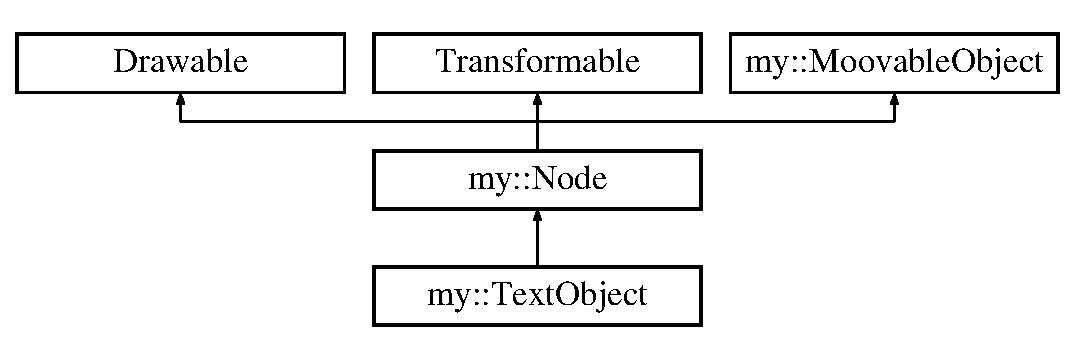
\includegraphics[height=3.000000cm]{classmy_1_1TextObject}
\end{center}
\end{figure}
\subsection*{Types publics}
\begin{DoxyCompactItemize}
\item 
\mbox{\Hypertarget{classmy_1_1TextObject_aea72cf536c84838a0db2be2204db2ba8}\label{classmy_1_1TextObject_aea72cf536c84838a0db2be2204db2ba8}} 
typedef std\+::shared\+\_\+ptr$<$ \hyperlink{classmy_1_1TextObject}{Text\+Object} $>$ {\bfseries Text\+Object\+Ptr}
\end{DoxyCompactItemize}
\subsection*{Fonctions membres publiques}
\begin{DoxyCompactItemize}
\item 
\mbox{\Hypertarget{classmy_1_1TextObject_affb75169f05260a87266c07dde14ee5a}\label{classmy_1_1TextObject_affb75169f05260a87266c07dde14ee5a}} 
virtual bool {\bfseries Is\+Intersect} (const sf\+::\+Vector2f \&point) const noexcept
\item 
\mbox{\Hypertarget{classmy_1_1TextObject_a26eda23e4fec449c8f402cf2521135fd}\label{classmy_1_1TextObject_a26eda23e4fec449c8f402cf2521135fd}} 
virtual bool {\bfseries Is\+Intersect} (const sf\+::\+Float\+Rect \&square) const noexcept
\item 
\mbox{\Hypertarget{classmy_1_1TextObject_aa297b3eab77e5a331eec8c7d641804b3}\label{classmy_1_1TextObject_aa297b3eab77e5a331eec8c7d641804b3}} 
virtual const sf\+::\+Float\+Rect {\bfseries Get\+Hit\+Box} () const noexcept
\item 
\mbox{\Hypertarget{classmy_1_1TextObject_af4e932250fe1ea36d747b552ebd7671b}\label{classmy_1_1TextObject_af4e932250fe1ea36d747b552ebd7671b}} 
void {\bfseries Set\+Font} (const sf\+::\+Font \&font) noexcept
\item 
\mbox{\Hypertarget{classmy_1_1TextObject_a8551ba9793ef0c670549c1bc03158727}\label{classmy_1_1TextObject_a8551ba9793ef0c670549c1bc03158727}} 
void {\bfseries Set\+Text} (const std\+::string \&text) noexcept
\item 
\mbox{\Hypertarget{classmy_1_1TextObject_a7f1bd59113e2d200c3d5384e78d6fcc0}\label{classmy_1_1TextObject_a7f1bd59113e2d200c3d5384e78d6fcc0}} 
void {\bfseries Set\+Size} (int size) noexcept
\item 
\mbox{\Hypertarget{classmy_1_1TextObject_a0e5ecb2bb4069f183fc84d6912a91c87}\label{classmy_1_1TextObject_a0e5ecb2bb4069f183fc84d6912a91c87}} 
void {\bfseries Set\+Color} (const sf\+::\+Color \&color) noexcept
\item 
\mbox{\Hypertarget{classmy_1_1TextObject_a1e5d9ee2e21e5ad6282f559da6ac6097}\label{classmy_1_1TextObject_a1e5d9ee2e21e5ad6282f559da6ac6097}} 
void {\bfseries Set\+Rotate} (float rotate) noexcept
\item 
\mbox{\Hypertarget{classmy_1_1TextObject_a86747805eb38d71b850f620d7ccce3f0}\label{classmy_1_1TextObject_a86747805eb38d71b850f620d7ccce3f0}} 
void {\bfseries Set\+Scale} (float scaleX, float scaleY) noexcept
\item 
\mbox{\Hypertarget{classmy_1_1TextObject_a7c40c8ac5e3d1400dc09f11634986e32}\label{classmy_1_1TextObject_a7c40c8ac5e3d1400dc09f11634986e32}} 
void {\bfseries Set\+Scale} (const sf\+::\+Vector2f \&scale) noexcept
\item 
\mbox{\Hypertarget{classmy_1_1TextObject_a52cbdf029fb1197a4e4820713325e0c7}\label{classmy_1_1TextObject_a52cbdf029fb1197a4e4820713325e0c7}} 
void {\bfseries Set\+Origin} (float origX, float origxY) noexcept
\item 
\mbox{\Hypertarget{classmy_1_1TextObject_aa57b37a35c4b47f52532c36b1de7016b}\label{classmy_1_1TextObject_aa57b37a35c4b47f52532c36b1de7016b}} 
const sf\+::\+Text \& {\bfseries Get\+Text} () const noexcept
\end{DoxyCompactItemize}
\subsection*{Fonctions membres protégées}
\begin{DoxyCompactItemize}
\item 
\mbox{\Hypertarget{classmy_1_1TextObject_aaa3cb42fe369ae9c6f8d1f4e495b3d7b}\label{classmy_1_1TextObject_aaa3cb42fe369ae9c6f8d1f4e495b3d7b}} 
virtual void {\bfseries draw} (sf\+::\+Render\+Target \&target, sf\+::\+Render\+States states) const noexcept
\end{DoxyCompactItemize}
\subsection*{Attributs protégés}
\begin{DoxyCompactItemize}
\item 
\mbox{\Hypertarget{classmy_1_1TextObject_aa00d09e7bbea62c94333d54ef500e11d}\label{classmy_1_1TextObject_aa00d09e7bbea62c94333d54ef500e11d}} 
sf\+::\+Text {\bfseries m\+\_\+text}
\end{DoxyCompactItemize}
\subsection*{Membres hérités additionnels}


La documentation de cette classe a été générée à partir des fichiers suivants \+:\begin{DoxyCompactItemize}
\item 
includes/my\+\_\+graph\+\_\+lib/Text\+Object.\+hpp\item 
lib/my\+\_\+graph\+\_\+lib/Text\+Object.\+cpp\end{DoxyCompactItemize}

\hypertarget{structmy_1_1WindowBuffer}{}\section{Référence de la structure my\+:\+:Window\+Buffer}
\label{structmy_1_1WindowBuffer}\index{my\+::\+Window\+Buffer@{my\+::\+Window\+Buffer}}


Fenêtre de rendu. Contient les différentes scènes du jeu.  




{\ttfamily \#include $<$Window\+Buffer.\+hh$>$}

Graphe d\textquotesingle{}héritage de my\+:\+:Window\+Buffer\+:\begin{figure}[H]
\begin{center}
\leavevmode
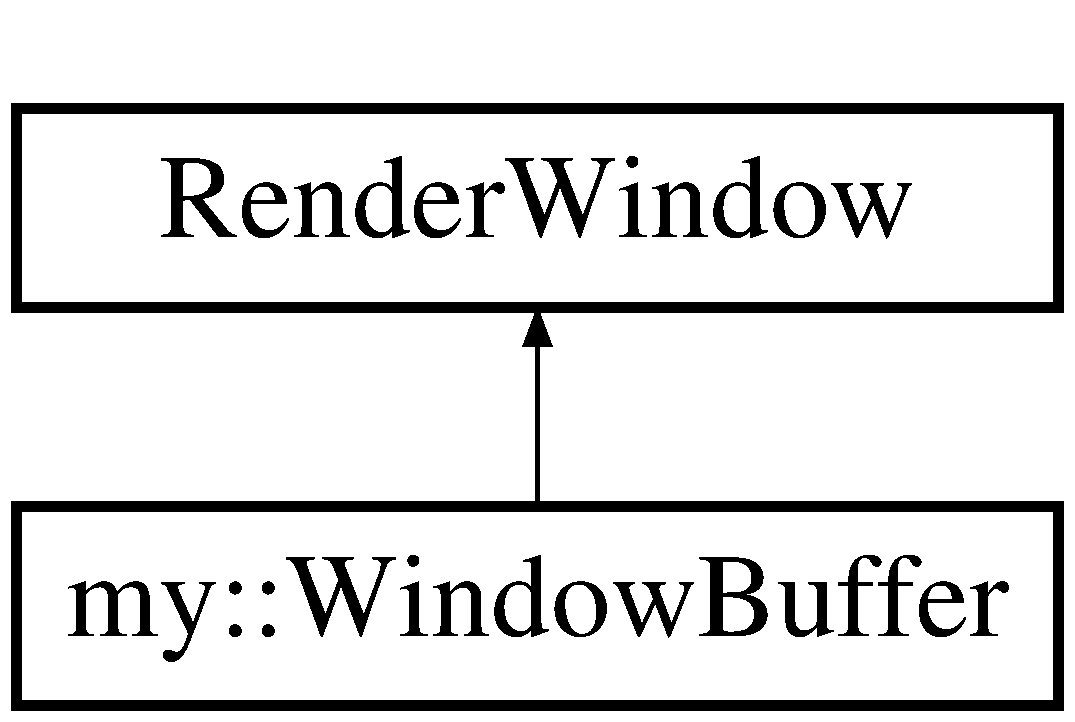
\includegraphics[height=2.000000cm]{structmy_1_1WindowBuffer}
\end{center}
\end{figure}
\subsection*{Types publics}
\begin{DoxyCompactItemize}
\item 
\mbox{\Hypertarget{structmy_1_1WindowBuffer_a1a2f9ba69300d5a3bf64a72384dfd058}\label{structmy_1_1WindowBuffer_a1a2f9ba69300d5a3bf64a72384dfd058}} 
typedef std\+::shared\+\_\+ptr$<$ \hyperlink{structmy_1_1WindowBuffer}{Window\+Buffer} $>$ {\bfseries Window\+Buffer\+Ptr}
\end{DoxyCompactItemize}
\subsection*{Attributs publics}
\begin{DoxyCompactItemize}
\item 
\mbox{\Hypertarget{structmy_1_1WindowBuffer_a0f89db90bad9e3e9d4d6e0ddf353139e}\label{structmy_1_1WindowBuffer_a0f89db90bad9e3e9d4d6e0ddf353139e}} 
std\+::vector$<$ Scene\+::\+Scene\+Ptr $>$ \hyperlink{structmy_1_1WindowBuffer_a0f89db90bad9e3e9d4d6e0ddf353139e}{scenes}
\begin{DoxyCompactList}\small\item\em Tableau de scenes. \end{DoxyCompactList}\item 
\mbox{\Hypertarget{structmy_1_1WindowBuffer_ac357a41c574a5d8256112c6f496a0c34}\label{structmy_1_1WindowBuffer_ac357a41c574a5d8256112c6f496a0c34}} 
int \hyperlink{structmy_1_1WindowBuffer_ac357a41c574a5d8256112c6f496a0c34}{cur\+Scene}
\begin{DoxyCompactList}\small\item\em index de la scène courante \end{DoxyCompactList}\end{DoxyCompactItemize}


\subsection{Description détaillée}
Fenêtre de rendu. Contient les différentes scènes du jeu. 

La documentation de cette structure a été générée à partir du fichier suivant \+:\begin{DoxyCompactItemize}
\item 
includes/my\+\_\+graph\+\_\+lib/Window\+Buffer.\+hh\end{DoxyCompactItemize}

\hypertarget{classmy_1_1XMLNode}{}\section{Référence de la classe my\+:\+:X\+M\+L\+Node}
\label{classmy_1_1XMLNode}\index{my\+::\+X\+M\+L\+Node@{my\+::\+X\+M\+L\+Node}}
\subsection*{Types publics}
\begin{DoxyCompactItemize}
\item 
\mbox{\Hypertarget{classmy_1_1XMLNode_a059f6c84130d9bd7e5ed1f65302f73ba}\label{classmy_1_1XMLNode_a059f6c84130d9bd7e5ed1f65302f73ba}} 
typedef std\+::vector$<$ std\+::shared\+\_\+ptr$<$ \hyperlink{classmy_1_1XMLNode}{X\+M\+L\+Node} $>$ $>$ {\bfseries Node\+List}
\item 
\mbox{\Hypertarget{classmy_1_1XMLNode_aad308969a5890ae606e814830b87de23}\label{classmy_1_1XMLNode_aad308969a5890ae606e814830b87de23}} 
typedef std\+::pair$<$ std\+::string, std\+::string $>$ {\bfseries Node\+Content}
\item 
\mbox{\Hypertarget{classmy_1_1XMLNode_a3d2cd493b8c4c4c46d4d6778769582dd}\label{classmy_1_1XMLNode_a3d2cd493b8c4c4c46d4d6778769582dd}} 
typedef std\+::vector$<$ Node\+Content $>$ {\bfseries Content\+List}
\item 
\mbox{\Hypertarget{classmy_1_1XMLNode_a33b73f4f2aea8334b232aa429cf1f9b2}\label{classmy_1_1XMLNode_a33b73f4f2aea8334b232aa429cf1f9b2}} 
typedef std\+::shared\+\_\+ptr$<$ \hyperlink{classmy_1_1XMLNode}{X\+M\+L\+Node} $>$ {\bfseries X\+M\+L\+Node\+Ptr}
\end{DoxyCompactItemize}
\subsection*{Fonctions membres publiques}
\begin{DoxyCompactItemize}
\item 
\mbox{\Hypertarget{classmy_1_1XMLNode_ade94859a6e39c1e82a83ba17fe6e9040}\label{classmy_1_1XMLNode_ade94859a6e39c1e82a83ba17fe6e9040}} 
const Node\+List \& {\bfseries Get\+Childs} () const noexcept
\item 
\mbox{\Hypertarget{classmy_1_1XMLNode_a726e86d6b2d893cf98854b2c18d5dbd5}\label{classmy_1_1XMLNode_a726e86d6b2d893cf98854b2c18d5dbd5}} 
X\+M\+L\+Node\+Ptr {\bfseries Get\+Child} (int index) const  throw (std\+::out\+\_\+of\+\_\+range)
\item 
\mbox{\Hypertarget{classmy_1_1XMLNode_a6e4e52f86a22d66ac713bad4f7be8441}\label{classmy_1_1XMLNode_a6e4e52f86a22d66ac713bad4f7be8441}} 
X\+M\+L\+Node\+Ptr {\bfseries Get\+Child} (const std\+::string \&key) const  throw (std\+::out\+\_\+of\+\_\+range)
\item 
\mbox{\Hypertarget{classmy_1_1XMLNode_af9796ae48e9b501b49cb6465f2345a09}\label{classmy_1_1XMLNode_af9796ae48e9b501b49cb6465f2345a09}} 
bool {\bfseries Child\+Exist} (const std\+::string \&key) const noexcept
\item 
\mbox{\Hypertarget{classmy_1_1XMLNode_a6607973f3b38f691783db131b48fb620}\label{classmy_1_1XMLNode_a6607973f3b38f691783db131b48fb620}} 
const std\+::string \& {\bfseries Get\+Name} () const noexcept
\item 
\mbox{\Hypertarget{classmy_1_1XMLNode_ae416de0db54eedd113518c7aa7c0ab4e}\label{classmy_1_1XMLNode_ae416de0db54eedd113518c7aa7c0ab4e}} 
const std\+::string \& {\bfseries Get\+Value} () const noexcept
\item 
\mbox{\Hypertarget{classmy_1_1XMLNode_a4f82f05c3eda5d0819415697dbdf708a}\label{classmy_1_1XMLNode_a4f82f05c3eda5d0819415697dbdf708a}} 
const Content\+List \& {\bfseries Get\+Contents} () const noexcept
\item 
\mbox{\Hypertarget{classmy_1_1XMLNode_a1a06e4643c4761c9be7b48c52f0f8578}\label{classmy_1_1XMLNode_a1a06e4643c4761c9be7b48c52f0f8578}} 
const Node\+Content \& {\bfseries Get\+Content} (const std\+::string \&key) const  throw (std\+::out\+\_\+of\+\_\+range)
\item 
\mbox{\Hypertarget{classmy_1_1XMLNode_a388fe80598af8a552a19d28d91e197b3}\label{classmy_1_1XMLNode_a388fe80598af8a552a19d28d91e197b3}} 
bool {\bfseries Content\+Exist} (const std\+::string \&key) const noexcept
\item 
\mbox{\Hypertarget{classmy_1_1XMLNode_a8972a7ae739ea8c7a175e213d1e557b6}\label{classmy_1_1XMLNode_a8972a7ae739ea8c7a175e213d1e557b6}} 
void {\bfseries Add\+Child} (X\+M\+L\+Node\+Ptr new\+Child)  throw (std\+::invalid\+\_\+argument)
\item 
\mbox{\Hypertarget{classmy_1_1XMLNode_a7d8c7ca736572bdbe6f41168355b7d21}\label{classmy_1_1XMLNode_a7d8c7ca736572bdbe6f41168355b7d21}} 
void {\bfseries Set\+Name} (const std\+::string \&name) noexcept
\item 
\mbox{\Hypertarget{classmy_1_1XMLNode_a691c0a7d8a79a1d77feab41e301302ee}\label{classmy_1_1XMLNode_a691c0a7d8a79a1d77feab41e301302ee}} 
void {\bfseries Set\+Value} (const std\+::string \&value) noexcept
\item 
\mbox{\Hypertarget{classmy_1_1XMLNode_a7d2476e452605c51c389b71de41d7b89}\label{classmy_1_1XMLNode_a7d2476e452605c51c389b71de41d7b89}} 
void {\bfseries Add\+Attribute} (const Node\+Content \&attribute) noexcept
\item 
\mbox{\Hypertarget{classmy_1_1XMLNode_a96ea71f07c1b7e64a79a2b9b3ae79604}\label{classmy_1_1XMLNode_a96ea71f07c1b7e64a79a2b9b3ae79604}} 
void {\bfseries Add\+Attributes} (const Content\+List \&contents) noexcept
\item 
\mbox{\Hypertarget{classmy_1_1XMLNode_a4e7c83cdf473df3d1df3988410b1e6b5}\label{classmy_1_1XMLNode_a4e7c83cdf473df3d1df3988410b1e6b5}} 
const std\+::string {\bfseries To\+String} () const noexcept
\end{DoxyCompactItemize}
\subsection*{Fonctions membres publiques statiques}
\begin{DoxyCompactItemize}
\item 
\mbox{\Hypertarget{classmy_1_1XMLNode_a19d4fb15b7120b70e6a1ab83314611f6}\label{classmy_1_1XMLNode_a19d4fb15b7120b70e6a1ab83314611f6}} 
static X\+M\+L\+Node\+Ptr {\bfseries create} () noexcept
\item 
\mbox{\Hypertarget{classmy_1_1XMLNode_adf5cf5a818a30464c82d506a6732ea96}\label{classmy_1_1XMLNode_adf5cf5a818a30464c82d506a6732ea96}} 
static X\+M\+L\+Node\+Ptr {\bfseries create} (const std\+::string \&name, const Content\+List \&contents) noexcept
\end{DoxyCompactItemize}


La documentation de cette classe a été générée à partir des fichiers suivants \+:\begin{DoxyCompactItemize}
\item 
includes/my\+\_\+graph\+\_\+lib/X\+M\+L\+Node.\+hpp\item 
lib/my\+\_\+graph\+\_\+lib/X\+M\+L\+Node.\+cpp\end{DoxyCompactItemize}

\hypertarget{classmy_1_1XMLParser}{}\section{Référence de la classe my\+:\+:X\+M\+L\+Parser}
\label{classmy_1_1XMLParser}\index{my\+::\+X\+M\+L\+Parser@{my\+::\+X\+M\+L\+Parser}}
\subsection*{Fonctions membres publiques}
\begin{DoxyCompactItemize}
\item 
\mbox{\Hypertarget{classmy_1_1XMLParser_a2999b1e15aaee08928f4cd5404b4888c}\label{classmy_1_1XMLParser_a2999b1e15aaee08928f4cd5404b4888c}} 
X\+M\+L\+Node\+::\+X\+M\+L\+Node\+Ptr {\bfseries Parse} ()  throw (std\+::invalid\+\_\+argument)
\end{DoxyCompactItemize}
\subsection*{Fonctions membres publiques statiques}
\begin{DoxyCompactItemize}
\item 
\mbox{\Hypertarget{classmy_1_1XMLParser_a5984adfdbe69d035f00814ba69a573d0}\label{classmy_1_1XMLParser_a5984adfdbe69d035f00814ba69a573d0}} 
static X\+M\+L\+Node\+::\+X\+M\+L\+Node\+Ptr {\bfseries Load} (const std\+::string \&file\+Name)  throw (std\+::invalid\+\_\+argument)
\end{DoxyCompactItemize}


La documentation de cette classe a été générée à partir des fichiers suivants \+:\begin{DoxyCompactItemize}
\item 
includes/my\+\_\+graph\+\_\+lib/X\+M\+L\+Parser.\+hpp\item 
lib/my\+\_\+graph\+\_\+lib/X\+M\+L\+Parser.\+cpp\end{DoxyCompactItemize}

%--- End generated contents ---

% Index
\backmatter
\newpage
\phantomsection
\clearemptydoublepage
\addcontentsline{toc}{chapter}{Index}
\printindex

\end{document}
